 \documentclass[12pt]{book}

% Set up data if you need to add a package, go here
%Adapted from Adapted from UWA Engineering Final Year Project.
\usepackage{cite} 
\usepackage{floatrow}
\usepackage[utf8]{inputenc}
\usepackage[x11names,dvipsnames,svgnames,table]{xcolor}
\usepackage{comment}
\usepackage{afterpage}
\usepackage[left=3.5cm,right=2cm,top=3.5cm,bottom=2cm]{geometry}
% general incantations
\usepackage{gensymb}
\usepackage{afterpage}
\usepackage{physics}
\usepackage{graphicx}
\usepackage{placeins}
\usepackage{pdfpages}
\usepackage{array}
\usepackage{booktabs}
\usepackage{subcaption}
\usepackage{rotating}
\usepackage{tikz}
\usepackage{float}

\usepackage{parskip}
\usepackage{lscape}

\usepackage{verbatim}

%Automated appendices

%language settings
\usepackage[utf8]{inputenc}
\usepackage[australian]{babel}
\usepackage{titlesec}
 \usepackage{hyperref}
%maths stuff
\usepackage{amsmath}
\usepackage{mathtools}
\usepackage{amsfonts}
\usepackage{amssymb}
\usepackage{mathrsfs}
\usepackage{nccmath}
%lists
\usepackage{enumitem}

%working collaboratively
\usepackage[backgroundcolor=yellow]{todonotes}



%glossary for acronyms
\usepackage[acronym,nonumberlist,toc,section=subsection,numberedsection=nolabel]{glossaries} 
\makeglossaries

%line spacing
\linespread{1.25}

\newfloatcommand{capbtabbox}{table}[][\linewidth]
\newcommand\blankpage{
    \null
    \thispagestyle{empty}
    \addtocounter{page}{0}
    \newpage
    }
    
\titleclass{\part}{top}
\titleformat{\part}[display]
  {\normalfont\huge\bfseries}{\centering\partname\ \thepart}{20pt}{\Huge\centering}
\titlespacing*{\part}{0pt}{50pt}{40pt}
\titleclass{\chapter}{straight}
\titleformat{\chapter}[display]
  {\normalfont\huge\bfseries}{\chaptertitlename\ \thechapter}{20pt}{\Huge}
\titlespacing*{\chapter} {0pt}{50pt}{40pt}

\begin{document}
\newcommand\numberthis{\addtocounter{equation}{1}\tag{\theequation}}

\raggedbottom


\thispagestyle{empty}
\setlength\headheight{0pt} 
\begin{center}

\begin{center}

\includegraphics[width=1\linewidth]{images/logo.jpg}            
\end{center}    

  \vspace{3 cm}

        {\Large\bfseries  ``Detection of semitransparen objects using quantum interrogation''\par}

        \vspace{0.5cm}
        {\Large\itshape by \\ \bfseries Gerardo José Suárez Rodríguez \par \par}
        

\vspace{2cm}


Master of Science, \\ Physics\\
Supervised by\par
Dr. Alonso Contreras Astorga  \\
Dra. Sara Guadalupe Cruz y Cruz\\




\end{center}

\clearpage

\tableofcontents
\addtocontents{toc}{\protect\thispagestyle{empty}}
\pagebreak
\pagenumbering{Roman}

\begin{comment}
\chapter*{Declaration}
I hereby certify that the material, which I now submit for assessment on the programs of study leading to the award of Master of Science, is entirely my work and has not been taken from the work of others except to the extent that such work has been cited and acknowledged within the text of my work. No portion of the work contained in this thesis has been submitted in support of an application for another degree or qualification to this or any other institution.
\addcontentsline{toc}{section}{Declaration}

\vspace{2cm}
\begin{flushright}
-----------------------------------\\
Gerardo Suárez\\
\today
\end{flushright}
\pagebreak

%List of figures and tables, automatic from thesis.
\addcontentsline{toc}{section}{List of Figures}
\listoffigures\newpage


\addcontentsline{toc}{section}{List of Tables}
\listoftables\newpage

\end{comment}

\chapter*{Acknowledgements}
\thispagestyle{plain}

This work would have been impossible without the support from CONACYT through the scholarship 939435. I would like to thank both my advisors for all their advice, support, and understanding. It is truly a blessing to have advisors that care about your project but also about you as a human, and I can never thank them enough for their support. I would also like to thank Dr. Rosas-Ortiz for our fruitful discussions, introducing me to both my advisors and welcoming me to his amazing group ``The bar quantum". I am thankful to M.Sc. Erick Barrios who provided incredibly useful advice and help regarding the experimental developments of this thesis. Finally, I would like to thank Dr. Alfredo Mejia, a friend and the only person who thought I had what it takes to pursue a career in physics, the only one who encouraged me to pursue a master's. Without this encouragement I probably would have not continued my studies, I will always be grateful for his encouragement and help. Most figures were made using svgs from flaticom.com, the component library of Alexander Franzen, and the noun project.
\addcontentsline{toc}{section}{Acknowledgements}

\pagebreak



\blankpage{}
\chapter*{Resumen}

La mecánica cuántica contiene fenómenos que son considerados no locales. El ejemplo más famoso es, tal vez, el entrelazamiento propuesto por Einstein, Podolski y Rosen en 1935. Otro ejemplo con extensa literatura al respecto, y que ha estado ganando popularidad a través de la divulgación de la ciencia gracias a su simplicidad, es el detector de bombas de Elitzur y Vaidman. Este detector consiste de un interferómetro  Mach-Zehnder que podría o no tener bloqueado uno de sus caminos por una bomba extremadamente sensible que explotaría al entrar en contacto con tan solo un fotón. El hecho de que sea posible inferir si el objeto está o no dentro del interferómetro usando luz revela de forma bastante clara la naturaleza no local de la teoría cuántica. En este trabajo estudiamos algunas variantes del experimento de Elitzur y Vaidman, reemplazando la bomba con objetos semitransparentes tales como un divisor de haz y objetos cuya transparencia depende en el tiempo tal como un chopper óptico. También exploramos interferómetros anidados para incrementar la eficiencia del detector de bombas y su relación con el principio de complementariedad de Bohr y los fundamentos de la teoría cuántica mediante un experimento análogo al experimento pensado de Wheeler donde un fotón puede exhibir propiedades ondulatorias y corpusculares al mismo tiempo. Desarrollamos modelos teóricos y proponemos/realizamos arreglos experimentales para verificarlos.
\thispagestyle{plain}
\addcontentsline{toc}{section}{Resumen}

\pagebreak



\blankpage{}
\chapter*{Abstract}
\thispagestyle{plain}
Quantum mechanics exhibits phenomena that are considered to be nonlocal. The most famous example is perhaps the entanglement proposed by Einstein, Podolski, and Rosen in 1935. Another example with extensive literature, and popular in science communication due to its simplicity, is the Elitzur-Vaidman bomb detector. This detector consists of a Mach-Zehnder interferometer that may have one of its arms blocked by an extremely sensitive bomb that will explode upon contact with a single photon. The fact that it is possible to infer whether the bomb is there or not using light reveals the nonlocal nature of quantum mechanics straightforwardly. In this work we study some modifications of the experiment as proposed by Elitzur and Vaidman, such modifications include using semitransparent objects like beam splitters and objects whose transparency depends on time, for instance, an optical chopper. We also explored nested interferometers to increase the efficiency of the bomb detector and their relation with Bohr's complementarity principle and the foundations of quantum theory by analyzing an analogous experiment to Wheeler's gedanken experiment where a photon exhibits both wave and particle properties. We develop our theoretical models and propose/realize experimental setups to verify them. 
\addcontentsline{toc}{section}{Abstract}


\pagebreak


\blankpage{}

\chapter*{Introduction}
\thispagestyle{plain}

Quantum theory is a general theory thought to apply to everything that is known in the universe \cite{balentine}. Nowadays, quantum mechanics has allowed the development of technologies in fields like condensed matter, quantum chemistry, electronics, particle physics among many other fields.

From its very beginning, quantum theory has been regarded as counterintuitive and even bizarre. The fact the scientific community agrees only on the mathematical model and predictions rather than the interpretation of the phenomena makes matters worse. As a result, we have several interpretations of quantum mechanics, all of them with the same predictions \cite{interpre}. Many of such interpretations agree that quantum phenomena are nonlocal. In this work, we aim to exploit its nonlocality to our advantage.

One example of how we can use the nonlocal nature of quantum phenomena to our advantage are \textit{interaction-free measurements}, in which we aim to measure properties of the system without actually interacting with it. The basis of such measurements comes from the Elitzur-Vaidman bomb detector, an apparatus that consists of a Mach-Zehnder interferometer with one of its paths block by a totally absorbent object, and allows to discern if the object is thereby measuring photons that did not interact with the object  \cite{Elitzur}. Since its publication, many modifications of the experiments have been proposed and tested to get a better performance or for usage in different situations \cite{Azuma,exp,QI1,Azuma2018,electronic}.

Perhaps the most popular use of said phenomena lies in what is known as counterfactual communication which is a set of protocols in quantum information theory that allow communication with information that is not transmitted in the receiving channel and is therefore secure. Counterfactual communication was first proposed by Salih et al in 2013 \cite{CComunication} and has received a lot of attention in the last years.

In 1999 Gottesman and Chuang demonstrated that one can construct a C-NOT gate if one can construct certain states \cite{Gottesman}. Since an arbitrary single-qubit gate (such as a beam splitter and phase shifters) and a C-NOT gate constitute a universal set of quantum computing operations \cite{chuang}, there has been a lot of research about different implementations of C-NOT gates. A C-NOT gate can be implemented using interaction-free measurements as demonstrated by Azuma \cite{AzumaComputation} leading to what is known as counterfactual quantum computation which is a method to compute without actually running the computer, generally, using quantum interrogation\cite{Hosten}. The term quantum interrogation is a generalized term for interaction-free measurements when the object is not totally opaque.


\thispagestyle{plain}


The main topics of this work are interaction-free measurements and quantum interrogation. This thesis is structured as follows. Chapter 1 provides an overview of the quantum theory of spontaneous parametric down-conversion, a method for generating single-photon pairs usually used in experimental quantum optics and describes the theoretical model of one of the optical instruments used in this work, the beam splitter, we develop the theoretical model both in the classical and quantum regimes providing a general discussion.

Chapter 2 deals with the theoretical model of the Mach-Zehnder interferometer, in the classical and quantum regimes. We provide a discussion with arbitrary beam splitters and mirrors as opposed to the usual 50:50 beam splitter description.

Chapter 3 describes interaction-free measurements and studies several examples of such measurements, we begin with the simplest case that of the Elitzur-Vaidman bomb detector, and end with our theoretical model for quantum interrogation asking about the presence of an array of $N$ beam splitters. It also explains our theoretical model for interaction-free measurements when the properties of the object, on which we aim to make interaction-free measurements, depend on time. Our model deals with simple time dependence, that of an optical chopper which is periodical and piecewise, moreover, we study the optical chopper as a semi-transparent object.

Chapter 4 is a very interesting chapter, it deals with high-efficiency quantum interrogation using nested Mach-Zehnder interferometers with identical semitransparent objects blocking one of its paths after each beam splitters, our original contribution consists on studying how sensible this setup is to the phase that may be induced by the semitransparent objects and how one can use that to increase the probability of success of quantum interrogation. Moreover, we studied the relationship between this setup and Bohr's complementarity principle by analyzing an analogous experiment to Wheeler's gedanken experiment where a photon exhibits both wave and particle properties.

Chapter 5 describes the experimental setups we use to verify our models in the lab, starting with the generation of single photons and ending with interaction-free measurements. The comparison of experiments and theoretical models is presented in chapter 6.
 
  
\addcontentsline{toc}{section}{Introduction}
\pagebreak


\pagenumbering{arabic}

\chapter{Preliminaries}

In this section we will describe some of the knowledge and tools necessary to understand the rest of this work, we will start with a brief introduction to the spontaneous down-conversion process. Then we will give a quick outline of an important optical instrument, the beam splitter, both in the quantum and classical regimes.

\section{Spontaneous parametric down conversion}



In this section, we will explore the quantum theory of Spontaneous Parametric Down-Conversion (SPDC), following the approach taken in \cite{procopio,multiphoton}. The SPDC phenomenon is a process in which an intense laser beam called pump beam, is incident to a nonlinear crystal. Occasionally, one photon of the pump beam is annihilated in the crystal and two of lower frequencies, known as signal and idler photons, are created preserving the total energy and linear momentum.

Considering that a photon with angular frecuency $w$ has an energy $E=\hbar w$ and linear momentum $\mathbf{p} = \hbar \mathbf{k}$, where \textbf{k} is the wave vector, then the conservation laws of energy and linear momentum in the SPDC process are: 


\begin{equation}
w_{p}=w_{s}+w_{i}, \qquad \mathbf{k}_{p}=\mathbf{k}_{s}+\mathbf{k}_{i}, \label{conservation}
\end{equation}

where the sub-indices $p,~i,~s$ refer to pump, signal and idler, respectively. This is the name often used in the literature for each of the photons in the process. Pump refers to the photons of the laser beam. The signal term concerns the photon that undergoes the physical process under consideration, while the idler one is attributed to the second photon that witnesses the presence of the first one.

There are three types of SPDC, namely, type-0, type-I, and type-II. Each type is defined by the polarization of all the photons involved in the process. In type-0 SPDC, all converted photons the polarization of the pump photon. Idler and signal photons come out of the crystal in a cone-like surface and since this is a spontaneous process, they can be anywhere on the surface of said cone. In SPDC type I, the signal and idler photons travel along the same cone.

\begin{figure}[t!]
\centering
\begin{subfigure}[b]{0.45\linewidth}
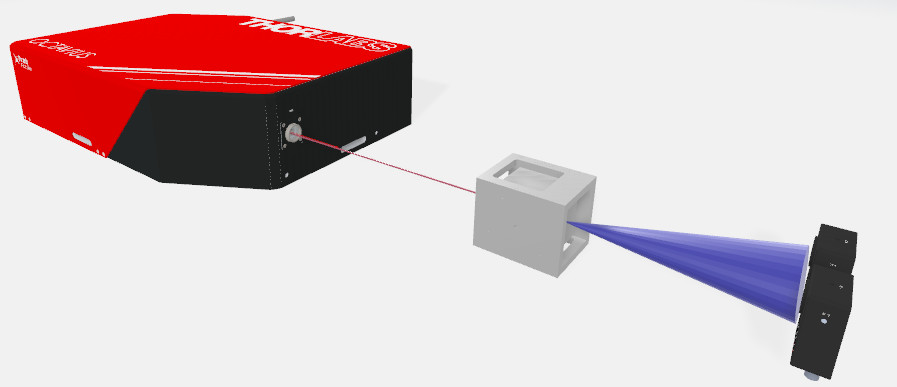
\includegraphics[width=\linewidth,height=2.8 cm]{images/TypeI.jpg}
\caption{SPDC type I}
\label{fig:type1}
\end{subfigure}
\begin{subfigure}[b]{0.45\linewidth}
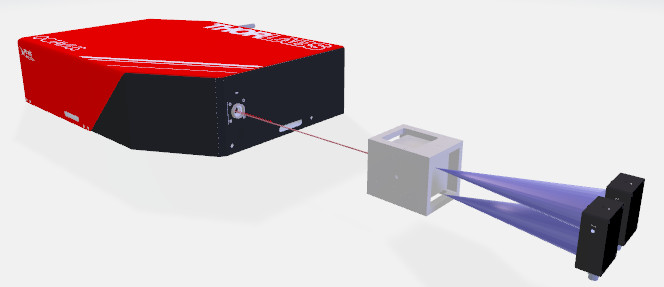
\includegraphics[width=\linewidth,height=2.8 cm]{images/typeII.jpg}
\caption{SPDC type II}
\label{fig:type2}
\end{subfigure}
\caption{An illustration of the SPDC type I (a) and II (b) processes, a laser incident on a non-linear crystal and photons coming out of it along cones.}
\label{fig:SPDC}
\end{figure}


Finally, in SPDC type-II the polarization of generated photons is orthogonal to each other. The photon with the polarization of the pump is called a signal photon. In this type of SPDC, each photon travels along its own cone. In this work, we are mainly concerned with the SPDC type-I process.

We will start our description of the SPDC process by considering the quantized electric field operator:

\begin{align}
\textbf{E}(\textbf{r},t)&=\textbf{E}^{(+)} (\textbf{r},t) + \textbf{E}^{(-)} (\textbf{r},t), \label{fiel+}
\end{align}

with

\begin{align}
\textbf{E}^{(+)} (\textbf{r},t)&=\frac{i(2 \pi \hbar w)^{\frac{1}{2}}}{\sqrt{V}} \sum_{\textbf{k},\nu}  \mathbf{a}_{\textbf{k},\nu} \mathbf{e}_{\textbf{k},\nu} e^{i(\textbf{k.r}-wt)}=[\textbf{E}^{(-)} (\textbf{r},t)]^{\dagger}, \label{quanfield}
\end{align}

where $w$ is the frequency of the electric field, $\mathbf{k}$ is the wave vector of all modes with defined linear momenta, we sum over this modes and polarizations as part of the canonical quantization process where we make a spatial Fourier expansion \cite{grynberg}, $\mathbf{e}_{\textbf{k},\nu}$ where $\nu=1,2$, is the polarization vector for a normal mode of wave vector $\mathbf{k}$ and defined polarization labeled by $\nu$, $\mathbf{a}_{\textbf{k},\nu}$ is the photon annihilation operator of the mode with wave vector $\mathbf{k}$ and polarization given by $\nu$. Finally, $V$ is the quantization volume, when we quantize we consider a finite volume (usually a cube) such that $k_{m}=\frac{2 \pi n_{m}}{L}$ where $m=x,y,z$ and $L$ is the length of said cube, the annihilation and creation operators must obey:

\begin{equation}
[\mathbf{a}_{\textbf{k},\nu},\mathbf{a^{\dagger}}_{\textbf{k},\nu}]=\delta_{\nu \nu'}\delta_{\textbf{k}\textbf{k'}},
\end{equation}

where $\delta_{ab}$ is the Kronecker's delta. The creation and annihilation operators act on the Fock basis as:

\begin{equation}
    \mathbf{a}_{\textbf{k},\nu}\ket{n}=\sqrt{n}\ket{n-1},\qquad
    \mathbf{a}_{\textbf{k},\nu}\ket{n}=\sqrt{n+1}\ket{n+1}.\label{Fock}
\end{equation}

The field operator $\textbf{E}^{(+)} (\textbf{r},t)$ acting on a vacuum $\ket{0}$, which means the absence of photons of wave vector $\mathbf{k}$ and polarization $\nu$, is given by:

\begin{equation}
\textbf{E}^{(+)} (\textbf{r},t)\ket{0}=0,
\end{equation}

 with the adjoint relation:

\begin{equation}
\bra{0}\textbf{E}^{(-)} (\textbf{r},t)=0.
\end{equation}

The Hamiltonian operator of a quantized electromagnetic field can be written as \cite{jackson}:

\begin{equation}
H=\frac{1}{2}\int_{V} d^{3}r (\mathbf{D \cdot E}+\mathbf{H \cdot B}),
\end{equation}

where $\textbf{D}$ and $\textbf{H}$ are the electric displacement and the magnetic field operators, respectively. These are given in terms of the electric field $\textbf{E}$ and the magnetic flux $\textbf{B}$ by means of the constitutive relations:


\begin{align}
\textbf{D}= \epsilon_{0} \textbf{E}+\textbf{P},\\
\textbf{H}=\frac{\textbf{B}}{\mu_{0}}-\textbf{M},
\end{align}

where $\epsilon_{0} $ is the permittivity and $\mu_{0}$ the permeability of free space, $\mathbf{P}$ is the electric polarization (the polarization) and $\mathbf{M}$ is the magnetic polarization (the magnetization) of the optical medium of interest (a non-linear crystal). In this work, we will neglect $\textbf{M}$ because we will assume that the laser beam is not intense enough to magnetize the crystal. Hence, the Hamiltonian becomes:

\begin{equation}
H=\frac{1}{2}\int_{V} d^{3}r \left(\epsilon_{0}\mathbf{E \cdot E}+\mathbf{E \cdot P}+\frac{\mathbf{B \cdot B}}{\mu_{0}} \right).
\end{equation}


As described in \cite{boyd}, while in linear optics polarization is often described by $\mathbf{P}(t)=\epsilon_{0} \chi^{(1)}\mathbf{E}(t)$, in nonlinear optics this equation is generalized by expressing the polarization as a power series of the field strenght:

\begin{equation}
\mathbf{P}(t)=\epsilon_{0} \left( \chi^{(1)}\mathbf{E}(t)+\chi^{(2)}\mathbf{E}^{2}(t)+\chi^{(3)}\mathbf{E}^{3}(t)+ \dots \right)=\mathbf{P}^{(1)}(t)+\mathbf{P}^{(2)}(t)+\mathbf{P}^{(3)}(t)+ \dots .
\end{equation}

 We will consider the polarization to have nonlinear components and the linear term to be included in a term we will call $H_{0}$
 
\begin{equation}
 H_{0}=\frac{1}{2}\int_{V} d^{3}r \left(\epsilon_{0}\mathbf{E \cdot E}+\mathbf{E} \cdot \mathbf{P^{(1)}}+\frac{\mathbf{B \cdot B}}{\mu_{0}} \right),
\end{equation}

  the zeroth order term or polar term is negligible because we are not considering polar media. The maincontribution to the SPDC is the second-order term in the nonlinear expansion which we will include in $H_{I}$:


\begin{equation}
H_{I}=\frac{1}{2} \int_{V} d^{3}r \textbf{E} \cdot \textbf{P}^{(2)}, \label{Hi}
\end{equation}

where

\begin{equation}
P_{i}^{(2)} (\mathbf{r},t)=\int_{0}^{\infty}dt_{1}\int_{0}^{\infty}dt_{2} \chi_{ijk}^{(2')}(t-t_{1},t-t_{2}) E_{j}(\textbf{r},t_{1}) E_{k}(\textbf{r},t_{2}), \label{polariza}
\end{equation}

and $\chi_{ijk}^{(2')}$ is related to the second-order nonlinear susceptibility and represents the response of the medium to the second power of the electric field. We will consider higher orders to be negligeable. By substituting Eq. \ref{polariza} in  Eq. \ref{Hi} and separating the field operators into its the creation and annihilation components, the interaction Hamiltonian $H_{I}$ turns into (we dropped the dependence of the fields to have a compact expression):

\begin{align*}
H_{I}=& \frac{1}{2} \int_{V}\int_{0}^{\infty}dt_{1}\int_{0}^{\infty}dt_{2} \chi_{ijk}^{(2')}(t-t_{1},t-t_{2}) \left( E_{i}^{(+)}E_{j}^{(+)}E_{k}^{(+)}+E_{i}^{(-)}E_{j}^{(+)}E_{k}^{(+)}\right.\\
&+ E_{i}^{(-)}E_{j}^{(-)}E_{k}^{(+)}+E_{i}^{(+)}E_{j}^{(-)}E_{k}^{(+)}+E_{i}^{(+)}E_{j}^{(+)}E_{k}^{(-)}+E_{i}^{(-)}E_{j}^{(+)}E_{k}^{(-)}\\
&+ \left.E_{i}^{(-)}E_{j}^{(-)}E_{k}^{(-)}+E_{i}^{(+)}E_{j}^{(-)}E_{k}^{(-)}  \right). \label{muchoscampos} \numberthis
\end{align*}

Since the SPDC process involves the annihilation of one photon of the pump beam and the creation of two photons of lower frequency, the only terms of Eq. \ref{muchoscampos} which are compatible with such phenomenon are those including $E_{i}^{(+)}E_{j}^{(-)}E_{k}^{(-)}$ (according to Eq. \ref{fiel+} the label $(+)$ is associated with the annihilation of photons and $(-)$ to their creation) and its Hermitian conjugate describing the reverse process. The other terms represent processes that do not preserve energy  so they will not be considered. Thus, the Hamiltonian $H_{I}$ reduces to:

\begin{equation}
H_{I}=\int_{V} d^{3}r \chi_{ijk}^{(2)}(w_{j},w_{k}) (E_{i}^{(+)}E_{j}^{(-)}E_{k}^{(-)})+\mathrm{H.c}, \label{Hi2}
\end{equation}

where  $\mathrm{H.c}$ means Hermitian conjugate and we redefined:


\begin{equation}
\chi_{ijk}^{(2)}(w_{j},w_{k})=\frac{1}{2}\int_{0}^{\infty}dt_{1}\int_{0}^{\infty}dt_{2} \chi^{(2')}_{ijk}(t-t_{1},t-t_{2}) e^{i w_{j} (t-t_{1})} e^{i w_{k} (t-t_{2})}.
\end{equation}

Substituting $t'=t-t_{1}$, $t''=t-t_{2}$ we may write:

\begin{equation}
\chi_{ijk}^{(2)}(w_{j},w_{k})=\frac{1}{2}\int_{0}^{\infty}dt'\int_{0}^{\infty}dt'' \chi^{(2')}_{ijk}(t',t'') e^{-i(w_{k}t'+w_{j}t'')}.
\end{equation}


Replacing the expressions for the fields in Eq. \ref{Hi2}, and now substituting $i, j, k$ for $s, i, p$, respectively, where $s, i, p$ refers to signal, idler and pump respectively, then approximating the sum to an integral (taking $V$ to $\infty$) we take $\sum_{\textbf{k}}\xrightarrow{}\frac{V}{(2\pi)^{3}}\int d^{3}k$ and $\delta_{ \mathbf{k} \mathbf{k}'} \xrightarrow{}\delta(\mathbf{k}-\mathbf{k}')$:

\begin{align*}
H_{I}= &\int d^{3}k_{p}\int d^{3}k_{s}\int d^{3}k_{i} \sum_{\nu_{p},\nu_{s},\nu_{i}}\chi_{ijk}^{(2)}(w_{p},w_{s},w_{i}) (\mathbf{e}_{k_{p},\nu_{p}})_{i} (\mathbf{e}_{k_{s},\nu_{s}})^{*}_{j} (\mathbf{e}_{k_{i},\nu_{i}})^{*}_{k} \\ & \times \mathbf{a}_{\nu_{p}}(\mathbf{k}_{p})\mathbf{a^{\dagger}}_{\nu_{s}}(\mathbf{k}_{s})\mathbf {a^{\dagger}}_{\nu_{i}}(\mathbf{k}_{i})e^{i(w_{s}+w_{i}-w_{p})t} \int_{V}d^{3}r e^{i \Delta\textbf{k} \cdot \textbf{r}}+\mathrm{H.c} , \label{jajaja} \numberthis
\end{align*}

where $\Delta \mathbf{k}= \mathbf{k}_{p}-\mathbf{k}_{s}-\mathbf{k}_{i}$ and:
\begin{align}
\chi_{ijk}^{(2)}(w_{p},w_{s},w_{i})=\frac{-iV^{\frac{3}{2}}}{(2\pi)^9 }(2 \pi \hbar)^{\frac{3}{2}} (w_{p}w_{s}w_{i})^{\frac{1}{2}}\chi_{ijk}^{(2)}(w_{s},w_{i}) .
\end{align}

As polarizations are fixed in SPDC, each sum in the labels $\nu_{p}, \nu_{s}, \nu_{i}$ contains only one term. Also, we will consider $\chi_{ijk}^{(2)}(w_{p},w_{s},w_{i})$ to vary so slowly (in $\mathbf{k}$ and $\mathbf{r}$) that we can treat it as a constant over the integrals. We will define $\chi= \chi_{ijk}^{(2)}(w_{p},w_{s},w_{i}) (\mathbf{e}_{k_{p},\nu_{p}})_{i} (\mathbf{e}_{k_{s},\nu_{s}})^{*}_{j} (\mathbf{e}_{k_{i},\nu_{i}})^{*}_{k}$ so we can write:

\begin{align*}
    H_{I}= &\chi \int d^{3}k_{p}\int d^{3}k_{s}\int d^{3}k_{i}\int_{V} d^{3}r \mathbf{a}_{\nu_{p}}(\mathbf{k}_{p})\mathbf{a^{\dagger}}_{\nu_{s}}(\mathbf{k}_{s})\mathbf {a^{\dagger}}_{\nu_{i}}(\mathbf{k}_{i})e^{i(w_{s}+w_{i}-w_{p})t} \\& e^{i \Delta\textbf{k} \cdot \textbf{r}}+\mathrm{H.c}. \numberthis{}
\end{align*}

$H_{0}$ is the electromagnetic field Hamiltonian, which is proportional to the number operator and only adds a global phase to our initial coherent state (the laser pump), which we can ignore \cite{leonhardt}. Our initial state is indeed a coherent state $\ket{\alpha_{p},0_{s},0_{i}}$ which turns into a coherent state plus two down converted photons $\ket{\alpha'_{p},1_{s},1_{i}}$.

In the interaction picture, the evolution of the state of the system is given by the equation:


\begin{align}
i \hbar \frac{d}{dt}\ket{\psi(t)}&=H_{I}\ket{\psi(t)}.\label{a}
\end{align}

Since this is a first order differential equation in time, the state of the system $\ket{\psi(t)}$ is completely determined by the initial condition, say $\ket{\psi(t_{0})}$, then we may write:

\begin{equation}
    \ket{\psi(t)}=U(t,t_{0})\ket{\psi(t_{0})},
\label{b}
\end{equation}

where $U(t,t_{0})$ is the evolution operator and it encodes the dynamics of the system in the interval $[t_{0},t]$. Substituting Eq. \ref{b} in Eq. \ref{a} one arrives to: 

\begin{align}
i \hbar \frac{d}{dt}U(t,t_{0})=H_{I}U(t,t_{0}).
\end{align}

The solution to this initial value problem can be expressed  as an iterative integral equation by direct integration, commonly known as Dyson series \cite{zettili}, Moreover according to \ref{b}, the evolution operator $U(t,t_{o})$ must also satisfy the initial condition $U(t_{0},t_{0})=\mathbf{1}$, thus up to first order in $H_{I}$, we have:

\begin{equation}
U(t,to)=\mathbf{1}-\frac{i}{\hbar} \int_{t_{0}}^{t} H_{I} (\tau) d\tau=\mathbf{1}+U_{1}.
\end{equation}

We will not consider higher orders for two reasons: we are interested in the SPDC process as a single-photon states source (second-order in the evolution operator would generate four photons), and higher orders are unlikely because the laser pump is not as intense as for four photons to be produced in the crystal at once.

Now, to analyze the evolution of the system in the SPDC process we need to identify the initial state. Knowing that initially, we have a pump laser beam and no photons in the signal or idler channels, we can identify the initial state as composed by a coherent state in the input channel and vacuum states of the quantized electromagnetic field in the output channels. A coherent state is a superposition of Fock states in the following form \cite{leonhardt}:

\begin{equation}
\ket{\alpha}=e^{\frac{-|\alpha|^{2}}{2}} \sum_{n=0}^{\infty} \frac{\alpha^{n}}{\sqrt{n!}} \ket{n},
\end{equation}

where $\alpha$ is a complex parameter known as the complex wave amplitude. Coherent states are eigenstates of the annihilation operator with eigenvalue $\alpha$

\begin{equation}
\hat{\mathbf{a}}\ket{\alpha}=\alpha\ket{\alpha},
\end{equation}

fullfiling the following properties:

\begin{align}
\langle H \rangle = \hbar w_{p} \left(|\alpha|^{2}+\frac{1}{2}\right),\qquad P_{n}=e^{-\langle n\rangle}\frac{\langle n \rangle^{n}}{n!},
\end{align}

where $P_{n}$ is the probability of finding $n$ photons in a measurement of the coherent state. This probability corresponds to a Poisson distribution so that the coherent state obeys Poissonian statistics.

Thus our initial state can be cast in the form $\ket{\psi(t_{0})}=\ket{\alpha_{p},0_{s},0_{i}}$, where the labels $p, s, i$ stand for the pump, signal and idler channels. Let us analyze the action of the second order term of the Dyson series  $U_{1}$ on the initial state:

\begin{align*}
 U_{1}\ket{\psi(t_{0})}= &\frac{-i \chi}{\hbar}  \int_{t_{0}}^{t} d\tau \int d^{3}k_{p}\int d^{3}k_{s}\int d^{3}k_{i}\int_{V} d^{3}r \alpha_{p} (\mathbf{k}_{p},w_{p})\\ &e^{i(w_{s}+w_{i}-w_{p})\tau}e^{i \Delta\textbf{k}.\textbf{r}}\ket{\alpha_{p},1_{s},1_{i}} , \numberthis{}\label{t1}
\end{align*}


In the last expressions, we used Eqs. \ref{Fock}  concerning the action of the ladder operators on the initial state. Note that the initial state is annihilated by the action of the term $\mathrm{H.c}$ in Eq. \ref{jajaja}.  If we define 

\begin{equation}
 \xi(t,t_{0})=\frac{-i\chi}{\hbar}  \int d^{3}k_{p}\int d^{3}k_{i} \int d^{3}k_{s}    \int_{t_{0}}^{t} d\tau e^{i(w_{s}+w_{i}-w_{p})\tau}  
\int_{V} d^{3}r  e^{i \Delta\textbf{k} \cdot\textbf{r}} ,
\end{equation}



we can then rewrite Eq. \ref{t1} as:

\begin{equation}
U_{1}(t,t_{0})\ket{\alpha_{p},0_{s},0_{i}}=\xi(t,t_{0}) \mathbf{a_{p}}\mathbf{a_{s}^{\dagger}}\mathbf{a_{i}^{\dagger}}\ket{\alpha_{p},0_{s},0_{i}}=\xi(t,t_{0}) \alpha_{p} \ket{\alpha_{p},1_{s},1_{i}}.
\end{equation}

Finally, we may write

\begin{equation}
    U(t,t_{0})\ket{\alpha_{p},0_{s},0_{i}}=(\mathbf{1}+\xi(t,t_{0}) \mathbf{a_{p}}\mathbf{a_{s}^{\dagger}}\mathbf{a_{i}^{\dagger}})\ket{\alpha_{p},0_{s},0_{i}}. \label{evo}
\end{equation}

This equation represents the superposition of our initial coherent state on the pump channel, and the same coherent state with two down-converted photons, one in the idler channel and the other one in the signal channel, thus describing the SPDC process as intended. In this section, we developed the basics of the quantum theory of the SPDC process. In the next section, we will use this theory to explore spatial correlations between the idler a signal photons.

\subsection{First order joint amplitude function}

Now that we have presented a quantum mechanical description of the phenomenon, we will describe how it can be used to generate single-photon states. We will use the model proposed by O. Rosas-Ortiz and L.M Procopio in \cite{procopio} in order to set the design for our experiment. Most information concerning the spatial correlations, if not all, is encoded in the joint amplitude function, which is the aim of the present section. 



  Our final state can be calculated using the first order evolution operator given by \ref{evo}:

\begin{align*}
\ket{\psi(t)}=& U(t)\ket{\psi(t_{0})},\numberthis{}\\
=& \ket{\alpha_{p},0_{s},0_{i}}-\frac{i \chi}{\hbar}  \int_{t_{0}}^{t} d\tau \int d^{3}k_{p}\int d^{3}k_{s}\int d^{3}k_{i}\int_{V} d^{3}r \alpha_{p} (\mathbf{k}_{p},w_{p})\\ &\times e^{i(w_{s}+w_{i}-w_{p})\tau}e^{i \Delta\textbf{k}.\textbf{r}}\ket{\alpha_{p},1_{s},1_{i}}  \numberthis{}
\end{align*}

We will rewrite this as:

\begin{equation}
\ket{\psi(t)}=\ket{\alpha_{p},0_{s},0_{i}}-\frac{i\chi}{\hbar} \int d^{3}k_{s}\int d^{3}k_{i}
\Phi(\mathbf{k}_{i},w_{i},\mathbf{k}_{s},w_{s})\ket{\alpha_{p},1_{s},1_{i}},
\end{equation}

where we conveniently defined $\Phi$:

\begin{equation}
\Phi(\mathbf{k}_{i},w_{i},\mathbf{k}_{s},w_{s})=\int d^{3}k_{p} \alpha_{p}(\mathbf{k}_{p},w_{p}) \int_{V} d^{3}r e^{i \Delta \mathbf{k}.\mathbf{r}} \int_{t_{0}}^{t} d\tau e^{i(w_{s}+w_{i}-w_{p})\tau}.\label{jointd}
\end{equation}

This $\Phi$ function is known as the first order joint amplitude function, it is of first-order because we stopped the Dyson series at first order. This function will enable us to study spatial correlations of the signal and idler channel in the next section.

\subsection{Spatial correlations}

Let us now study the spatial correlations from the joint amplitude function, to do this a couple of approximations will be made.
Considering steady state fields and that the dimensions of the nonlinear crystal are much larger than the wavelength of the pump, meaning we consider $V\xrightarrow{}\infty$, we can approximate the following integrals:


\begin{align*}
&\int_{t_{0}}^{t} d\tau e^{i(w_{s}+w_{i}-w_{p})\tau} \xrightarrow{}
\int_{-\infty}^{\infty} d\tau e^{i(w_{s}+w_{i}-w_{p})\tau}= 2\pi \delta(w_{s}+w_{i}-w_{p}) ,\\
&\int_{V} d^{3}r  e^{i \Delta\textbf{k} \cdot\textbf{r}} \xrightarrow{} \int_{-\infty}^{\infty} d^{3}r  e^{i \Delta\textbf{k} \cdot \textbf{r}}=(2 \pi)^{3}  \delta(\mathbf{k}_{p}-\mathbf{k}_{s}-\mathbf{k}_{i}) .
\label{t2} \numberthis{}
\end{align*}

Implementing such approximations the Eq. \ref{jointd} becomes:

\begin{equation}
\Phi(\mathbf{k}_{i},w_{i},\mathbf{k}_{s},w_{s})= \eta \alpha_{p}(\mathbf{k}_{s}+\mathbf{k}_{i},w_{s}+w_{i}) ,
\end{equation}


where $\eta$ is a global factor. Let us assume  $\alpha_{p}$ can be factorized into two functions, one depending on the wave vectors, and one depending on the frequencies:

\begin{equation}
\Phi(\mathbf{k_{i}},w_{i},\mathbf{k_{s}},w_{s})= \eta G(\mathbf{k}_{i}+\mathbf{k}_{s}) F(w_{s}+w_{i}) .
\end{equation}
 
We  will now separate the wave vectors into their transversal and longitudinal components:

\begin{equation}
\mathbf{k}_{r}=\mathbf{q}_{r}+k_{rz} \mathbf{e}_{rz},\qquad \mathbf{q}_{r}=q_{rx} \mathbf{e}_{rx}+q_{ry} \mathbf{e}_{ry},
\end{equation}

where $r=p, s, i$. We will assume the paraxial approximation to be valid,  as Molina-Terriza and Minardi \cite{minardi} demonstrated that in this situation the transversal components are negligeable with respect to the longitudinal one. Moreover, we are assumming that both functions $G$ and $F$ are Gaussian so that:

\begin{equation}
G(\mathbf{A})=e^{- (\sigma \abs{\mathbf{A}})^{2} },\qquad F(w)=e^{-(\delta w)^2},
\end{equation}

we can rewrite the joint amplitude function as:

\begin{equation}
\Phi(\mathbf{q}_{i},w_{i},\mathbf{q}_{s},w_{s})= \eta e^{-\sigma^{2}\abs{\mathbf{q_{s}}+\mathbf{q_{i}}}^{2}} F(w_{s}+w_{i}).\label{true}
\end{equation}

The spatial and spectral sensitivity of the detector are assumed to be given by Gaussian profile filters:

\begin{equation}
\mathbb{F}_{s}(\mathbf{q}_{r})=e^{-\abs{\mathbf{\sigma}.\mathbf{q}_{r}}^{2}},\qquad \mathbb{F}_{f}(w_{r})=e^{-(\alpha_{r} w_{r})^{2}}. \label{filter}
\end{equation}

\begin{figure}[t!]


\centering
\begin{subfigure}[b]{0.45\linewidth}
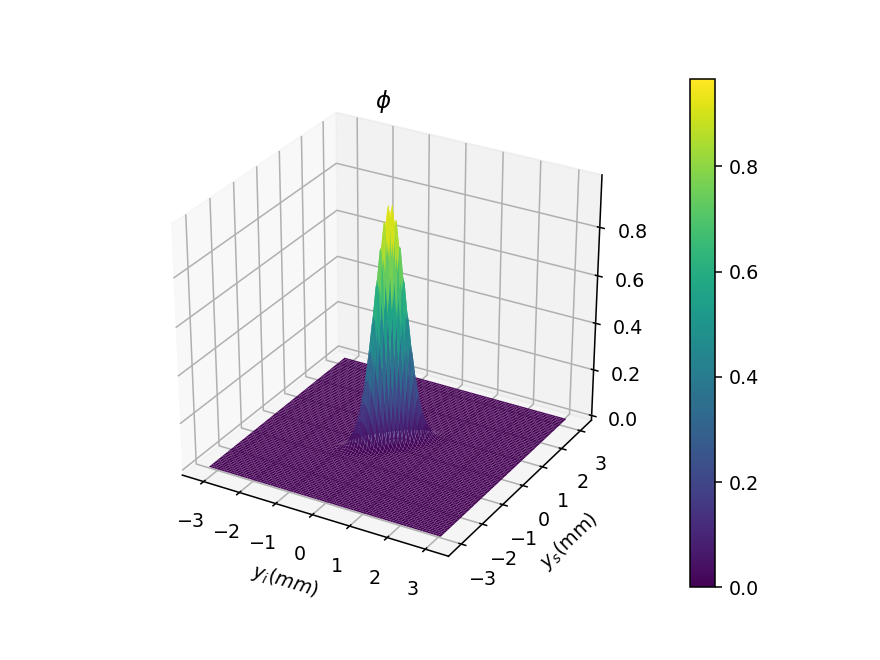
\includegraphics[width=\linewidth]{images/SPDC_yy.png}
\caption{YY correlation}
\end{subfigure}
\begin{subfigure}[b]{0.45\linewidth}
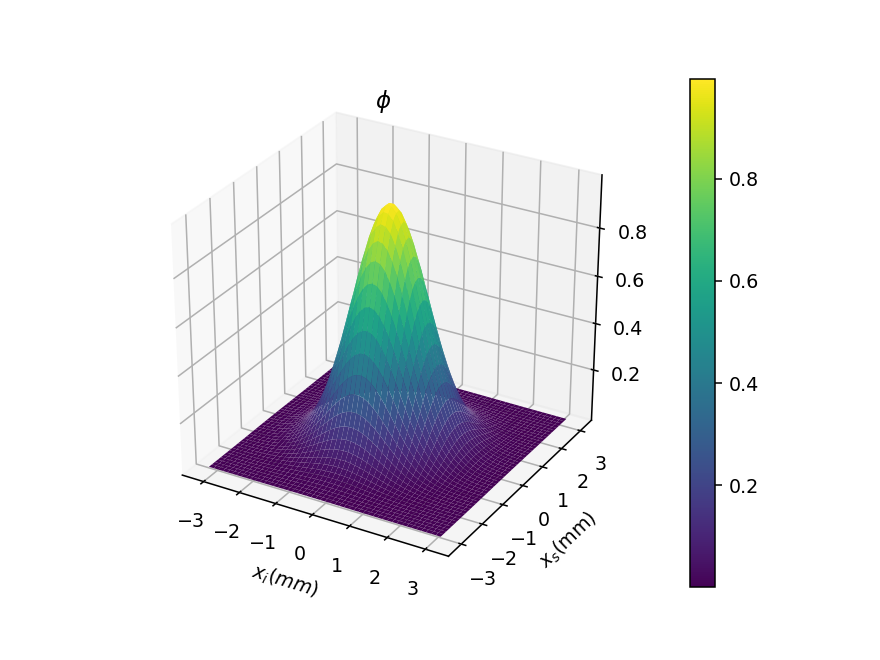
\includegraphics[width=\linewidth]{images/SPDC_xx.png}
\caption{XX correlation}
\end{subfigure}
\begin{subfigure}[b]{0.45\linewidth}
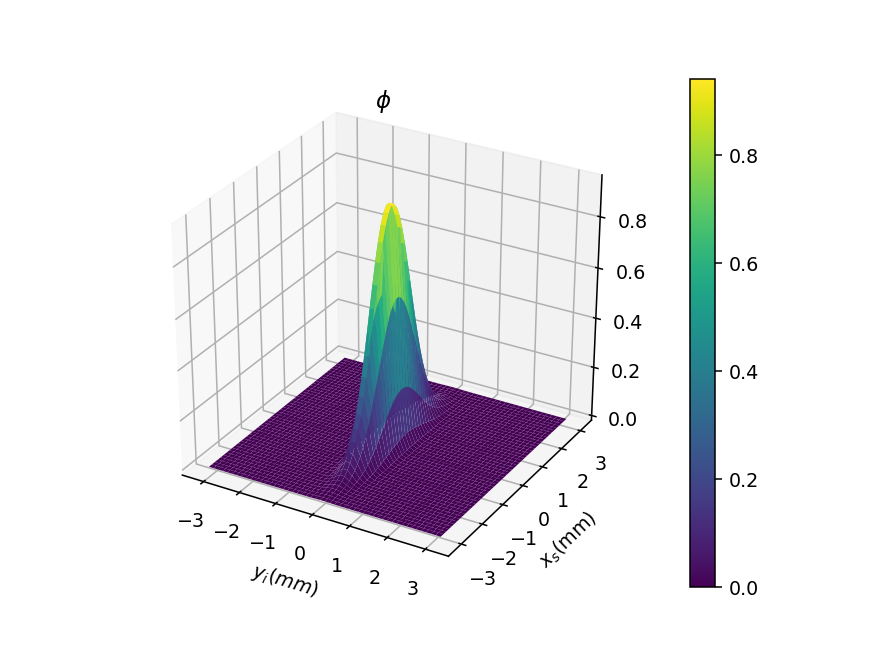
\includegraphics[width=\linewidth]{images/SPDC_yx.png}
\caption{YX correlation}
\end{subfigure}
\begin{subfigure}[b]{0.45\linewidth}
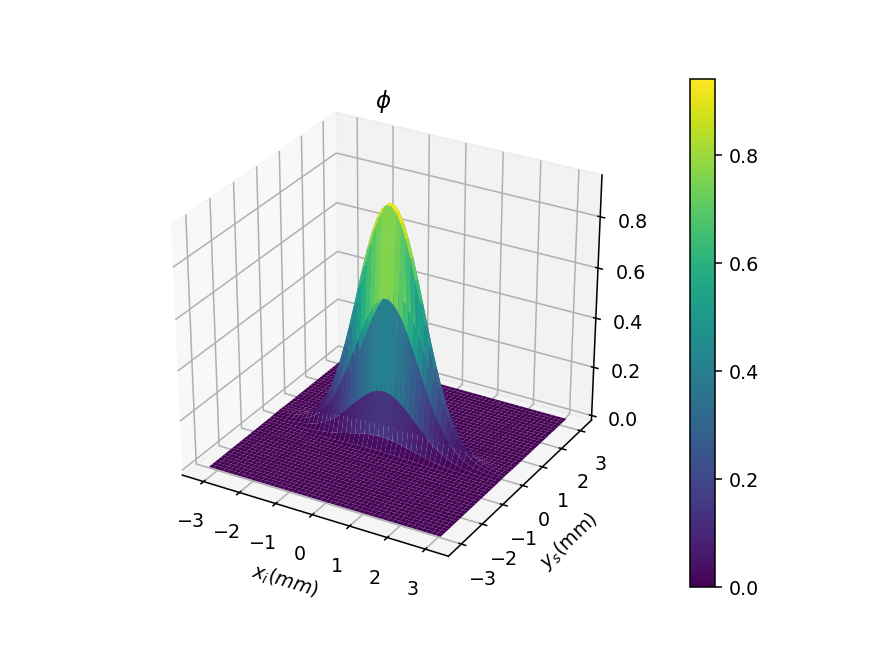
\includegraphics[width=\linewidth]{images/SPDC_xy.png}
\caption{XY correlation}
\end{subfigure}
\caption{Plots for $\Phi_{s}(x_{i},y_{i},x_{s},y_{s})$  from left to right are $x_{s}=x_{i}=0$ (a), $y_{s}=y_{i}=0$ (b), $x_{i}=y_{s}=0$ (c) and $y_{i}=x_{s}=0$ (d). In all these plots we set $\sigma=0.18$, $\sigma_{x}=0.59$, $\sigma_{y}=0.1$.}
\label{SPDC}
\end{figure}

Here $\mathbf{\sigma}=(\sigma_{rx},\sigma_{ry})$, and $\alpha_{r}$, correspond to the spatial and frequency collection modes respectively, the physical process is modeled by Eq. \ref{true}, however, our detectors and filters are only efficient up to a certain point, in order to account for it we multiply the response of the filter Eq. \ref{filter} to our process so we can write:
 
\begin{equation}
\Phi(\mathbf{q}_{i},w_{i},\mathbf{q}_{s},w_{s})=\Phi_{f}(w_{i},w_{s})\Phi_{s}(\mathbf{q}_{i},\mathbf{q}_{s}).
\end{equation}

where we grouped the functions depending merely on frequencies $w$  and the functions depending on the variables $\mathbf{q}$ as

\begin{equation}
\Phi_{f}(w_{s},w_{i})= \eta F_{p}(w_{s}+w_{i}) \mathbb{F}_{f}(w_{i})\mathbb{F}_{f}(w_{s})
\end{equation}

\begin{equation}
 \Phi_{s}(\mathbf{q}_{i},\mathbf{q}_{s})=e^{-\sigma^{2}\abs{\mathbf{q}_{s}+\mathbf{q}_{i}}^{2}}\mathbb{F}_{s}(\mathbf{q}_{s})\mathbb{F}_{s}(\mathbf{q}_{i}).
\end{equation}

Since we are in momentum space, we can obtain the spatial correlations by taking the Fourier transform:

\begin{equation}
\Phi_{s}(\mathbf{x}_{i},\mathbf{x}_{s})=\mathscr{F}(\Phi_{s}(\mathbf{q}_{i},\mathbf{q}_{s}))=N \int d^{2}q_{i} \int d^{2}q_{s} \Phi_{q}(\mathbf{q}_{i},\mathbf{q}_{s}) e^{-i \mathbf{q}_{s}.\mathbf{r}_{s}} e^{-i \mathbf{q}_{i}.\mathbf{r}_{i}}.
\end{equation}




This last equation encodes the spatial correlations between the signal and idler photon channels, allowing us to use this scheme to study single-photon states, by measuring in two positions which are highly correlated which we can see from Fig. \ref{SPDC} is a region of just a few millimeters, and only taking into account measurements where both detectors (one placed in the signal channel and the other in the idler channel) click, ensuring that this process took place and we indeed have single-photon states.


\section{The lossless beam splitter}


In this chapter, we will develop the classical and quantum theory of the most important optical element in this thesis, the beam splitter. The beam splitter is a four-port optical device with two inputs and two outputs, as shown in Fig. \ref{fig:BS}, in which two input beams may interfere to produce two outgoing beams. A beam splitter usually consists of two dielectric triangular prisms spliced in the form of a cube.

\subsection{The  classical lossless beam splitter}

This section is inspired in the beam splitter description presented in \cite{ludon} and \cite{leonhardt}. We will consider monochromatic light and we will assume that the beam splitter is an ideal reversible and lossless device.


In describing the behaviour of a laser beam in classical electrodynamics, it is common to consider the study of their corresponded electric fields, if the beams cross through a linear medium, the outgoing fields can be written as linear combinations of the input fields satisfying the proper boundary conditions \cite{jackson}. In the beam splitter we have two inputs and two outputs, the output fields $E_{1}'$ and $E_{2}'$  can be written in terms of the input fields $E_{1}'$ and $E_{2}'$ as:

\begin{equation}
\begin{pmatrix} E_{1}' \\ E_{2}' \end{pmatrix}=B\begin{pmatrix} E_{1} \\ E_{2} \end{pmatrix},\label{rule}
\end{equation}

the linear transformation $B$ represents the action of the beam splitter on the input fields and is described by a matrix:

\begin{equation}
B=\begin{pmatrix} B_{11}& B_{12} \\B_{21} & B_{22} \end{pmatrix}.
\end{equation}

\begin{figure}[t!]
\centering
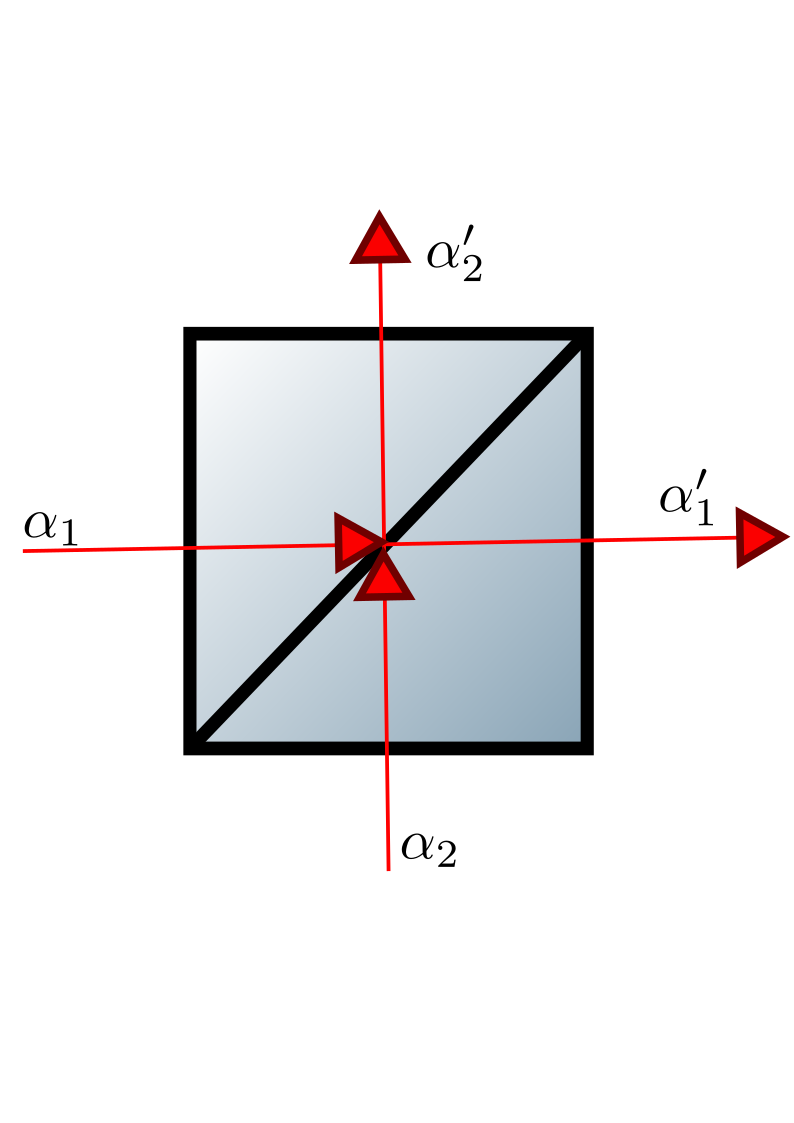
\includegraphics[width=5 cm,height=5 cm]{images/bS.png}
\caption{A Beam splitter cube.}
\label{fig:BS}
\end{figure}

The conditions  that must be fulfilled by the matrix elements $B_{ij}$  $i,j=1,2$  can be established by demanding the total intensity to be preserved (recall that we are considering that the beam splitter is a lossless device), that is:

\begin{align*}
I_{1}'+I_{2}'=&I_{1}+I_{2},\numberthis \\
I_{1}'\propto&|B_{11} E_{1}|^{2}+|B_{12} E_{2}|^{2}+B_{11} B_{12}^{*} E_{1} E_{2}^{*}+B_{11}^{*} B_{12} E_{1}^{*} E_{2},\numberthis \\
I_{2}'\propto&|B_{21} E_{1}|^{2}+|B_{22} E_{2}|^{2}+B_{21} B_{22}^{*} E_{1} E_{2}^{*}+B_{21}^{*} B_{22} E_{1}^{*} E_{2},\numberthis\\
|E_{1}|^{2}+|E_{2}|^{2}=&(|B_{21}|^{2}+|B_{11}|^{2})|E_{1}|^{2}+(|B_{12}|^{2}+|B_{22}|^{2})|E_{2}|^{2}\\
&+(B_{21} B_{22}^{*}+B_{11} B_{12}^{*})E_{1} E_{2}^{*}+(B_{21}^{*} B_{22}+B_{11}^{*} B_{12})E_{1}^{*} E_{2}, \numberthis
\end{align*}

where $I_{1}$ and $I_{2}$ are the intensities of the input fields and $I_{1}'$ and $I_{2}'$ are the intensities of the output fields. Recall that the intensity of a given electric field is given by $I=\frac{c n \epsilon_{0}}{2} |E|^{2}$, where $c$ is the speed of light, $n$ the index of refraction of the medium and $\epsilon_{0}$ is the permitivity of free space. The conservation of intensity (energy) leads us to the following relationships:

\begin{equation}
|B_{12}|^{2}+|B_{22}|^{2}=|B_{21}|^{2}+|B_{11}|^{2}=1,\qquad B_{21}^{*} B_{22}+B_{11}^{*} B_{12}=0.
\end{equation}

These relations imply that the matrix $B$ is unitary. Yet, from this set of equations, one can derive another constraint on the coefficients, namely, $B_{21}^{*} B_{11}+B_{22}^{*} B_{12}=0$. This is consistent with the fact that $B^{\dagger}B=B^{\dagger}B= \mathbf{1}$. For our purposes, it will be convenient to write the matrix $B$ in terms of the reflection coefficient $\rho$ and the transmission coefficient $\tau$, the transmission coefficient is a measure of how much light is transmitted through a material in relation to the amount of light incident on it, the reflection coefficient is a similar measure for reflection on the material. These coefficients fulfill the relationship:

\begin{equation}
|\tau|^{2}+|\rho|^{2}=1.
\end{equation}
 
 In the classical regime the transformation $B$ is usually written as:
 
 \begin{equation}
 B=\begin{pmatrix} \tau & \rho \\ -\rho & \tau \end{pmatrix},
 \end{equation}


so then the transformation rule \ref{rule} reads

\begin{equation}
\begin{pmatrix} E_{1}' \\ E_{2}' \end{pmatrix}=\begin{pmatrix} \tau & \rho \\ -\rho & \tau \end{pmatrix} \begin{pmatrix} E_{1} \\ E_{2} \end{pmatrix}.
\end{equation}




\subsection{The quantum lossless beam splitter}

Now, we will describe the quantum theory of a lossless beam splitter. To do this we will first consider the quantized electric field and then we will establish the theory. 


The electric field of a polarized and monochromatic light beam can be written as:

\begin{equation}
\mathbf{E}=i \mathbf{\epsilon}N w \left( \alpha e^{i (\mathbf{k \cdot r}-w t)}+\alpha^{*} e^{-i (\mathbf{k \cdot r}-w t)} \right),
\end{equation}

where $\alpha$ is known as the complex wave amplitude. To obtain a theoretical model of a beam splitter as general as possible, let us describe the device as a four-port device, a black box with two input and two output ports.

If two coherent light beams with complex wave amplitudes $\alpha_{1}$ and $\alpha_{2}$ enter the beam splitter we expect the output complex wave amplitudes  are superimposed according to a linear transformation that we will call also $B$ as

\begin{equation}
\begin{pmatrix} \alpha_{1}' \\ \alpha_{2}' \end{pmatrix}=B\begin{pmatrix} \alpha_{1} \\ \alpha_{2} \end{pmatrix}. \label{ladilla}
\end{equation}

When the electric field  is quantized, the complex wave amplitude $\alpha$ is promoted to an annihilation operator \cite{ludon}. Once quantized the relation \ref{ladilla} becomes:

\begin{equation}
\begin{pmatrix} \mathbf{a}_{1}' \\ \mathbf{a}_{2}' \end{pmatrix}=B\begin{pmatrix} \mathbf{a}_{1} \\ \mathbf{a}_{2} \end{pmatrix}.
\label{eq:amplitudes}
\end{equation}

This equation describes the transformation of the ladder operators in the process, in the Heisenberg picture. Assuming the incoming and outgoing beams are both independent bosonic modes, we obtain some properties of the $B$ matrix as a consequence of the ladder operators commutation relationships:

\begin{align}
&[\mathbf{a}'_{\nu},\mathbf{a}'_{\mu}]=[\mathbf{a}_{\nu},\mathbf{a}_{\mu}]=0,\\
&[\mathbf{a}'_{\nu},\mathbf{a}'^{\dagger}_{\mu}]=[\mathbf{a}_{\nu},\mathbf{a}^{\dagger}_{\mu}]=\delta_{\mu \nu},
\label{commutators}
\end{align}

where $\mu=1,2$ and $\nu=1,2$. From Eq. \ref{eq:amplitudes} it follows that:

\begin{align}
&\mathbf{a}'_{\mu}=B_{\mu 1}\mathbf{a}_{1}+B_{\mu 2} \mathbf{a}_{2}, \\
&\mathbf{a}'^{\dagger}_{\mu}=B_{\mu 1}^{*}\mathbf{a}^{\dagger}_{1}+B_{\mu 2}^{*} \mathbf{a}^{\dagger}_{2}.
\label{combined amplitudes}
\end{align}

Then using Eq. \ref{combined amplitudes} and Eq. \ref{commutators} we find 

\begin{equation}
   [\mathbf{a}'_{\nu},\mathbf{a}'^{\dagger}_{\mu}]=B_{\nu 1} B_{\mu 1}^{*}+B_{\nu 2} B_{\mu 2}^{*} .
\end{equation}

Substituting all the possible values of $\nu$ and $\mu$ we find the following relationships:

\begin{equation}
|B_{11}|^{2}+|B_{12}|^{2}=|B_{21}|^{2}+|B_{22}|^{2}=1 ,\qquad B_{11} B_{21}^{*}+B_{12} B_{22}^{*}=0.
\end{equation}

As in the classical case, we find the $B$ transformation to be unitary, something expected as the beam splitter is still a lossless device. The most general form of a unitary $2\times2$ matrix is \cite{leonhardt}:


\begin{equation}
B=e^{i\Lambda} \begin{pmatrix} e^{i\frac{\phi}{2}} & 0 \\ 0 & e^{-i\frac{\phi}{2}} \end{pmatrix} \begin{pmatrix} \cos(\theta) &  \sin(\theta) \\ - \sin(\theta) & \cos(\theta) \end{pmatrix} \begin{pmatrix} e^{i\frac{\psi}{2}} & 0 \\ 0 & e^{-i\frac{\psi}{2}} \end{pmatrix} \label{unitary},
\end{equation}

where $\psi$, $\Lambda$, $\theta$, $\phi$ are real parameters in the interval $[0,2\pi)$. So far our analysis is valid for any linear and lossless four-port device. Furthermore, from Eq. \ref{unitary} we can see that any four-port device can be considered as acting in three steps. First, the phases of the incident modes are changed\footnote{A phase shifter is denoted by $P_{\phi}=e^{i \frac{\phi}{2}}\begin{pmatrix}e^{i \frac{\phi}{2}} & 0 \\0 & e^{-i \frac{\phi}{2}} \end{pmatrix}$}, then the amplitudes are mixed (rotated) and then the phases are changed again. In most cases, we can adjust the reference phases such that only the rotation is important (a reference phase is the phase from which we start measuring phase-shifts). From now on we will parametrize our beam splitter ($BS$) as:

\begin{equation}
BS=\begin{pmatrix} \cos(\theta) & i \sin(\theta) \\ i \sin(\theta) & \cos(\theta) \end{pmatrix},\label{BS_matrix}
\end{equation}


this corresponds to  setting $\Lambda=0$, $\phi=-\psi=\frac{\pi}{2}$. The difference between $B$ and $BS$ is that $B$ is a general unitary matrix and in $BS$ we fixed the parameters that involve phase-shifting and the global phase. Let us now analyze this optical element in the Fock basis  to use it on a single-photon state. In the Heisenberg picture operators evolve via the evolution operator:

\begin{equation}
\begin{pmatrix} \mathbf{a}'_{1} \\ \mathbf{a}'_{2}\end{pmatrix}=\mathbf{U}^{\dagger}_{B} \begin{pmatrix} \mathbf{a}_{1} \\ \mathbf{a}_{2}\end{pmatrix} \mathbf{U}_{B}.
\label{Heisenberg}
\end{equation}

A Fock state $\ket{n_{1},n_{2}}$ ($\ket{n_{1},n_{2}}'$), meaning $n_{1}$ photons in the first input (output) and $n_{2}$ photons in the second input (output), can be generated from a vacuum state through the subsequent application on creation operators  $\mathbf{a}^{\dagger}_{1}\mathbf{a}^{\dagger}_{2}$. 

\begin{equation}
 \ket{n_{1},n_{2}}=\frac{1}{\sqrt{n_{1}! n_{2}!}} (\mathbf{a}_{1}^{\dagger})^{n_{1}}(\mathbf{a}_{2}^{\dagger})^{n_{2}} \ket{0,0}.
\end{equation}

Note that if just one of the input channels is pumped, then the state corresponding to the other one is a vacuum state $\ket{0}$. Correspondingly, in the Schrodinger picture a state $\ket{\psi}$ evolves by means of the rule:

\begin{equation}
 \ket{\psi}'=U_{B}\ket{\psi},
\end{equation}

so for the vacuum state we have:
\begin{equation}
 \ket{0,0}'=U_{B}\ket{0,0}.
 \label{evolution}
\end{equation}

The evolution of a Fock state $\ket{n_{1},n_{2}}'$:

\begin{align}
&\ket{n_{1},n_{2}}'=U_{B}\ket{n_{1},n_{2}},\\
&\ket{n_{1},n_{2}}'=\frac{U_{B}}{\sqrt{n_{1}! n_{2}!}} (\mathbf{a}_{1}'^{\dagger})^{n_{1}}(\mathbf{a}_{2}'^{\dagger})^{n_{2}} \ket{0,0}.
\end{align}

From Eq. \ref{Heisenberg}, Eq. \ref{eq:amplitudes} and Eq. \ref{evolution} we can obtain:

\begin{align}
&\ket{n_{1},n_{2}}' =\frac{U_{B}}{\sqrt{n_{1}! n_{2}!}} (\mathbf{a}_{1}'^{\dagger})^{n_{1}}(\mathbf{a}_{2}'^{\dagger})^{n_{2}} U^{\dagger}_{B}\ket{0,0}',\\
&\ket{n_{1},n_{2}}' =\frac{1}{\sqrt{n_{1}! n_{2}!}} (\mathbf{a}_{1}^{\dagger})^{n_{1}}(\mathbf{a}_{2}^{\dagger})^{n_{2}}\ket{0,0}'.
\end{align}

By writing the original ladder operators in terms of the transformed ladder operators given by Eq. \ref{eq:amplitudes}, and applying Newton's binomial formula (we can do this because the operators commute, in general this cannot be done) we arrive at the expression \footnote{ The binomial coefficient is $\begin{pmatrix} n \\ k \end{pmatrix} =\frac{n!}{\sqrt{k!(n-k)!}}$}:

\begin{align*}
\ket{n_{1},n_{2}}' = &\frac{1}{\sqrt{n_{1}! n_{2}!}} (B_{11}\mathbf{a}_{1}'^{\dagger}+B_{21}\mathbf{a}_{2}'^{\dagger})^{n_{1}}(B_{12}\mathbf{a}_{1}'^{\dagger}+B_{22}\mathbf{a}_{2}'^{\dagger})^{n_{2}}\ket{0,0}',\\
\ket{n_{1},n_{2}}'= &\frac{1}{\sqrt{n_{1}! n_{2}!}}\sum^{n_{1},n_{2}}_{k_{1},k_{2}=0}\begin{pmatrix} n_{1} \\ k_{1} \end{pmatrix}\begin{pmatrix} n_{2} \\ k_{2} \end{pmatrix} B_{11}^{n_{1}-k_{1}} B_{21}^{k_{1}} B_{12}^{n_{2}-k_{2}} B_{22}^{k_{2}} \\
&\times \sqrt{(n_{1}+n_{2}-k_{1}-k_{2})!(k_{1}+k_{2})!} \ket{n_{1}+n_{2}-k_{1}-k_{2},k_{1}+k_{2}}' .\numberthis{}
\end{align*}

Let us consider the particular example  $n_{1}=n$ and $n_{2}=0$  and vice-versa (from now on we will drop the primes on the right hand side):
\begin{equation}
 \ket{n,0}'=\sum^{n}_{k=0} \sqrt{\frac{n!}{(n-k)!k!}} B_{11}^{n-k} B_{21}^{k} \ket{n-k,k}
\end{equation}
and its counterpart
\begin{equation}
     \ket{0,n}'=\sum^{n}_{k=0} \sqrt{\frac{n!}{(n-k)!k!}} B_{12}^{n-k} B_{22}^{k} \ket{n-k,k}.
\end{equation}

In this work will consider single-photon states in the input channels, so that our case of interest is $n=1$,we expand the sum to obtain:

\begin{align}
\ket{1,0}'=B_{11}\ket{1,0}+B_{21}\ket{0,1},\label{basis2} \\
\ket{0,1}'=B_{12}\ket{1,0}+B_{22}\ket{0,1}.
\label{basis}
\end{align}


From Eqs. \ref{basis2}-\ref{basis}, we can see that the evolution of a single-photon state can be written in terms of the $BS$ matrix if we define an appropriate basis to describe the system. We will use the Horizontal-Vertical computational basis:

 \begin{equation}
 \ket{1}=\ket{1}_{h}\ket{0}_{v}=\begin{pmatrix} 1 \\0\end{pmatrix},
 \end{equation}

 means one photon in the horizontal path and vacuum in the vertical one, and
 
 \begin{equation}
 \ket{2}=\ket{0}_{h}\ket{1}_{v}=\begin{pmatrix} 0 \\1 \end{pmatrix},
 \end{equation}
 
means vacuum  in the horizontal path and one photon in the vertical one. In this basis Eq. \ref{basis} becomes:

\begin{equation}
\ket{out}=\begin{pmatrix} \cos(\theta) & i \sin(\theta) \\ i \sin(\theta) & \cos(\theta) \end{pmatrix} \ket{in},
\end{equation}

where $\ket{in}=\ket{1},\ket{2}$ and $\ket{out}$ is a linear combination of the vectors $\ket{1},\ket{2}$.

 It should not be a surprise that we obtain a similar description of the beam splitter in the classical and quantum theories. Typically, classical and quantum interference phenomena differ in the visibility of the effect and not in the final mathematical predictions \cite{leonhardt}.

\pagebreak
\blankpage
\chapter{The Mach-Zehnder interferometer }


 The Mach–Zehnder's flexibility in locating fringes in interference patterns has made it the preferred interferometer for visualizing flow in wind tunnels \cite{10} and for flow visualization studies in general. It is frequently used in several fields such as aerodynamics, plasma physics, and heat transfer to measure pressure, density, and temperature changes in gases \cite{11}. They are also used in electro-optic modulators \cite{ackerman} and electronic devices used in various fiber-optic communication applications. Mach–Zehnder modulators are incorporated in monolithic integrated circuits and offer well-behaved, high-bandwidth electro-optic amplitude, and phase responses over a multiple-gigahertz frequency range \cite{studenkov,capmany}.

The Mach-Zehnder interferometer consists of two Beam Splitters, $BS_{1}$ and $BS_{2}$, and two mirrors $M_{1}$ and $M_{2}$, as shown in Fig. \ref{fig:classical mach}. One of the input channels of the first beam splitter $BS_{1}$ is pumped by a light beam to produce two output signals that are redirected by the two mirrors $M_{1}$ and $M_{2}$ towards the input ports of the second beam splitter $BS_{2}$.  Two detectors $D_{1}$ and $D_{2}$ placed at the output ports sense the interference pattern of the recombined beams $E_{1}'''$ and $E_{2}'''$. We will now analyze the interferometer, both, in the classical and quantum regimes.


 A mirror in the Horizontal-Vertical basis simply flips the state and adds a phase, so we have no recombination of the amplitudes (which corresponds to no rotations only phase shifting) taking Eq. \ref{unitary} with $\theta=\frac{\pi}{2}$, $\phi=\pi$, $\Lambda=\gamma$ and $\psi= \frac{\pi}{2} $ we obtain the matrix $M$ representing a mirror:

 
\begin{equation}
M=\begin{pmatrix} 0& e^{i\gamma}  \\ e^{i\gamma} & 0 \end{pmatrix}, \label{mirror}
\end{equation}


 We have now defined all the elements of the interferometer in the classical and quantum regimes.

\begin{figure}[H]
\centering
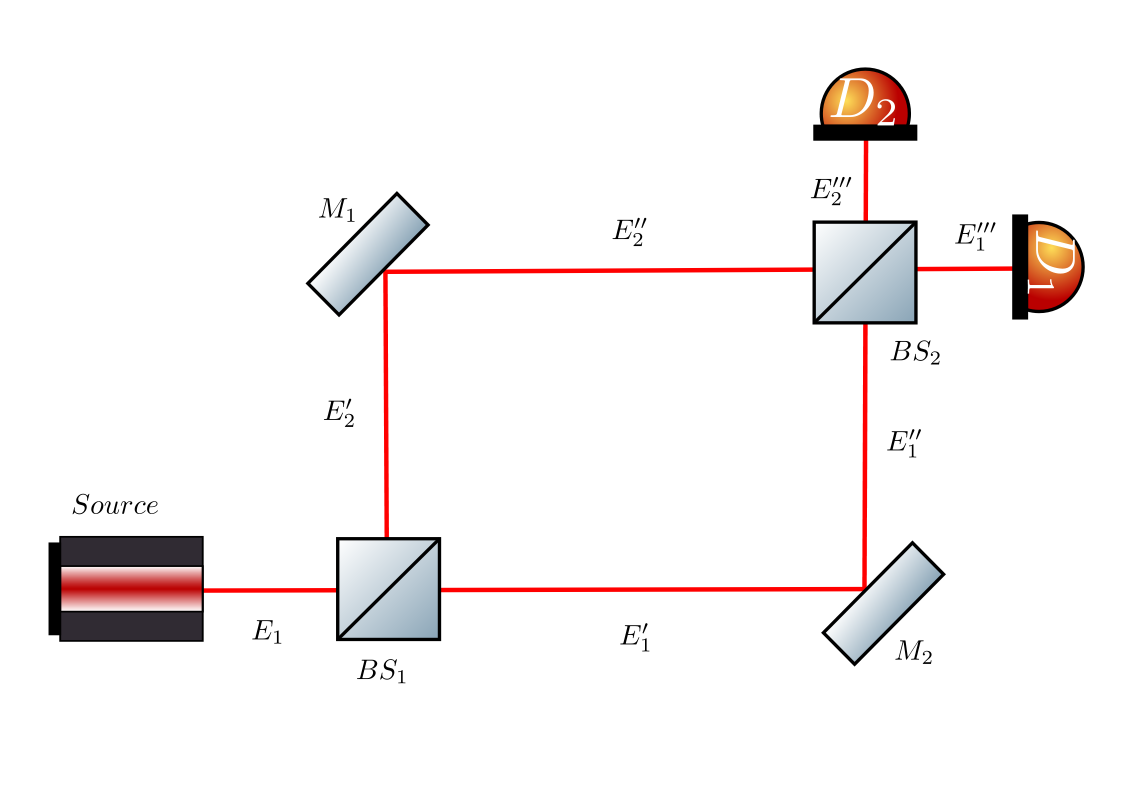
\includegraphics[width=\linewidth]{images/machzenhdercla.png}
\caption{A Mach-Zehnder interferometer.}
\label{fig:classical mach}
\end{figure}



\section{Classical Mach-Zehnder interferometer}

In this section, we study the Mach-Zehnder interferometer in the classical regime. We will denote the classical fields going through the interferometer as it is shown in Fig. \ref{fig:classical mach}. We will follow the approach taken by Loudon \cite{ludon}. Let us consider two lossless beam splitters   $BS_{1}$, $BS_{2}$ with the same reflectivity $\rho$ and transmitivity $\tau$. After the first beam splitter, the electric field $E_{1}$ of the incident beam is split into two beams $E_{1}'$ and $E_{2}'$ written as:

\begin{equation}
E_{1}'=\tau E_{1} ,\qquad E_{2}'=\rho E_{1}.\label{corr1}
\end{equation}

The action of the matrix $M$ representing the mirrors only add a phase $e^{i\gamma_{i}}$, where $i=1,2$. As a second stage, after the light strikes the mirrors $M_{1}$ and $M_{2}$, the electric fields $E_{1}''$ and $E_{2}''$ in each path are:

\begin{equation}
 E_{1}''=e^{i\gamma_{1}}E_{1}', \qquad E_{2}''=e^{i \gamma_{2}}E_{2}'.\label{corr2}
\end{equation}

As a final stage, the fields are recombined in the second beam splitter $BS_{2}$ producing the output fields $E_{1}'''$ and $E_{2}'''$:

\begin{align*}
E_{1}'''=\tau E_{2}'' +\rho E_{1}'', \qquad E_{2}'''=\tau E_{1}'' -\rho E_{2}''.\label{corr} \numberthis
\end{align*}

We can write the output in terms of the input field substituting Eqs. \ref{corr1}, \ref{corr2} in Eq. \ref{corr} as :

\begin{align*}
E_{1}'''&=\tau \rho (e^{i \gamma_{1}}+ e^{i \gamma_{2}})E_{1},\\
E_{2}'''&=(\tau^2 e^{i \gamma_{1}}  -\rho^2 e^{i \gamma_{2}})E_{1}.
 \numberthis
\end{align*}

The intensities at the detectors can be calculated by taking the modulus squared of the fields, where $\delta \gamma=\gamma_{1}-\gamma_{2}$:

\begin{align*}
I_{D_{1}}& \propto \abs{E_{1}}^2 2 |\rho \tau|^2\left[1+\cos(\delta \gamma)\right],\\
I_{D_{2}}& \propto \abs{E_{1}}^2 (|\rho|^4 +|\tau|^4)\left[1-\frac{2 |\rho \tau|^2}{|\rho|^4+|\tau|^4}\cos(\delta \gamma)\right]. \numberthis
\end{align*}

A case of interest occurs whenever $\rho =\tau=\frac{1}{\sqrt{2}}$. In this circumstances the intensities become:

\begin{align*}
I_{D_{1}}  \propto \abs{E_{1}}^2 \frac{1+\cos(\delta \gamma)}{2}, \quad
I_{D_{2}}  \propto \abs{E_{1}}^2 \frac{1-\cos(\delta \gamma)}{2}. \numberthis \label{Intensities}
\end{align*}
 
 If additionally   $\delta \gamma=2 \pi n$ where $n=1,2,3,...$, then $\cos(\delta\gamma )=1$ and the detector $D_{1}$ receives the intensity of the initial beam $I_{D_{1}}\propto \abs{E_{1}}^2$ and $D_{2}$ receives no light $I_{D_{2}}= 0.$


\section{Single-photon Mach-Zehnder interferometer}

In this section, we will study a single-photon Mach-Zehnder interferometer, which will be the main object of concern for the rest of this work. In this part of the analysis, we will assume that the mirrors induce different phases in each path. This is done to account for misalignment in our model. It will be proven in a later chapter that this is equivalent to considering phase-shifters inducing differences in the optical paths. We write the matrix representation of the mirrors as:

\begin{equation}
M_{i}= \begin{pmatrix} 0& e^{i\gamma_{i}} \\ e^{i\gamma_{i}} & 0 \end{pmatrix}, \quad i=1,2.
\end{equation}

and a beam splitter as in Eq. \ref{BS_matrix}. Once we have defined the main elements we can analyze the single-photon Mach-Zehnder interferometer. A single photon state, generated via SPDC, is sent into the horizontal path of the interferometer as input signal. In order to study a general situation, we will consider two different $BS$ in our interferometer. Then, our initial state $\ket{1}$  is transformed by the first $BS$ as:

\begin{align}
\ket{1}\xrightarrow{\text{BS1}}\cos(\theta_{1})\ket{1}+i\sin(\theta_{1})\ket{2}.
\numberthis
\end{align}

 Note that the action of optical elements is local, meaning that the matrix $M_1$ ($M_2$) acts only onto the input state of the mirror$\ket{2}$ ($\ket{1}$). After passing through the first $BS$, the photon encounters a mirror in each path, and then both paths are recombined in the second $BS$, as in Fig. \ref{fig:classical mach}. The whole action of the interferometer on the initial state $\ket{1}$ is then:


\begin{align*}
\ket{1}&\xrightarrow{\text{BS1}}\cos(\theta_{1})\ket{1}+i\sin(\theta_{1})\ket{2}\xrightarrow{\text{Mirrors}}\cos(\theta_{1})e^{i\gamma_{1}}\ket{2}+i\sin(\theta_{1})e^{i\gamma_{2}}\ket{1} \\ &\xrightarrow{\text{BS2}}
 i\left[\cos(\theta_{1})\sin(\theta_{2})e^{i\gamma_{1}}+\cos(\theta_{2})\sin(\theta_{1})e^{i\gamma_{2}}\right]\ket{1}\\&+\left[\cos(\theta_{1})\cos(\theta_{2})e^{i\gamma_{1}}-\sin(\theta_{1})\sin(\theta_{2})e^{i\gamma_{2}}\right]\ket{2}. \numberthis
\end{align*}

The probabilities of detection in either $D_{1}$ and $D_{2}$ are now given by

\begin{align}
P_{D_{1}}=|\cos(\theta_{1})\sin(\theta_{2})+\cos(\theta_{2})\sin(\theta_{1})e^{i(\gamma_{2}-\gamma_{1})}|^{2},\label{newergraph}\\
P_{D_{2}}=|\cos(\theta_{1})\cos(\theta_{2})-\sin(\theta_{1})\sin(\theta_{2})e^{i(\gamma_{2}-\gamma_{1})}|^{2}. \label{newgraph}
\end{align}

If we consider the constraint $\theta_{2}=\frac{\pi}{2}-\theta_{1}$ then $P_{D_{1}}$ reduces to $|1-e^{i(\gamma_{2}-\gamma_{1})}|^{2}$ and $P_{D_{2}}$ reduces to $|1+e^{i(\gamma_{2}-\gamma_{1})}|^{2}$, which we can rewrite as

\begin{equation}
P_{D_{1}}=\frac{1+\cos(\gamma_{2}-\gamma_{1})}{2}, \qquad P_{D_{2}}=\frac{1-\cos(\gamma_{2}-\gamma_{1})}{2}. \label{pp_wheler}
\end{equation}

Perfect alignment means no difference in the optical path, $\gamma_{2}-\gamma_{1}=0$, then the probability to detect a photon in $D_{1}$ is one and in $D_{2}$ is zero, perfectly compatible with the result obtained in the classical case. We expect a similar result because the classical case is nothing but many repetitions of the single-photon phenomenon.

\section[Analysis with phase retarders]{Analysis of a Mach-Zehnder interferometer with additional phase retarders}

The interferometer is an instrument quite hard to align experimentally, in most cases alignment is a little off. We can characterize just how off this alignment is by considering the effects of phase retarders on each arm of the interferometer, after all, misalignment is nothing but differences in the optical path. Those predictions can be compared with the actual interferometer (without phase retarders), a wave retarder's  matrix representation is :


\begin{equation}
 R=\begin
{pmatrix} e^
{i c} & 0\\0& e^
{i k }\end
{pmatrix},
\end{equation}

when placed in the horizontal path $k=0$ and when placed in the vertical $c=0$. Let us see the effect of such an optical device in our setup:

\begin{align*}
\ket{1}&\xrightarrow{\text{BS1}}\cos(\theta_{1})\ket{1}+i\sin(\theta_{1})\ket{2}\\ &\xrightarrow[\text{Retarders}]{\text{Phase}}\cos(\theta_{1})e^{ic}\ket{1}+i\sin(\theta_{1}) e^{ik}\ket{2} \\ &\xrightarrow{\text{Mirrors}} \cos(\theta_{1})e^{i(\frac{\pi}{2}+c)}\ket{2}+i\sin(\theta_{1})\beta e^{i(\frac{\pi}{2}+k)}\ket{1},
\end{align*}

we can stop here by noticing that replacing $\frac{\pi}{2}+k\xrightarrow{}\gamma_{2}$ and  $\frac{\pi}{2}+c\xrightarrow{}\gamma_{1}$,  is the same as using the mirror matrix given by Eq. \ref{mirror} so our model that makes use of this matrix  instead of the more popular mirror matrix with a fixed phase $M=\begin{pmatrix} i & 0\\0& i\end{pmatrix}$, where $i=e^{i \frac{\pi}{2}}=e^{i\gamma}$, has the  effect of a phase retarder included, allowing us to study misalignment. 

\afterpage{\blankpage}

\chapter{ Interaction-free  measurements}


In this chapter, we will explore what is known in the literature as interaction-free measurements. The possibility of performing such kind of measurements was first reported by Elitzur and Vaidman in \cite{Elitzur}. Since then, the topic has awakened a lot of discussion about the non-local nature of quantum theory as well as the philosophical interpretations of quantum mechanics\footnote{ These philosophical discussions will be kept to a minimum in this thesis since they are way more philosophical than physical and highly speculative. Interesting discussions can be found in \cite{paper_vaidman, maudlin}. }. We will now analyze the simplest case proposed by Elitzur and Vaidman.

\section[Elitzur-Vaidman's bomb detector]{Single-photon Mach-Zehnder interferometer with a perfect absorber}

Consider a Mach-Zehnder interferometer where we could or could not place a perfectly absorbent object in one of its paths. Consider also that a single photon is traveling through the interferometer. This system is best known as the Elitzur-Vaidman's bomb detector \cite{Elitzur}. In order to express their ideas in a more dramatic way, Elitzurt and Vaidman proposed that the perfect absorber may be a bomb that is sensitive to the interaction with a single-photon. The bomb is supposed to explode if only a single-photon enters its sensor. An interesting aspect of this experiment is that it exhibits the non-local nature of quantum mechanics, as it allows the possibility of getting knowledge of whether the perfect absorber is in one of the arms of the interferometer performing a measurement without touching it. Yet, Elitzur and Vaidman showed that the single-photon Mach-Zehnder interferometer supplies a mechanism to detect if the bomb was there, without exploding it. They concluded that this can be achieved in, at most, $25\%$ the events.


\begin{figure}[t!]
\centering
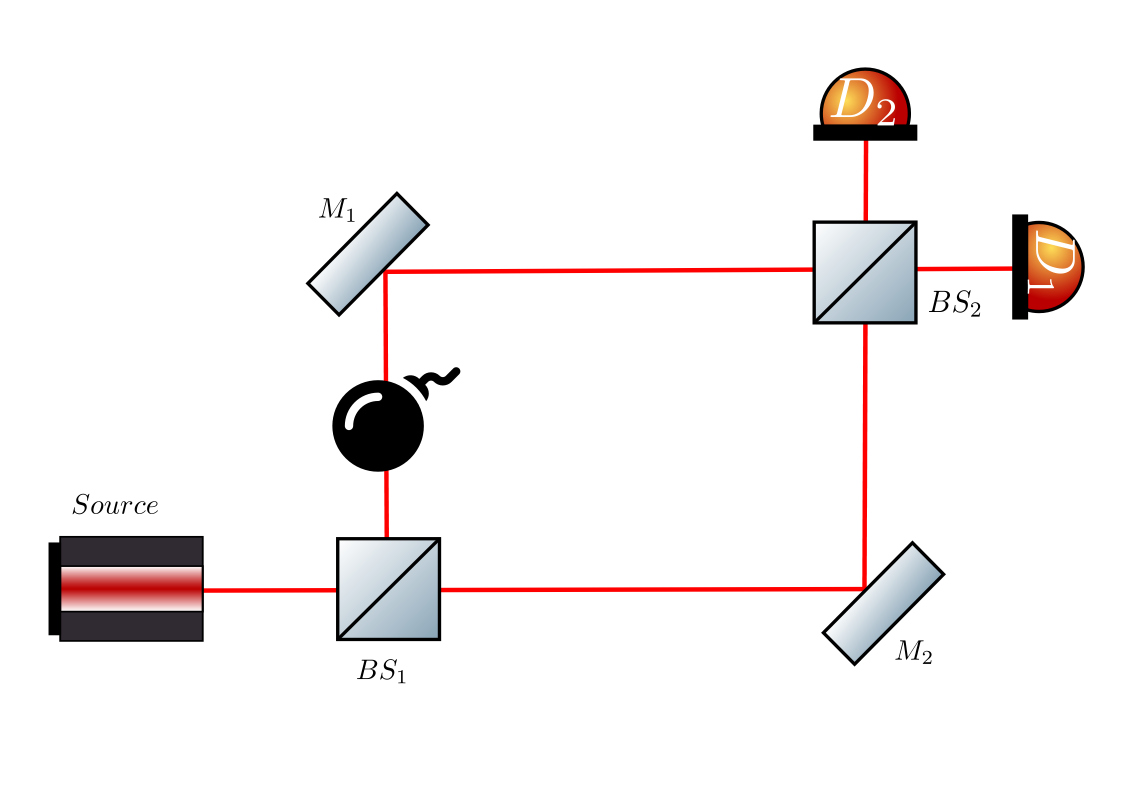
\includegraphics[width=\linewidth]{images/machzenhderbomb.png}
\caption{Elitzur-Vaidman's bomb detector.}
\label{fig:bomb}
\end{figure}

To analyze this system, we will consider the Mach-Zehnder model of section 3.2 but this time having a perfect absorber in its vertical arm,  as Fig. \ref{fig:bomb} shows. We will also consider that once the photon is absorbed, the optical elements of the interferometer do not interact with it any longer. We will denote the state corresponding to an absorbed photon by means of the $\ket{abs}$ vector. Assume a single-photon is pumped in the horizontal input channel of the Mach-Zehnder interferometer. First, the initial state of the system is transformed by the beam splitter $BS_{1}$, into a superposition state of the single photon being transmitted to the horizontal output of $BS_{1}$ and being reflected to the vertical one. Then, the photon could either be absorbed by the bomb if it was traveling towards $M_1$ or be reflected by $M_2$ if it was traveling in the other arm. The mirror $M_{2}$, in turn, transforms the state into the state of the photon being redirected to the beam splitter $BS_{2}$, where it is finally split into the linear combination of being transmitted to detector $D_{2}$ or reflected to detector $D_{1}$. We have 
 
\begin{align*}
\ket{1}&\xrightarrow{\text{BS1}}\cos(\theta_{1})\ket{1}+i\sin(\theta_{1})\ket{2}\\ &\xrightarrow{\text{Bomb}}\cos(\theta_{1})\ket{1}+i\sin(\theta_{1})\ket{abs}\\ &\xrightarrow{\text{Mirrors}}
 i\cos(\theta_{1})\ket{2}+i\sin(\theta_{1})\ket{abs} \\ &\xrightarrow{\text{BS2}}i\cos(\theta_{1})\cos(\theta_{2})\ket{2}-\cos(\theta_{1})\sin(\theta_{2})\ket{1}+i\sin(\theta_{1})\ket{abs}, \numberthis
\end{align*}

where $M_{2}$ is such that $\gamma=\frac{\pi}{2}$, and $\theta_{1}$, $\theta_{2}$ are the parameters in the beam splitter matrix for $BS_{1}$,  $BS_{2}$. The probabilities to be either absorbed or detected at either $D_{1}$ or $D_{2}$ are given by:

\begin{equation}
P_{D_{1}}=\cos^2(\theta_{1}) \sin^2(\theta_{2}),\qquad P_{D_{2}}=\cos^2(\theta_{1}) \cos^2(\theta_{2}),\qquad P_{abs}=\sin^2(\theta_{1}).
\end{equation}

As a particular case, if both, $BS_{1}$ and $BS_{2}$ are $50:50$ beam splitters, i.e where $\theta_{1}=\theta_{2}=\frac{\pi}{4}$, then:

\begin{equation}
P_{D_{1}}=\frac{1}{4},\quad P_{D_{2}}=\frac{1}{4}, \quad P_{abs}=\frac{1}{2}.
\end{equation}



If we detect the photon in $D_{1}$, we get no useful information to conclude about the presence of the bomb, as this result is always obtained in the conventional Mach-Zehnder interferometer. Thus, in $\frac{1}{2}$ of the times, we make a measurement we cannot tell whether the bomb is there or not. In this experiment, the bomb has a $\frac{1}{2}$ probability of exploding by interacting with the photon. Additionally there is a $\frac{1}{2}$ probability that the photon is detected either at $D_{1}$ or $D_{2}$. So fifty percent of the time we have interaction-free measurements, to tell whether an object is there or not we need to consider that if the photon is detected at $D_{2}$, then it indicates that there is an object in one of the arms of the interferometer. However, we cannot distinguish between this case and the previous one section 3.2 from a single event if we detect at $D_{1}$, so $\frac{1}{2}$ of the times we make a measurement we can't tell if a bomb is there or not. Since we are dealing with just one measurement it is not so useful to talk about conditional probabilities such as, 'what is the probability of detecting in $D_{2}$, if the object is not absorbed' in the same way that it is not useful to talk about the probability of having a single dice throw come out as six provided it was not one. However, it is useful to analyze the efficiency of this interferometer, that is just how probable it is for us to realize interaction-free measurements, the efficiency is given by \cite{5}:

\begin{equation}
\eta=\frac{P_{det}}{P_{det}+P_{abs}},
\end{equation}

where $\eta$ is the efficiency, $P_{det}$ is the probability the object is detected, considering lossless optical devices, which we do in this work $P_{det}+P_{abs}=1$ and we have

\begin{equation}
\eta=P_{D_{1}}+P_{D_{2}}.
\end{equation}

For example, in the case, we explored in this section $\eta=\frac{1}{2}$.  Whenever a perfect absorber is in one of the arms of the interferometer, detecting a photon in either $D_1$ or $D_2$ means that the photon did not interact with the bomb. As discussed above, detecting at $D_1$ does not give us information about the presence of the bomb. Since the goal is to determine if the bomb is there, a detection in $D_2$ is an ‘interaction-free measurement’ that confirms the presence of the bomb.
  
\section[Replacing the bomb with an imperfect transmitter]{Replacing the bomb with an imperfect transmitter}

This section is based on the treatment reported by Z. Blanco-Garcia and O. Rosas-Ortiz \cite{zuri,azuri}, and the work by Azuma \cite{Azuma}. 


Let us replace the ``bomb'' from section 4.1 with a semi-transparent object. The absorption and transmission coefficients of such an object will be denoted by $\alpha$ and $\beta$, respectively, satisfying the condition $|\alpha|^2 + |\beta|^2 = 1.$



In the same Horizontal-Vertical basis, our initial state is $\ket{1}$. We will place our imperfect transmitter in the vertical output path of the beam splitter $BS_{1}$ as Fig. \ref{fig:bomb} shows. Our transmitter can either transmit with probability $|\beta|^2$ or absorb with probability $|\alpha|^2$, when a photon in the state $\ket{2}$ travels throught the object, the state transforms as:


\begin{align}
\ket{2}\xrightarrow[\text{Absorber}]{\text{Imperfect}}\alpha \ket{abs} +\beta \ket{2}.
\end{align}

With this information model the experiment. We start out with a photon state at the horizontal entry port of $BS_1$. Then, the initial state is transformed by $BS_{1}$ into a superposition of $\ket{1}$ and $\ket{2}$. The vertical component interacts with the so called by the imperfect transmitter which decomposes the component $\ket{2}$ into a superposition of $\ket{2}$ and $\ket{abs}$ (being transmitted or being absorbed). Afterward, the mirror in each path interchanges $\ket{1}\rightarrow{}\ket{2}$ and vice versa, in this section, we will consider mirrors such that $\gamma=\frac{\pi}{2}$. Finally, the state is recombined in the second beam splitter $BS_{2}$. Mathematically, this process is written as 

\begin{align*}
 \ket{1}&\xrightarrow{\text{BS1}}\cos(\theta_{1})\ket{1}+i\sin(\theta_{1})\ket{2} \\ &\xrightarrow[\text{Absorber}]{\text{Imperfect }}\cos(\theta_{1})\ket{1}+i\sin(\theta_{1})(\alpha \ket{abs} +\beta \ket{2} )
\\ &\xrightarrow{\text{Mirrors}} i\cos(\theta_{1})\ket{2}+i \sin(\theta_{1})\alpha\ket{abs}-\sin(\theta_{1})\beta\ket{1} \\ &\xrightarrow{\text{BS2}} -
(\cos(\theta_{1})\sin(\theta_{2})+\beta \sin(\theta_{1})\cos(\theta_{2}))\ket{1}+ i \alpha \sin(\theta_{1})\ket{abs} \\  & \qquad +i(\cos(\theta_{1})\cos(\theta_{2})-\sin(\theta_{1})\sin(\theta_{2})\beta)\ket{2}. \numberthis
\end{align*}

Then, the probabilities of detection at $D_1$, $D_2$ and absorption of the photon are 
\begin{align}
& P_{D_{1}}=|\cos(\theta_{1})\sin(\theta_{2})+\beta \sin(\theta_{1})\cos(\theta_{2})|^2, \label{eq1}\\
& P_{D_{2}}=|\cos(\theta_{1})\cos(\theta_{2})-\beta \sin(\theta_{1})\sin(\theta_{2})|^2, \\
& P_{abs}=|\alpha \sin(\theta_{1})|^2. \label{eq2}
\end{align}

Again, detection at $D_1$ tells us nothing about the presence of the object. But if we detect at $D_2$ we know that the object was in the vertical arm of the interferometer. Some people argue that this is no longer an interaction-free measurement because the photon may have passed through the semitransparent object, they refer to this kind of setup as 'quantum interrogation' \cite{QI1,QI2}. 


From, now on we will write detection probabilities as $P_{ij}$ where $i=1$ ($i=2$) means that the object was placed just after $BS_1$ in the horizontal (vertical) arm of the interferometer, in previous calculation $i=2$. Subindex $j$ denotes one of the possible outcomes $j=D_{1},D_{2},abs$. In this notation $P_{D_1}= P_{2D_{1}}, ~P_{D_2}= P_{2D_{2}}, ~P_{abs}= P_{2abs} $. 

By locating our imperfect transmitter on the horizontal arm of the interferometer, we obtain:

\begin{align}
P_{1D_{1}}&=|\beta\cos(\theta_{1})\sin(\theta_{2}) +\sin(\theta_{1})\cos(\theta_{2})|^2,\label{eq3} \\
P_{1D_{2}}&=|\sin(\theta_{1})\sin(\theta_{2})-\beta \cos(\theta_{1})\cos(\theta_{2})|^2,\\
P_{1abs}&=|\alpha \cos(\theta_{1})|^2. \label{eq4}
\end{align}



Observe that, in general, the probabilities Eqs. \ref{eq1}-\ref{eq2} are different to those in Eqs. \ref{eq3}-\ref{eq4}. We can consider the difference between them to see when the output depends on the arm in which we place the object.


\begin{align}
P_{1D_{1}}-P_{2D_{1}}=(1-|\beta|^2)\left(\frac{\cos(2 \theta_{1})-\cos(2 \theta_{2})}{2}\right), \\
P_{1D_{2}}-P_{2D_{2}}=(1-|\beta|^2)\left(\frac{\cos(2 \theta_{1})+\cos(2 \theta_{2})}{2}\right).
\end{align}

These expressions tell us how distinguishable these outcomes are.  We can say that the outcome probabilities are the same only the following cases:

\begin{description}

\item[a)] A completely transparent object $|\beta|=1$.

\item[b)] When $\theta_{1}=\theta_{2}=\frac{\pi}{4}$, that is when both $BS_{1}$ and $BS_{2}$ are 50:50 beam splitters.
\end{description}

Finally, we can also obtain an expression for each one of the angles in terms of the probabilities


\begin{align}
\theta_{2}=\displaystyle \frac{\cos^{-1}\left[\frac{(P_{1D_{2}}-P_{2D_{2}})-(P_{1D_{1}}-P_{2D_{1}})}{1-|\beta|^2}\right]}{2},\label{thetasara}\\
\theta_{1}=\displaystyle \frac{\cos^{-1}\left[\frac{(P_{1D_{2}}-P_{2D_{2}})+(P_{1D_{1}}-P_{1D_{1}})}{1-|\beta|^2}\right]}{2}\label{thetasara1},
\end{align}


where $\cos^{-1}(x)$ is the arccosine of $x$. These equations would allow us to set the values of the beam splitters' transmittance and reflectance coefficients in order to obtain specific values of the probabilities of detection $P_{iD_{1}}$, $P_{iD_{2}}$. This fact will serve us to infer, in a series of measurements, some information about the location of the absorber in the interferometer.  

For example, suppose we consider an interferometer such that, if the object is in the horizontal path, then $P_{1D_{2}}=\frac{1}{3} \quad P_{1D_{1}}=\frac{1}{4}$. Correspondingly,  if the object was in the vertical path $P_{2D_{2}}=\frac{1}{4} \quad P_{2D_{1}}=\frac{1}{3}$. Assuming, for instance that the object is characterized by $|\beta|^{2}=0.5$ the expressions \ref{thetasara}-\ref{thetasara1} for the values $\theta_{1},\theta_{2}$ defining the beam splitters' transmitance and reflectance coefficients would yield

\begin{align*}
\theta_{2} \approx \frac{\pi}{5},\qquad \theta_{1} = \frac{\pi}{4}.
\end{align*}

Thus, expressions \ref{thetasara}-\ref{thetasara1} offer the possibility to design interferometers by means of which we could distinguish between the object being placed in one path or the other by measurements and taking the statistics. From the practical point of view, one should also consider the technical difficulties in constructing the very specific beam splitter needed to perform the measurements, we also risk exploding the bomb in the process, as for the previous values of detection probabilities we have $P_{det}=\frac{7}{12}$ and $P_{abs}=\frac{5}{12}$ (so it would not be wise to try and tell in which path the object maybe).
 




\section{Replacing the bomb with a beam splitter}

We will now study the case where we replaced the bomb discussed in section 4.2 with a beam splitter $BS_{o}$. In this case, we will consider imperfect mirrors $M_{1}$ and $M_{2}$ such that $\gamma_{1}$ and $\gamma_{2}$ are arbitrary, i.e, the mirrors, induce arbitrary phases. So we can model misalignments in the interferometer as described in section 3.3.  Likewise  previous cases, we will first consider our imperfect transmitter is placed in the vertical path as shown in Fig. \ref{bs vertical}. As might be inferred from the Figure, the event of the photon being absorbed by the object is now modeled by the photon being reflected by $BS_{o}$ (the photon goes out of the interferometer, and does not interact any longer with the rest of the optical elements).



\begin{figure}[t!]
\centering
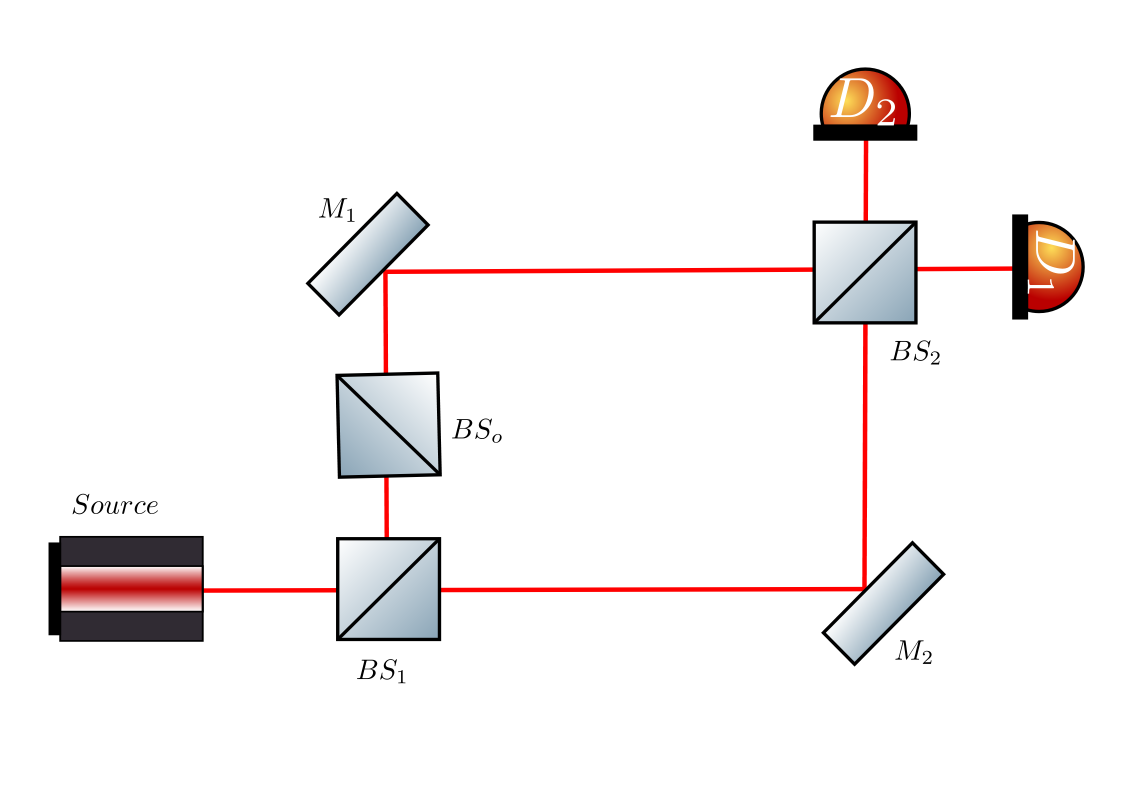
\includegraphics[width=\linewidth,height=7.5 cm]{images/machzenhderbs.png}
\caption{Mach-Zehnder interferometer with a $BS$ as imperfect transmitter.}
\label{bs vertical}
\end{figure}

Thus, let us assume that our imperfect transmitter is a beam splitter $BS_{o}$ whose transmission and reflection coefficients are $\cos(\theta_{o})$ and $i\sin(\theta_{o})$, respectively. When the photon in the state $\ket{2}$ interacts with our imperfect transmitter, its state is transformed as:

\begin{align}
\ket{2}\xrightarrow[\text{transmitter}]{\text{Imperfect}}i\sin(\theta_{o}) \ket{abs} +\cos(\theta_{o}) \ket{2}.
\end{align}

As the reflected photon goes out of the paths of the interferometer, and, thus out of reach of the remaining optical components, it might be considered as if it were absorbed by this component of the device. So, we denote its state by the vector $\ket{abs}$ as in the case of the states of truly absorbed photons of the previous experiments. With that in mind  now our model is an analogous form to those cases of the previous sections.

Assuming the photon enters the interferometer though the horizontal channel, i.e being in the initial state $\ket{1}$, The evolution of the state goes as follows:



\begin{align*}
\ket{1}&\xrightarrow{\text{BS1}}\cos(\theta_{1})\ket{1}+i\sin(\theta_{1})\ket{2}\\
&\xrightarrow{\text{BSo}}\cos(\theta_{1})\ket{1}+i\sin(\theta_{1})\left[\cos(\theta_{o})\ket{2}+i\sin(\theta_{o})\ket{abs}\right]\\ &\xrightarrow{\text{Mirrors}} \cos(\theta_{1})e^{i\gamma_{1}}\ket{2}+i\sin(\theta_{1})\cos(\theta_{o})e^{i\gamma_{2}}\ket{1}-\sin(\theta_{1})\sin(\theta_{o})\ket{abs}\\ &\xrightarrow{\text{BS2}}\cos(\theta_{1})e^{i\gamma_{1}}\left[\cos(\theta_{2})\ket{2}
+i\sin(\theta_{2})\ket{1}\right]+i\sin(\theta_{1})\cos(\theta_{o})e^{i\gamma_{2}}\\
& \qquad \times \left[\cos(\theta_{2})\ket{1}+i\sin(\theta_{2})\ket{2}\right]-\sin(\theta_{1})\sin(\theta_{o})\ket{abs}\\
& \qquad =(\cos(\theta_{1})e^{i\gamma_{1}}\cos(\theta_{2})-\sin(\theta_{1})\sin(\theta_{2})\cos(\theta_{o})e^{i\gamma_{2}})\ket{2}-\sin(\theta_{1})\sin(\theta_{o})\ket{abs}\\ & \qquad +(i\cos(\theta_{1})\sin(\theta_{2})e^{i\gamma_{1}}+
 i \sin(\theta_{1})\cos(\theta_{o})\cos(\theta_{2})e^{i\gamma_{2}})\ket{1}.\numberthis
\end{align*}
The detection probabilities can now be readily written:
\begin{align*}
 P_{2D_{1}}&=|\cos(\theta_{1})\sin(\theta_{2})+ e^{i(\gamma_{2}-\gamma_{1})}\cos(\theta_{o}) \sin(\theta_{1})\cos(\theta_{2})|^2,\\
 P_{2D_{2}}&=|\cos(\theta_{1})\cos(\theta_{2})- e^{i(\gamma_{2}-\gamma_{1})}\cos(\theta_{o}) \sin(\theta_{1})\sin(\theta_{2})|^2,\\
 P_{2abs}&=|\sin(\theta_{o}) \sin(\theta_{1})|^2. \numberthis \label{ajuste}
\end{align*}
\begin{figure}[t!]
\centering
\begin{subfigure}[b]{0.45\linewidth}
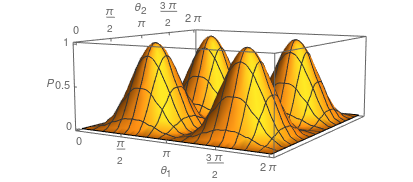
\includegraphics[width=\linewidth,height=2.8 cm]{images/P1abs.png}
\caption{$P_{2abs}$}
\label{fig:BS2}
\end{subfigure}
\begin{subfigure}[b]{0.45\linewidth}
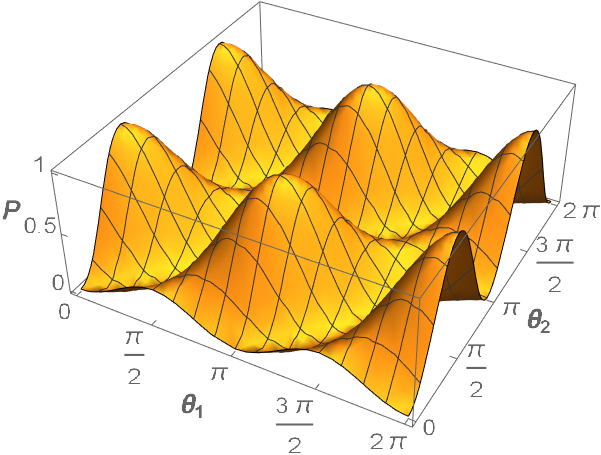
\includegraphics[width=\linewidth,height=2.8 cm]{images/P1d1.png}
\caption{$P_{2D_{1}}$}
\label{fig:westminster_aerea}
\end{subfigure}
\begin{subfigure}[b]{0.45\linewidth}
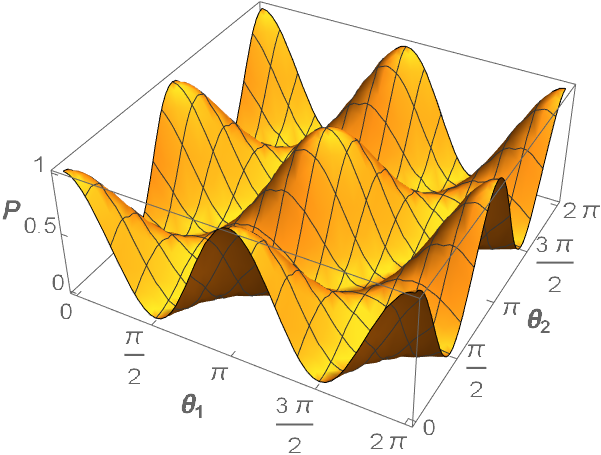
\includegraphics[width=\linewidth,height=2.8 cm]{images/P1d2.png}
\caption{$P_{2D_{2}}$}
\label{fig:BS2}
\end{subfigure}
\caption{Probability distributions of detection and absorption of the photon with the imperfect absorber placed in the vertical path. In these plots $\theta_{o}=\frac{\pi}{3}$ and $\gamma_{2}-\gamma_{1}=\pi$, subfigure (a) corresponds to $P_{2abs}$, (b) to $P_{2D_{1}}$ and (c) to $P_{2D_{2}}$.}
\label{P_bs}
\end{figure}
It is worthwhile noting that $P_{2D_{1}}$ and $P_{2D_{2}}$ do not depend on $\gamma_{1}$ and $\gamma_{2}$ independently but only on the difference $\gamma_{2}-\gamma_{1}$ meaning that the detection probabilties are only sensitive to the relative phases introduced by the mirrors. Adittionally, as it might be expected the absortion probability depends only on the parameters of $BS_{1}$ and $BS_{o}$.

We show the plots for the detection probabilities $P_{2abs}$, $P_{2D_{1}}$ and $P_{2D_{2}}$ in Fig. \ref{P_bs}, as functions of $\theta_{1}$ and $\theta_{2}$ for the particular values of $\theta_{o}=\frac{\pi}{3}$ and $\gamma_{2}-\gamma_{1}=\pi$. There we can see the oscilatory behavious in both parameters:


\begin{figure}[t!]
\centering
\begin{subfigure}[b]{0.4\linewidth}
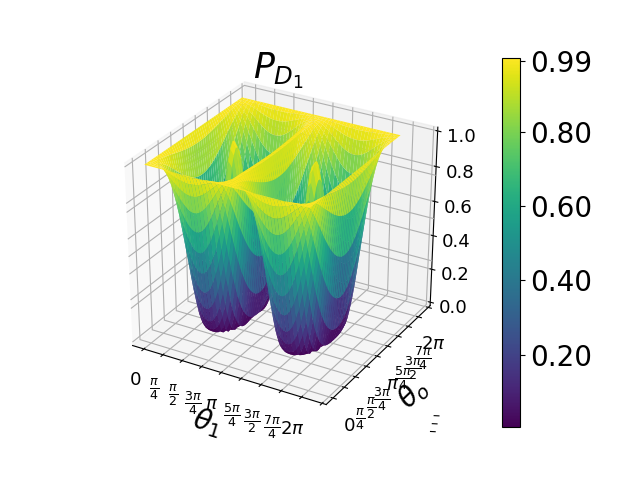
\includegraphics[width=\linewidth]{images/PD1_BS_v.png}
\caption{$P_{2abs}$}
\label{fig:BS2}
\end{subfigure}
\begin{subfigure}[b]{0.4\linewidth}
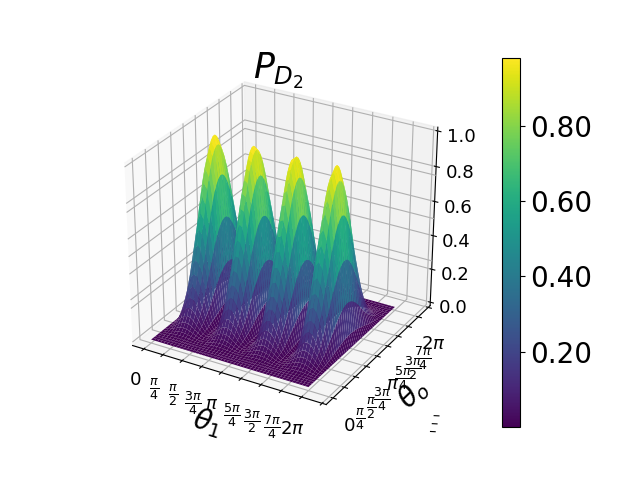
\includegraphics[width=\linewidth]{images/PD2_BS_v.png}
\caption{$P_{2D_{1}}$}
\label{fig:westminster_aerea}
\end{subfigure}
\begin{subfigure}[b]{0.4\linewidth}
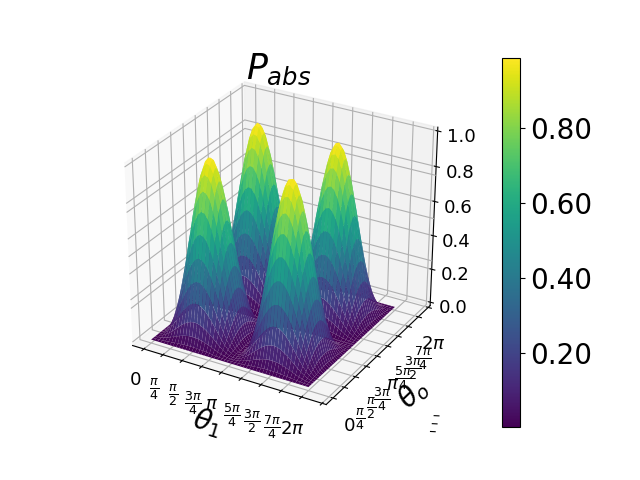
\includegraphics[width=\linewidth]{images/PAbs_BS_v.png}
\caption{$P_{2D_{2}}$}
\label{fig:BS2}
\end{subfigure}
\caption{Probability distributions of detection and absorption of the photon with the imperfect absorber placed in the vertical path. In these plots $\theta_{2}=\frac{\pi}{2}-\theta_{1}$ and $\gamma_{2}-\gamma_{1}=0$, subfigure (a) corresponds to $P_{2abs}$, (b) to $P_{2D_{1}}$ and (c) to $P_{2D_{2}}$.}
\label{P_bs_constraint}
\end{figure}


The above figure Fig. \ref{P_bs} shows probabilities for all possible values of the beam splitter, however, from Eqs.\ref{newergraph}-\ref{newgraph}, we see that not for all values of $\theta_{1}$ and $\theta_{2}$, we can be sure of the output of the interferometer when no object is present, which is a key feature of the Elitzur-Vaidman bomb tester that allows to tell if the bomb is there from just one measurement. In order to have that feature we implement the constraint $\theta_{2}=\frac{\pi}{2}-\theta_{1}$. Using this we generated the plots in Fig. \ref{P_bs_constraint}.
\begin{figure}[t!]
\centering
\begin{subfigure}[b]{0.45\linewidth}
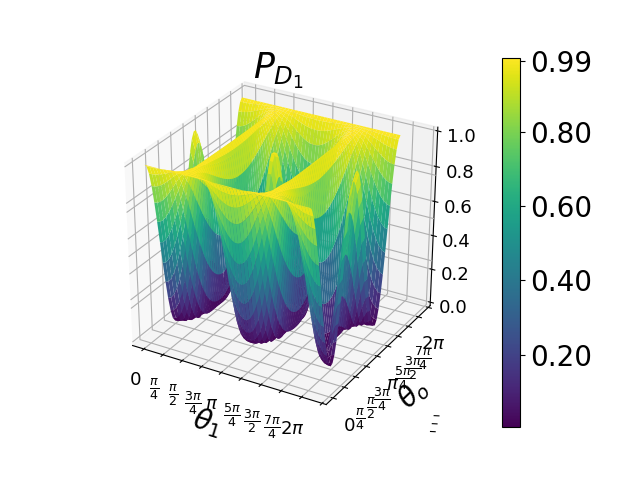
\includegraphics[width=\linewidth]{images/PD1_BS_h.png}
\caption{$P_{1abs}$}
\label{fig:BS1}
\end{subfigure}
\begin{subfigure}[b]{0.45\linewidth}
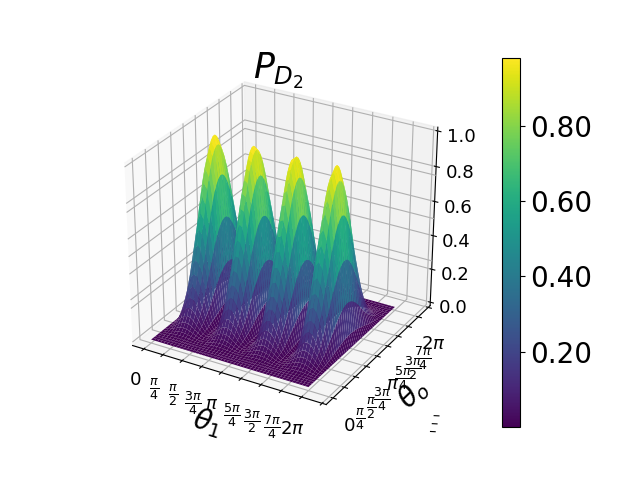
\includegraphics[width=\linewidth]{images/PD2_BS_h.png}
\caption{$P_{1D_{1}}$}
\label{fig:westminster_aerea}
\end{subfigure}
\begin{subfigure}[b]{0.45\linewidth}
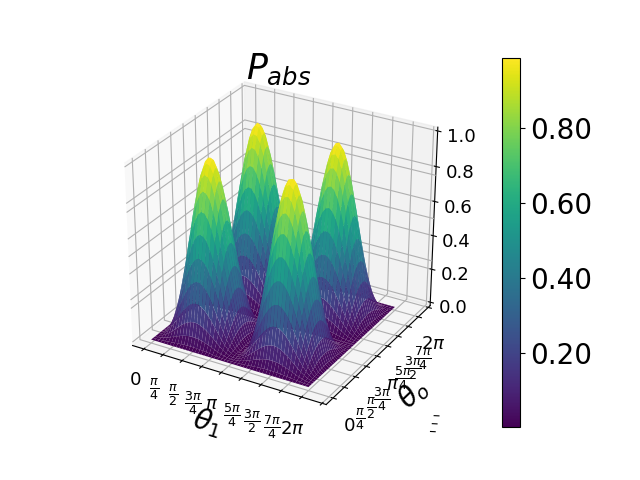
\includegraphics[width=\linewidth]{images/PAbs_BS_v.png}
\caption{$P_{1D_{2}}$}
\label{fig:BS1}
\end{subfigure}
\caption{Probability distributions of detection and absorption of the photon with the imperfect absorber placed in the horizontal path. In these plots $\theta_{2}=\frac{\pi}{2}-\theta_{1}$ and $\gamma_{2}-\gamma_{1}=0$, subfigure (a) corresponds to $P_{1abs}$, (b) to $P_{1D_{1}}$ and (c) to $P_{1D_{2}}$.}
\label{P_bs2}
\end{figure}

One ought to be careful when interpreting these plots, since one may think the values where the probability is one in this plot may be good bomb detectors, but in fact, most of them just correspond to the photon guided by mirrors. 

 

Repeating the same calculation with the beam splitter $BS_{o}$ in the horizontal path we obtain the following detection probabilities



\begin{align}
P_{1D_{1}}&=|e^{i(\gamma_{1}-\gamma_{2})}\cos(\theta_{1})\sin(\theta_{2})\cos(\theta_{o})+ \sin(\theta_{1})\cos(\theta_{2})|^2, \\
P_{1D_{2}}&=|\cos(\theta_{1})\cos(\theta_{o})\cos(\theta_{2})e^{i(\gamma_{1}-\gamma_{2})}- \sin(\theta_{1})\sin(\theta_{2})|^2,\\
P_{1abs}&=|\sin(\theta_{o}) \cos(\theta_{1})|^2 .
\end{align}

which are shown graphically in Fig. \ref{P_bs2} as functions of $\theta_{1}$ and $\theta_{o}$, for the same value of  $\gamma_{2}-\gamma_{1}$ than those of Fig. \ref{P_bs_constraint}. We can see they are quite different except for $P_{D_{2}}$ which is the same (the equations become the same under the constraint $\theta_{2}=\frac{\pi}{2}-\theta_{1}$), valleys in one are hills on the other and one the reasons is that we are always launching the incident photon from the same input channel so that the initial conditions are not symmetrical.




Our results are totally consistent with those reported in \cite{zuri,azuri} by taking $\beta=\cos(\theta_{o})$, $\alpha=i \sin(\theta_{o})$ and $\gamma_{2}-\gamma_{1}=0$. One of the advantages of this setup is that the ``absorbed'' photon, is not really absorbed but redirected through another path and can be monitored as well, by a third detector, say $D_{abs}$, enabling, thus the possibility of correlating the absorption and detection probabilities.

\section{Replacing the bomb with $N$ beam splitters }





In this section, we analyze the case in which an array of $N$ beam splitters are placed along one path of the interferometer (see figure \ref{N_bs}). Let us denote the beam splitters in this array by $BS_{i}$, where $i=1,2,3,4,5,...,N+2$. Assuming that the reflected photon in either beam splitter $BS_{i}$ is ``absorbed'', we have that, the state of the photon initially in the state $\ket{2}$ is transformed into

\begin{align}
BS_{3}\ket{2}=\cos(\theta_{3})\ket{2}+i\sin(\theta_{3})\ket{abs}.
\end{align}

The next beam splitter only acts on the transmitted photon state, since, as explained in the previous section, if the photon is reflected then it goes out of the interferometer and does not interact with the optical elements any longer:
\begin{align}
BS_{4}(\cos(\theta_{3})\ket{2}+i\sin(\theta_{3})\ket{abs})&=\cos(\theta_{3})BS_{4}\ket{2}+i\sin(\theta_{3})\ket{abs},\\
BS_{4}BS_{3}\ket{2}&=\cos(\theta_{3})\cos(\theta_{4})\ket{2}+i A_{2}\ket{abs}.
\end{align}
where $A_{2}$ is the composed absorption coefficient for a two beam splitter array. The action of the rest of the beam splitters are equivalent
\begin{equation}
BS_{5}BS_{4}BS_{3}\ket{2}=\cos(\theta_{3})\cos(\theta_{4})\cos(\theta_{5})\ket{2}+iA_{3}\ket{abs},
\end{equation}
\begin{figure}[t!]
\centering
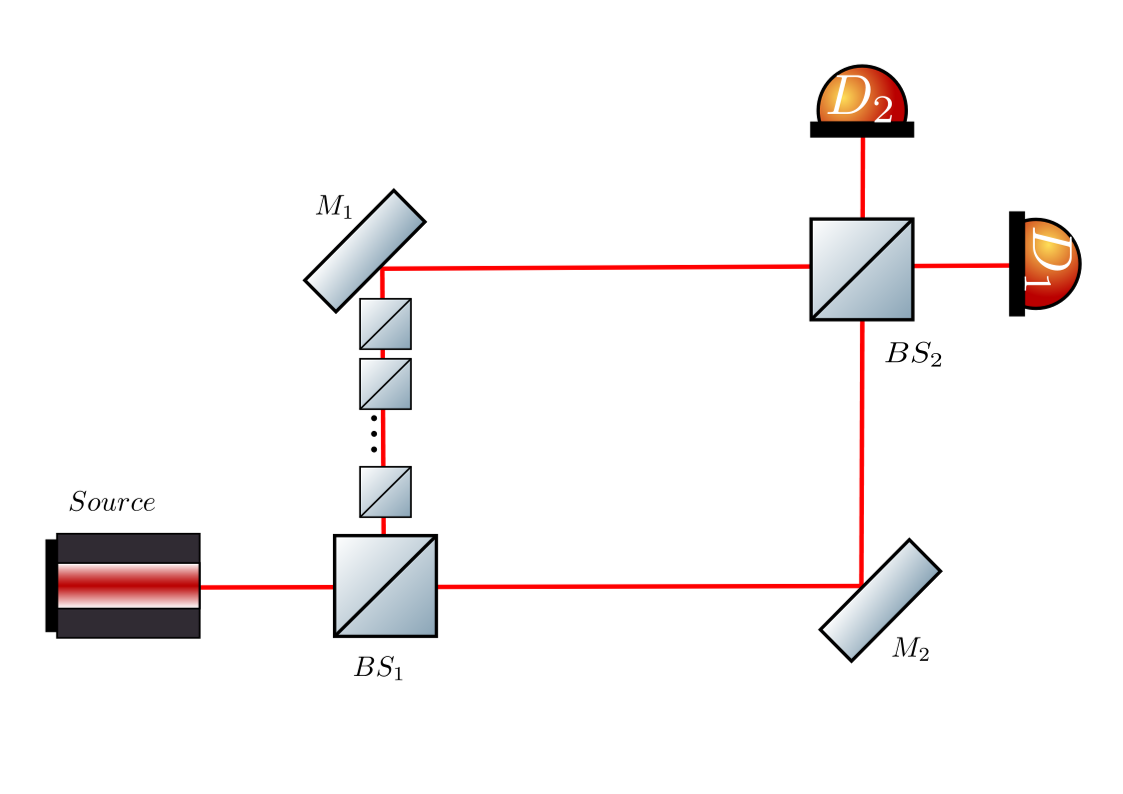
\includegraphics[width=\linewidth,height=8 cm]{images/machzenhderBSS.png}
\caption{Mach-Zehnder with $N$ $BS$ as imperfect transmitter.}
\label{N_bs}
\end{figure}

where $A_{3}$ is the absorption coefficient of the 3-BS array. Finally, for the  $N$ $BS$ array we have:

\begin{align*}
BS^{N}\ket{2}=BS_{N}...BS_{3}\ket{2}=\cos(\theta_{3})\cos(\theta_{4})\cos(\theta_{5})....\cos(\theta_{N})\ket{2} +i A_{N}\ket{abs}. \numberthis
\end{align*}

We can obtain $A_{N}$ by considering that everything that if the photon is not transmitted then it will be ``absorbed":

\begin{align}
BS^{N}\ket{2}&=\prod_{i=3}^{N+2} \cos(\theta_{i})\ket{2}+i A_{N} \ket{abs},\\
A_{N}&=\sqrt{1-\prod_{i=3}^{N+2}\cos^2(\theta_{i})}.
\end{align}

Following a similar procedure, we could obtain a similar result if the $N$ $BS$ array is in the other arm of the interferometer, namely

\begin{align}
BS^{N}\ket{1}&=\prod_{i=3}^{N+2} \cos(\theta_{i})\ket{1}+i \sqrt{1-\prod_{i=3}^{N+2}\cos^2(\theta_{i})} \ket{abs}
\end{align}
 We now use this $N$ $BS$ array to model the imperfect absorber, we can calculate the evolution of a photon initially in state $\ket{1}$ through the interferometer, passing the set of $N$ beam splitters that replaced the bomb (placed in the vertical arm just after $BS_1$), being reflected by $M_1$ and $M_2$, recombined in $BS_2$ and finally going directly to detectors $D_1$ and $D_2$ as: 


\begin{align*}
\ket{1}&\xrightarrow{\text{BS1}}\cos(\theta_{1})\ket{1}+i\sin(\theta_{1})\ket{2}\\ &\xrightarrow{{BS^{N}}}\cos(\theta_{1})\ket{1}+i\sin(\theta_{1})\prod_{i=3}^{N+2} \cos(\theta_{i})\ket{2}-\sin(\theta_{1})\sqrt{1-\prod_{i=3}^{N+2}\cos^2(\theta_{i})}\ket{abs} \\ & \xrightarrow{{Mirrors}}\cos(\theta_{1})  e^{i \gamma_{1}}\ket{2}+i\sin(\theta_{1})\prod_{i=3}^{N+2} \cos(\theta_{i}) e^{i \gamma_{2}}\ket{1}\\
& \qquad -\sin(\theta_{1})\sqrt{1-\prod_{i=3}^{N+2}\cos^2(\theta_{i})}\ket{abs} \\ & \xrightarrow{{BS2}}(\cos(\theta_{1})\cos(\theta_{2})e^{i \gamma_{1}}-\sin(\theta_{1})\sin(\theta_{2})e^{i \gamma_{2}}\prod_{i=3}^{N+2} \cos(\theta_{i}))\ket{2}\\ & \qquad + i(\cos(\theta_{1})\sin(\theta_{2})e^{i \gamma_{1}}+\cos(\theta_{2})\sin(\theta_{1})e^{i \gamma_{2}}\prod_{i=3}^{N+2} \cos(\theta_{i}))\ket{1}\\ & \qquad -\sin(\theta_{1})\sqrt{1-\prod_{i=3}^{N+2}\cos^2(\theta_{i})}\ket{abs}.
\end{align*}
 
The probabilities of detection at each of the detectors and the probability of absorption are given by:

\begin{align}
P_{2D_{1}}&=|\cos(\theta_{1})\sin(\theta_{2})+\cos(\theta_{2})\sin(\theta_{1})e^{i (\gamma_{2}-\gamma_{1})}\prod_{i=3}^{N+2} \cos(\theta_{i})|^2,\\
P_{2D_{2}}&=|\cos(\theta_{1})\cos(\theta_{2})-\sin(\theta_{1})\sin(\theta_{2})e^{i (\gamma_{2}-\gamma_{1})}\prod_{i=3}^{N+2} \cos(\theta_{i})|^2,\\
P_{2abs}&=\sin^2(\theta_{1})\left(1-\prod_{i=3}^{N+2}\cos^2(\theta_{i})\right).
\end{align}


To know whether the array of beam splitters is present, placed, or not, is no different from the previous sections as this case would simply correspond to $\beta=\prod_{i=3}^{N+2} \cos(\theta_{i})$.


\section{A time-dependent transmitter}

In this section, we will consider a time-dependent transmitter by substituting the bomb in the Elitzur-Vaidman experiment with an object whose transmission and absorption coefficients depend on time. This object will be an optical chopper whose time dependence is piecewise. Let us begin by analyzing the optical chopper as a perfect absorber.

\subsection{Replacing the bomb with an optical chopper }
 

An optical chopper is a device that periodically interrupts the transit of a light beam. It usually consists of a disk with dents or gaps that rotates to a certain frequency. The presence of a chopper interrupting the passing of light can be modeled as an object whose coefficient of transmission  varies as a square wave  

\begin{equation}
f(t)=\frac{\mathrm{sgn}(\sin(wt))+1}{2},
\end{equation}

 where $\omega$ is the angular frequency of the optical chopper multiplied by the number of ``hole-material" pairs that we assume are the same size.

 \begin{figure}[h!]
\centering
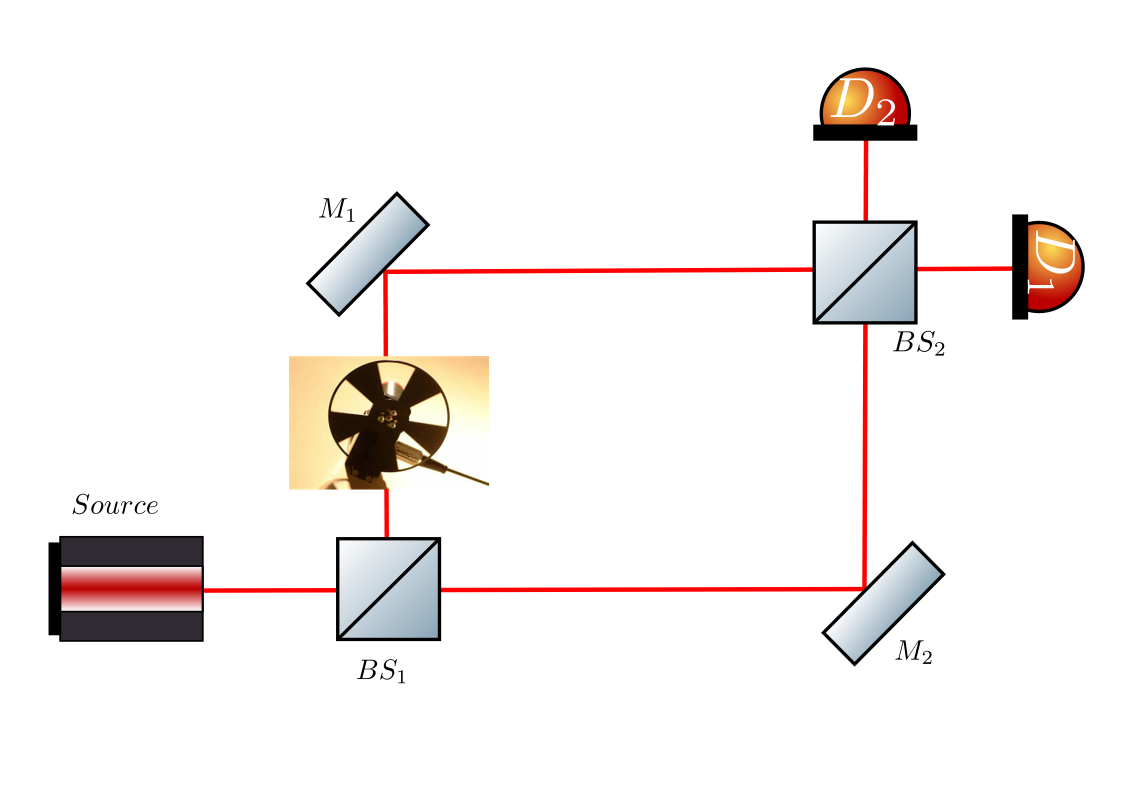
\includegraphics[width=\linewidth]{images/machzenhderchopper.png}
\caption{Mach-Zehnder interferometer with an optical chopper as an imperfect absorber.}
\label{chopper}
\end{figure}

In our model, we will ignore diffraction effects. As a consequence, the transmission coefficient of consecutive optical choppers becomes the product of square waves, and products of square waves are again a square wave. In this form modeling, an array of optical choppers would be equivalent to model one with an effective frequency and duty-cycle. In this section, we consider the Elitzur-Vaidman bomb experiment with a chopper replacing the bomb, see Fig. \ref{chopper}, the chopper will introduce a piecewise time dependence of the transmission coefficient. Leading to two alternating probability distributions.


The optical chopper will be represented by an operator $C_{i}$, where $i$ is the path where the chopper is placed. In our basis (where $i=1,2$):

\begin{equation}
C_{i}\ket{i}=f(t)\ket{i}.
\end{equation}

As we are modeling the gap in the chopper as a transparent object, the operator $C_i$ is unitary in a complete hole-material cycle.  This is indeed fulfilled as the square of the sign function is always one.


Thus $C_{i}$ is a unitary matrix whenever the sine is in the positive semi-cycle, and it becomes null in the negative one. That happens because in the negative semi-cycle we have total absorption of light. The absorption coefficient would  be:  

\begin{align}
 \alpha=1-f,\qquad \alpha=\frac{1-\mathrm{sgn}(\sin(wt))}{2}.
\end{align}

Next, we will analyze a Mach-Zehnder interferometer using a chopper as a time-dependent absorber. The chopper will be placed on the vertical path, while the photon enters the interferometer through the horizontal path. The initial state $\ket{\psi}=\ket{1}$ of the pumping photon transforms in the following way:



\begin{align*}
\ket{1}&\xrightarrow{\text{BS1}}\cos(\theta_{1})\ket{1}+i\sin(\theta_{1})\ket{2}\\ &\xrightarrow{\text{Chopper}}\cos(\theta_{1})\ket{1}+i\sin(\theta_{1})f(t)\ket{2}+i\sin(\theta_{1})\alpha\ket{abs}\\ &\xrightarrow{\text{Mirrors}} \cos(\theta_{1})e^{i\gamma_{1}}\ket{2}+i\sin(\theta_{1})f(t) e^{i\gamma_{2}}\ket{1}+i\sin(\theta_{1})\alpha\ket{abs}\\& \xrightarrow{\text{BS2}}\cos(\theta_{1})e^{i\gamma_{1}}\left[\cos(\theta_{2})\ket{2}+i\sin(\theta_{2})\ket{1}\right]\\
&\qquad +i\sin(\theta_{1})e^{i\gamma_{2}}f(t)\left[\cos(\theta_{2})\ket{1}+i\sin(\theta_{2})\ket{2}\right]+i\sin(\theta_{1})\alpha\ket{abs}\\
&\qquad  = i\left[e^{i\gamma_{1}}\cos(\theta_{1})\sin(\theta_{2})+f(t) e^{i\gamma_{2}}\sin(\theta_{1})\cos(\theta_{2})\right]\ket{1}+\left[ \cos(\theta_{1})\cos(\theta_{2}) e^{i\gamma_{1}} \right. \\&\qquad  \left.  -\sin(\theta_{1})\sin(\theta_{2})f(t) e^{i \gamma_{2}} \right]\ket{2}+i\sin(\theta_{1})\alpha\ket{abs}. \numberthis
\end{align*}


\begin{comment}
A plot for the detection probabilities is shown in Fig. \ref{Pchopper}. As we mentioned before, the system is alternating between two probability distributions. We can see those for each of the possible states in the figure. It is worth noting that the absorption graph alternates between the one shown and no absorption:



\begin{figure}[t!]
\centering
\begin{subfigure}[b]{0.45\linewidth}
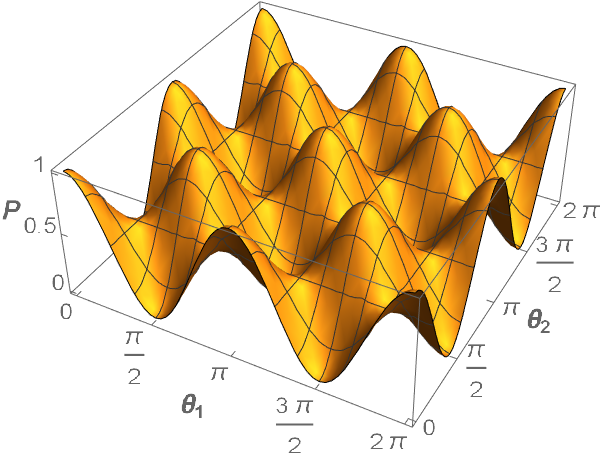
\includegraphics[width=\linewidth,height=3 cm]{images/Pc2D22.png}
\caption{$P_{2D_{2}}$ in the second cycle}
\label{fig:BS1}
\end{subfigure}
\begin{subfigure}[b]{0.45\linewidth}
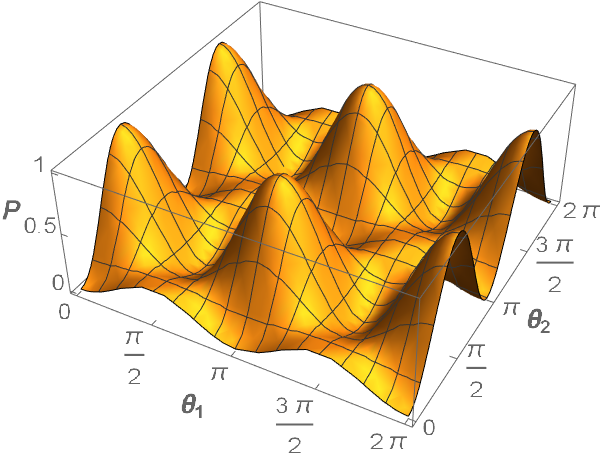
\includegraphics[width=\linewidth,height=3 cm]{images/Pc2D11.png}
\caption{$P_{2D_{1}} $ in the first cycle}
\label{fig:westminster_aerea}
\end{subfigure}
\begin{subfigure}[b]{0.45\linewidth}
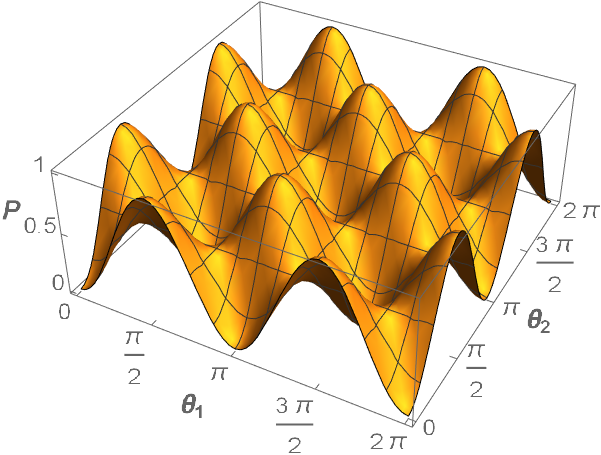
\includegraphics[width=\linewidth,height=3 cm]{images/Pc2D12.png}
\caption{$P_{2D_{1}} $ in the second cycle }
\label{fig:BS1}
\end{subfigure}
\begin{subfigure}[b]{0.45\linewidth}
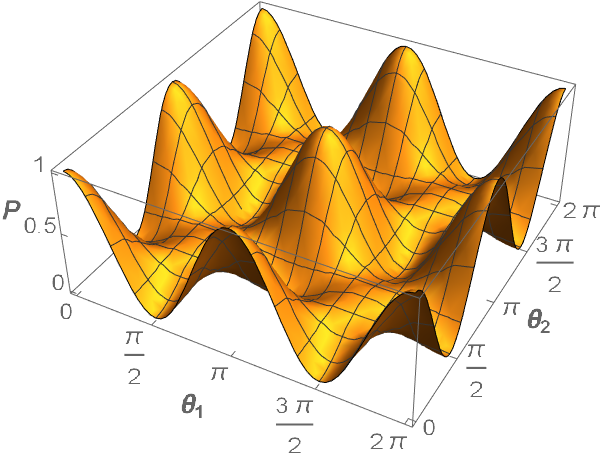
\includegraphics[width=\linewidth,,height=3 cm]{images/Pc2D21.png}
\caption{$P_{2D_{2}}$ in the first cycle }
\label{fig:BS1}
\end{subfigure}
\begin{subfigure}[b]{0.45\linewidth}
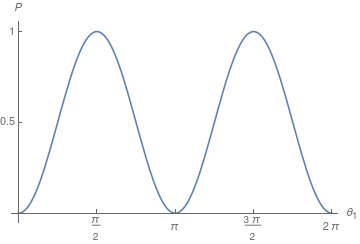
\includegraphics[width=\linewidth,height=3 cm]{images/Pc2Abs.png}
\caption{$P_{2abs}$}
\label{fig:BS1}
\end{subfigure}

\caption{Probability distributions of detection and absorption of the photon at detectors $D_{1}$ and $D_{2}$ with an optical chopper whose solid material is totally absorbent  placed in the vertical path. In these plots  $\gamma_{2}-\gamma_{1}=\frac{\pi}{2}$, subfigure (a) corresponds to $P_{2D_{2}}$ in the second cycle, (b) to $P_{2D_{2}}$ in the first cycle, (c) and (d) to $P_{2D_{1}}$ in the second and first cycle, respectively, and (e) to $P_{2abs}$.}
\label{Pchopper}
\end{figure}

\end{comment}

The corresponding detection probability distributions can be readily written:

\begin{align}
&P_{2D_{1}}=|e^{i\gamma_{1}}\cos(\theta_{1})\sin(\theta_{2})+f(t) e^{i\gamma_{2}}\sin(\theta_{1})\cos(\theta_{2})|^2,\\
&P_{2D_{2}}=|\cos(\theta_{1})\cos(\theta_{2})e^{i\gamma_{1}}- f(t) \sin(\theta_{1})\sin(\theta_{2})e^{i\gamma_{2}}|^2,\\
&P_{2abs}=|\alpha \sin(\theta_{1})|^2,
\end{align}

which can conveniently be rewritten as:
\begin{align*}
 P_{2D_{1}}=&\cos^2(\theta_{1})\sin^2(\theta_{2})+f^2 \sin^2(\theta_{1})\cos^2(\theta_{2})\\
&+\frac{f \sin(2\theta_{1})\sin(2\theta_{2})\cos(\gamma_{1}-\gamma_{2})}{2}, \numberthis{}\\
P_{2D_{2}}=&\cos^2(\theta_{1})\cos^2(\theta_{2})+ f^2 \sin^2(\theta_{1})\sin^2(\theta_{2})\\
&-\frac{f \sin(2\theta_{1})\sin(2\theta_{2})\cos(\gamma_{1}-\gamma_{2})}{2},\numberthis{} \\
 P_{2abs}=&\alpha^2 \sin^2(\theta_{1}).\numberthis{}
\end{align*}

By the same procedure having the chopper in the horizontal path, one can obtain the following results \begin{comment}
which are shown in Fig. \ref{P2chopper}, for each of the possible states of the system
 
\begin{figure}[h!]
\centering

\begin{subfigure}[b]{0.35\linewidth}
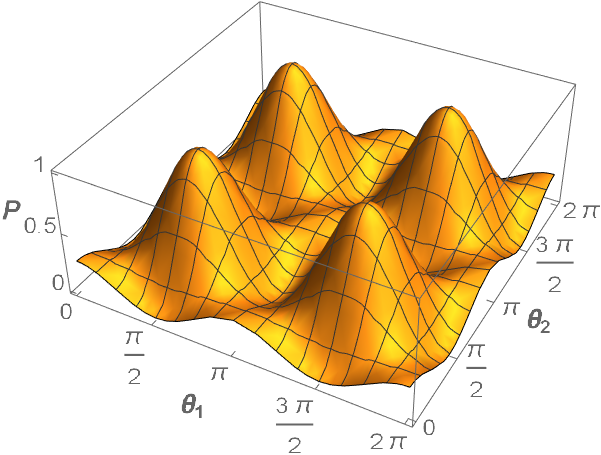
\includegraphics[width=\linewidth,height=3 cm]{images/Pc1D21.png}
\caption{$P_{1D_{2}}$ in the first cycle }
\label{fig:BS1}
\end{subfigure}
\begin{subfigure}[b]{0.35\linewidth}
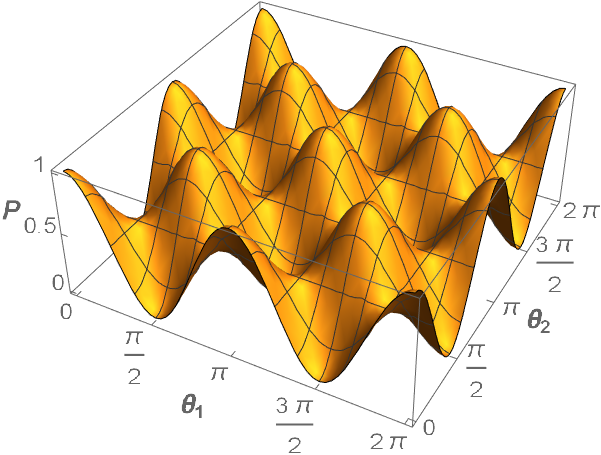
\includegraphics[width=\linewidth,height=3 cm]{images/Pc1D22.png}
\caption{$P_{1D_{2}}$ in the second cycle}
\label{fig:BS1}
\end{subfigure}
\begin{subfigure}[b]{0.35\linewidth}
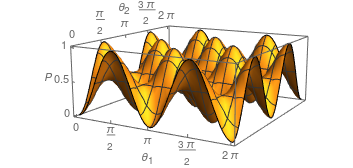
\includegraphics[width=\linewidth,height=3 cm]{images/Pc1D11.png}
\caption{$P_{1D_{1}} $ in the first cycle}
\label{fig:westminster_aerea}
\end{subfigure}
\begin{subfigure}[b]{0.35\linewidth}
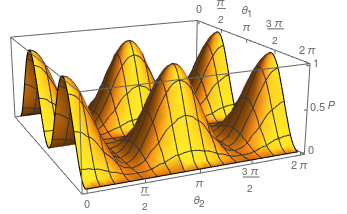
\includegraphics[width=\linewidth,height=3 cm]{images/Pc1D12.png}
\caption{$P_{1D_{1}} $in the second cycle }
\label{fig:BS1}
\end{subfigure}
\begin{subfigure}[b]{0.35\linewidth}
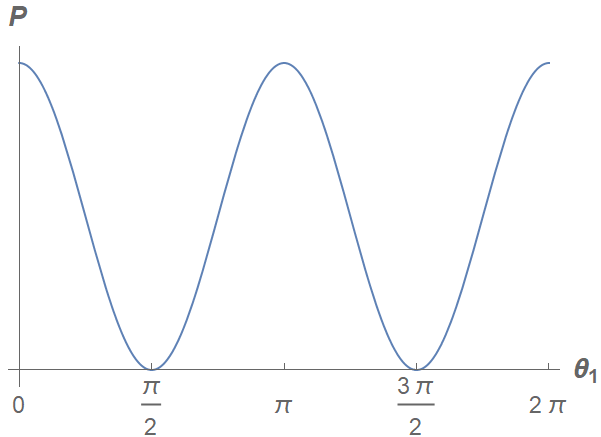
\includegraphics[width=\linewidth,height=3 cm]{images/Pc1Abs.png}
\caption{$P_{1abs}$}
\label{fig:BS1}
\end{subfigure}
\caption{Probability distributions of detection and absorption of the photon at detectors $D_{1}$ and $D_{2}$ with an optical chopper whose solid material is totally absorbent  placed in the horizontal path. In these plots  $\gamma_{2}-\gamma_{1}=\frac{\pi}{2}$, subfigure (a) corresponds to $P_{1D_{2}}$ in the second cycle, (b) to $P_{1D_{2}}$ in the first cycle, (c) and (d) to $P_{1D_{1}}$ in the second and first cycle, respectively, and (e) to $P_{1abs}$.}
\label{P2chopper}
\end{figure} 

\end{comment}

\begin{align*}
P_{1D_{1}}=&\cos^2(\theta_{1})\sin^2(\theta_{2})f^2+ \sin^2(\theta_{1})\cos^2(\theta_{2})\\
&+\frac{f \sin(2\theta_{1})\sin(2\theta_{2})\cos(\gamma_{1}-\gamma_{2})}{2},\numberthis{}\\
P_{1D_{2}}=&\cos^2(\theta_{1})\cos^2(\theta_{2})f^2+ \sin^2(\theta_{1})\sin^2(\theta_{2})\\
&-\frac{f \sin(2\theta_{1})\sin(2\theta_{2})\cos(\gamma_{1}-\gamma_{2})}{2},\numberthis{}\\
P_{1abs}=&\alpha^2 \cos^2(\theta_{1}). \numberthis{}
\end{align*}

Since $f^2=f$, we can write the difference of probabilities as:

\begin{align}
P_{1D_{1}}-P_{1D_{2}}=\alpha\left(\frac{\cos(2 \theta_{1})-\cos(2 \theta_{2})}{2}\right),\
P_{1D_{2}}-P_{2D_{2}}=\alpha\left(\frac{\cos(2 \theta_{1})+\cos(2 \theta_{2})}{2}\right).
\end{align}
 From there we can obtain either $\theta_{1}$  or $\theta_{2}$ :

 \begin{align}
&(P_{1D_{1}}-P_{1D_{2}})+(P_{1D_{2}}-P_{2D_{2}})=\alpha(\cos(2 \theta_{1})),\\
&(P_{1D_{1}}-P_{1D_{2}})-(P_{2D_{1}}-P_{2D_{2}})=-\alpha(\cos(2 \theta_{2})),\\
 &\theta_{1}=\frac{1}{2}\cos^{-1}\left[\frac{(P_{1D_{1}}-P_{2D_{1}})+(P_{1D_{2}}-P_{2D_{2}})}{\alpha}\right],\\
 &\theta_{2}=\frac{1}{2}\cos^{-1}\left[\frac{(P_{1D_{1}}-P_{2D_{1}})-(P_{1D_{2}}-P_{2D_{2}})}{\alpha}\right].
 \end{align}

Thus, in this section, we developed our simple model for an optical chopper when the material part of the chopper is made of a completely absorbent material, in the next section it will be generalized for the case where the chopper is made of a semitransparent material.

\subsection{Replacing the bomb with a semitransparent optical chopper }

Previously we considered the ``material" part of the chopper as a perfect absorber. In this section,  we will generalize the results of the previos section by considering the material to be semitransparent with a transmission coeficient $\beta \neq 0$, i.e. it is a semitransparent material. Let us define: 
 

\begin{align}
f_{hole}&=\frac{1+\mathrm{sgn}(\sin(wt))}{2},\label{beta111}\\
f_{material}&=\left(\frac{1-\mathrm{sgn}(\sin(wt))}{2} \right)\beta,\label{beta11}\\
f&=f_{material}+f_{hole}, \label{beta1}
\end{align}


where $\beta$ is the transmission coefficient of the material part of the chopper. The operator used to describe the chopper is the same as in the previous section, we introduce the quantity:


\begin{equation}
a=\left(\frac{1-sgn(\sin(wt))}{2}\right) \alpha,
\end{equation}


\begin{figure}[t!]
\centering
\begin{subfigure}[b]{0.4\linewidth}
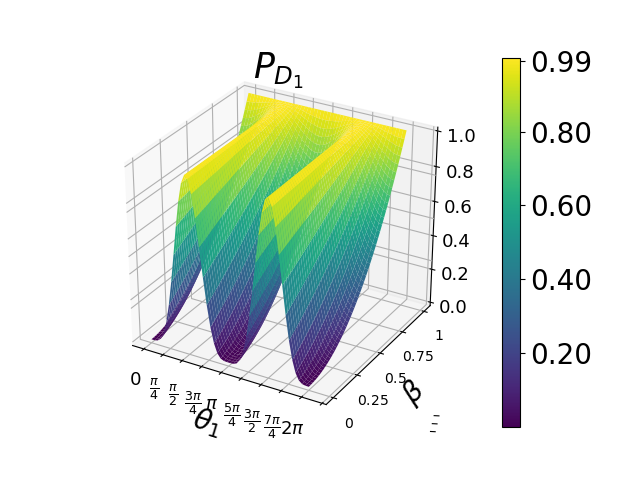
\includegraphics[width=\linewidth]{images/PD1_h.png}
\caption{$P_{1D_{1}}$}
\label{fig:BS1}
\end{subfigure}
\begin{subfigure}[b]{0.4\linewidth}
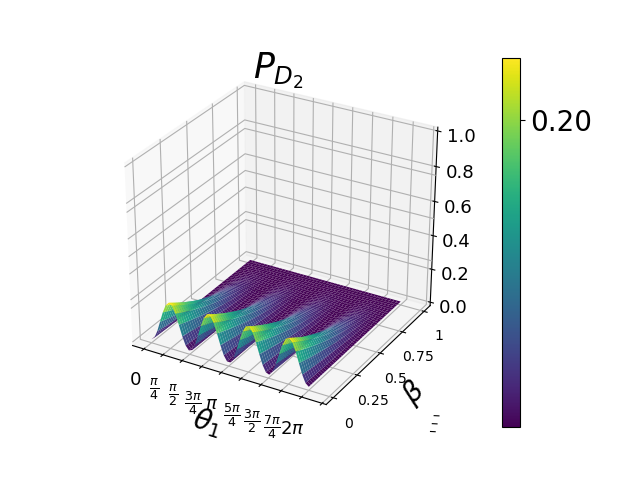
\includegraphics[width=\linewidth]{images/PD2_h.png}
\caption{$P_{1D_{2}}$}
\label{fig:westminster_aerea}
\end{subfigure}
\begin{subfigure}[b]{0.4\linewidth}
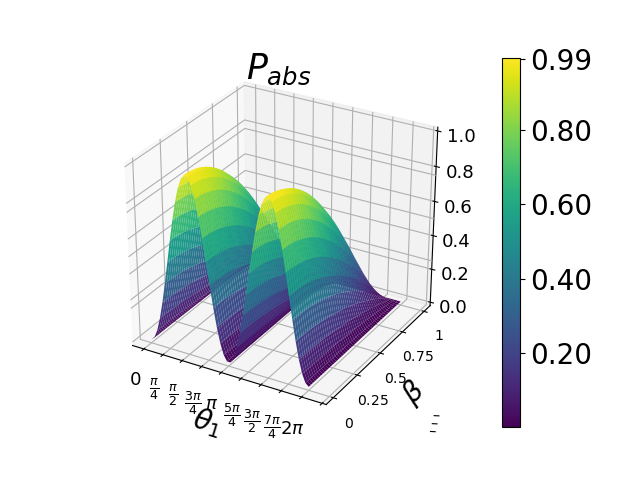
\includegraphics[width=\linewidth]{images/PAbs_v.png}
\caption{$P_{1abs}$}
\label{fig:BS1}
\end{subfigure}
\caption{Probability distributions of detection and absorption of the photon with the optical chopper placed in the horizontal path. In these plots $\theta_{2}=\frac{\pi}{2}-\theta_{1}$ and $\gamma_{2}-\gamma_{1}=0$, subfigure (a) corresponds to $P_{1D_{1}}$, (b) to $P_{1D_{2}}$ and (c) to $P_{1abs}$. When the sine is in the positive cycle (see Eqs. \ref{beta111}, \ref{beta11}, \ref{beta1})  the transmission coefficient is $\beta=1$ (there is no obstacle), otherwise we get the transmission coefficient is $\beta$ (the transmission coefficient of the material the chopper is made of) so the system alternates between the probabilities given by those values periodically.}
\label{P3chopper}
\end{figure}

where $\alpha$ is the absorption coefficient of the material part of the chopper. By using this notation we have the same case as in the previous section, except this time $f^2 \neq 1$ :

\begin{align}
|a|^2=a \alpha,\qquad |f_{material}|^2=f_{material} \beta,
\end{align}

which we can generalize to obtain:

\begin{equation}
|a|^n=a\alpha^{n-1},\qquad|f_{material}|^n=f_{material} \beta^{n-1}.
\end{equation}

In this form:

\begin{equation}
|f|^2=  \frac{\abs{\alpha}^2}{2} \mathrm{sgn}(\sin(wt)) +\frac{1+\abs{\beta}^2}{2}.
\end{equation}

\begin{figure}[t!]
\centering
\begin{subfigure}[b]{0.4\linewidth}
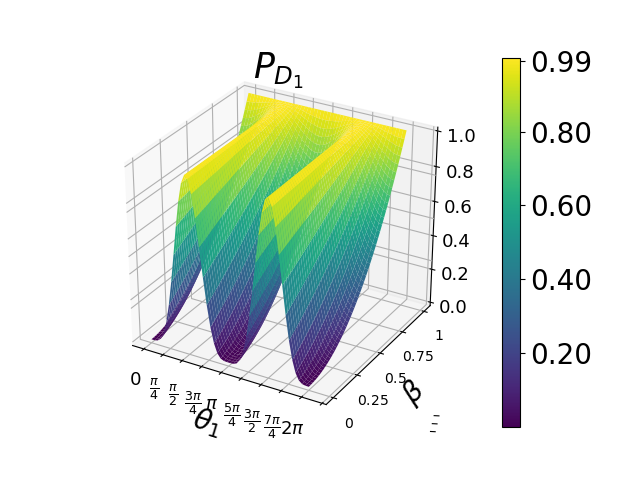
\includegraphics[width=\linewidth]{images/PD1_h.png}
\caption{$P_{2D_{1}}$}
\label{fig:BS1}
\end{subfigure}
\begin{subfigure}[b]{0.4\linewidth}
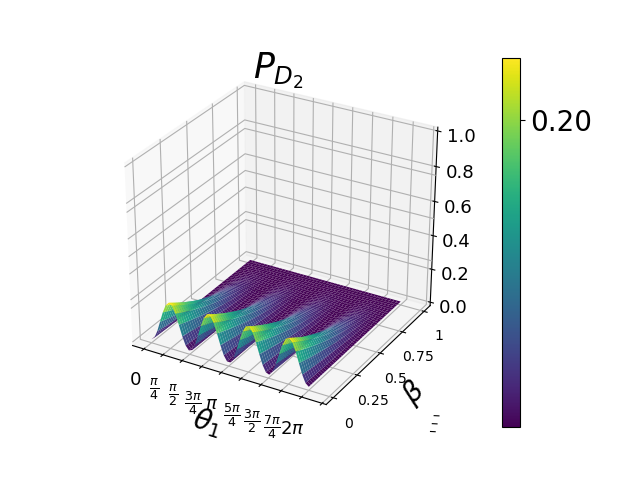
\includegraphics[width=\linewidth]{images/PD2_h.png}
\caption{$P_{2D_{2}}$}
\label{fig:westminster_aerea}
\end{subfigure}
\begin{subfigure}[b]{0.4\linewidth}
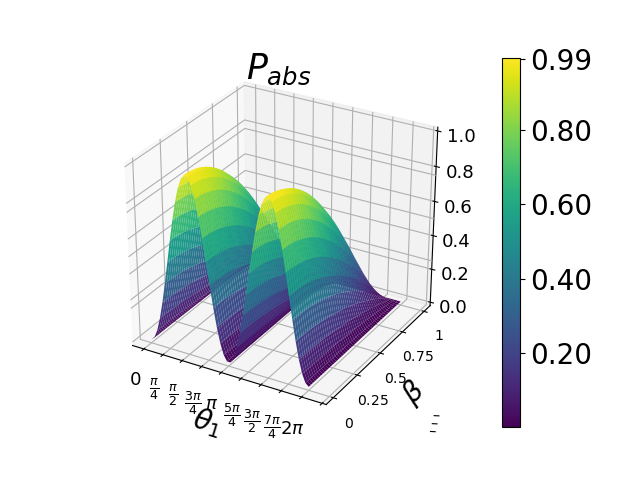
\includegraphics[width=\linewidth]{images/PAbs_v.png}
\caption{$P_{2abs}$}
\label{fig:BS1}
\end{subfigure}
\caption{Probability distributions of detection and absorption of the photon with the optical chopper placed in the horizontal path. In these plots $\theta_{2}=\frac{\pi}{2}-\theta_{1}$ and $\gamma_{2}-\gamma_{1}=0$, subfigure (a) corresponds to $P_{2D_{1}}$, (b) to $P_{2D_{2}}$ and (c) to $P_{2abs}$. When the sine is in the positive cycle (see Eqs. \ref{beta111}, \ref{beta11}, \ref{beta1}) the transmission coefficient is $\beta=1$ (there is no obstacle), otherwise we get the transmission coefficient is $\beta$ (the transmission coefficient of the material the chopper is made of) so the system alternates between the probabilities given by those values periodically.}
\label{P4chopper}
\end{figure}

Substituting these expressions in the results of the previous section yields the probability distributions shown in Fig. \ref{P3chopper}:


\begin{comment}
\begin{figure}[h]
\centering
\begin{subfigure}[b]{0.40\linewidth}
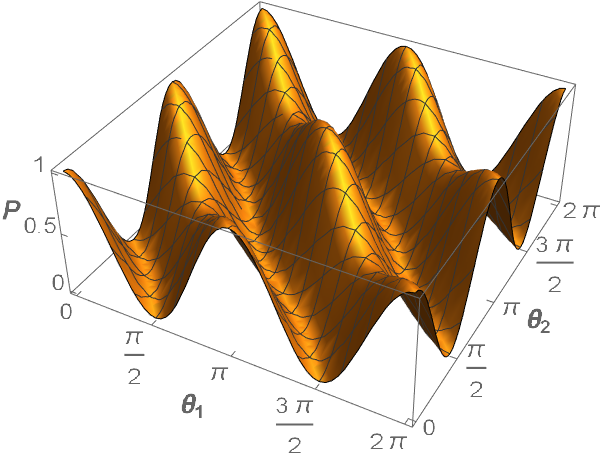
\includegraphics[width=\linewidth,height=2.5 cm]{images/pcd21.png}
\caption{$P_{1D_{2}}$ in the first cycle }
\label{fig:BS1}
\end{subfigure}
\begin{subfigure}[b]{0.40\linewidth}
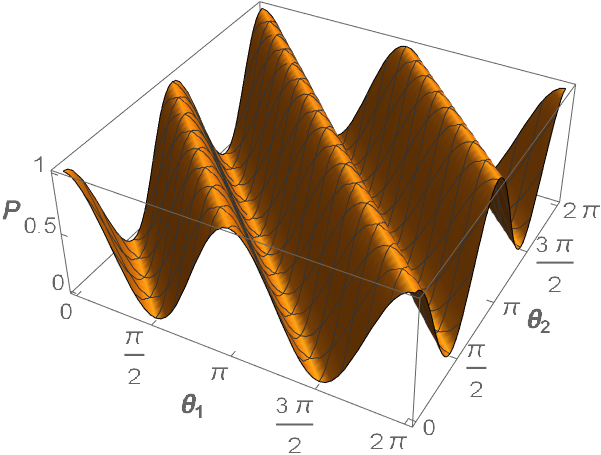
\includegraphics[width=\linewidth,height=2.5 cm]{images/pcd22.png}
\caption{$P_{1D_{2}}$ in the second cycle}
\label{fig:BS1}
\end{subfigure}
\begin{subfigure}[b]{0.40\linewidth}
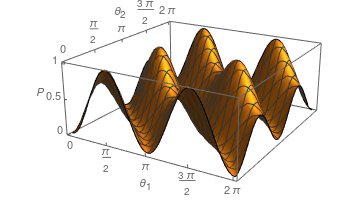
\includegraphics[width=\linewidth,height=2.5 cm]{images/pcd11.png}
\caption{$P_{1D_{1}} $ in the first cycle}
\label{fig:westminster_aerea}
\end{subfigure}
\begin{subfigure}[b]{0.40\linewidth}
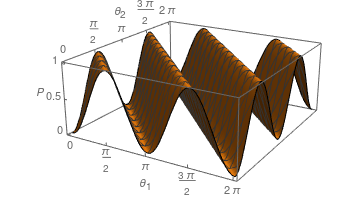
\includegraphics[width=\linewidth,height=2.5 cm]{images/pcd12.png}
\caption{$P_{1D_{1}} $ in the second cycle }
\label{fig:BS1}
\end{subfigure}
\begin{subfigure}[b]{0.40\linewidth}
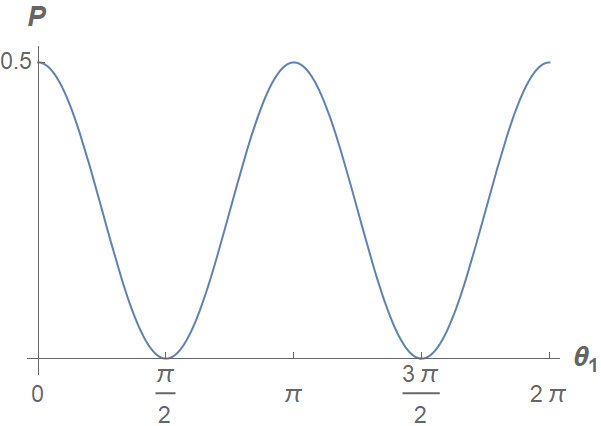
\includegraphics[width=\linewidth,height=2.5 cm]{images/PCABS.png}
\caption{$P_{1abs}$}
\label{fig:BS1}
\end{subfigure}
\caption{Probability distributions of detection and absorption of the photon with an optical chopper whose solid material is totally absorbent  placed in the horizontal path. In these plots  $\gamma_{2}-\gamma_{1}=0 $ and $\beta=0.5$, subfigure (a) corresponds to $P_{1D_{2}}$ in the second cycle, (b) to $P_{1D_{2}}$ in the first cycle, (c) and (d) to $P_{1D_{1}}$ in the second and first cycle, respectively, and (e) to $P_{1abs}$.}
\label{P3chopper}
\end{figure}
\end{comment}

\begin{align*}
P_{1D_{1}}=&\cos^2(\theta_{1})\sin^2(\theta_{2})\abs{f}^2+ \sin^2(\theta_{1})\cos^2(\theta_{2}) \label{sara1}\\
&+\frac{\Re{f} \sin(2\theta_{1})\sin(2\theta_{2})\cos(\gamma_{1}-\gamma_{2})}{2},\numberthis{}\\
P_{1D_{2}}=&\cos^2(\theta_{1})\cos^2(\theta_{2})\abs{f}^2+ \sin^2(\theta_{1})\sin^2(\theta_{2})\\
&-\frac{\Re{f} \sin(2\theta_{1})\sin(2\theta_{2})\cos(\gamma_{1}-\gamma_{2})}{2},\numberthis{}\\
P_{1abs}=&\abs{\alpha}^2 \cos^2(\theta_{1}), \label{sara2}\numberthis{}
\end{align*}

when the chopper is in the horizontal path. For the case that it is in the vertical one we obtain the following results. The probability distributions (\ref{sara1}-\ref{sara2}) and (\ref{sara3}-\ref{sara4})are shown in Fig. \ref{P3chopper} and \ref{P4chopper}:


\begin{comment}
\begin{figure}[!h]
\centering
\begin{subfigure}[b]{0.40\linewidth}
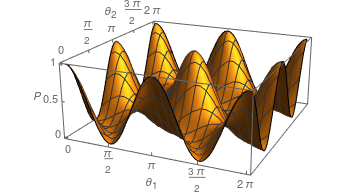
\includegraphics[width=\linewidth,height=2.5 cm]{images/p1cd21.png}
\caption{$P_{2D_{2}}$ in the first cycle }
\label{fig:BS1}
\end{subfigure}
\begin{subfigure}[b]{0.40\linewidth}
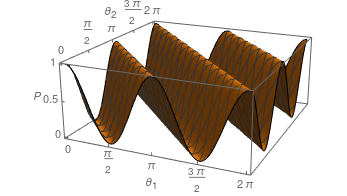
\includegraphics[width=\linewidth,height=2.5 cm]{images/p1cd22.png}
\caption{$P_{2D_{2}}$ in the second cycle}
\label{fig:BS1}
\end{subfigure}
\begin{subfigure}[b]{0.40\linewidth}
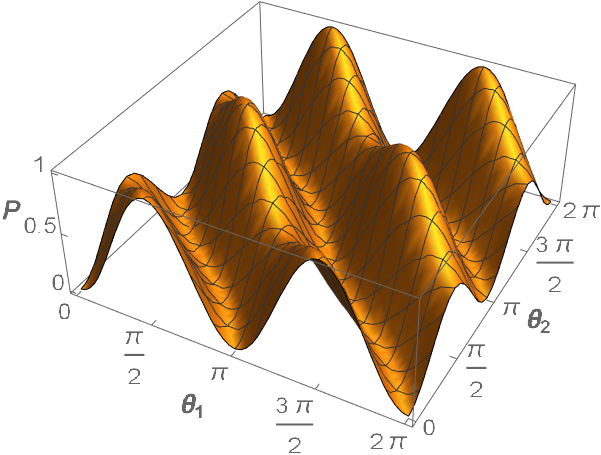
\includegraphics[width=\linewidth,height=2.5 cm]{images/p1cd11.png}
\caption{$P_{2D_{1}} $ in the first cycle}
\label{fig:westminster_aerea}
\end{subfigure}
\begin{subfigure}[b]{0.40\linewidth}
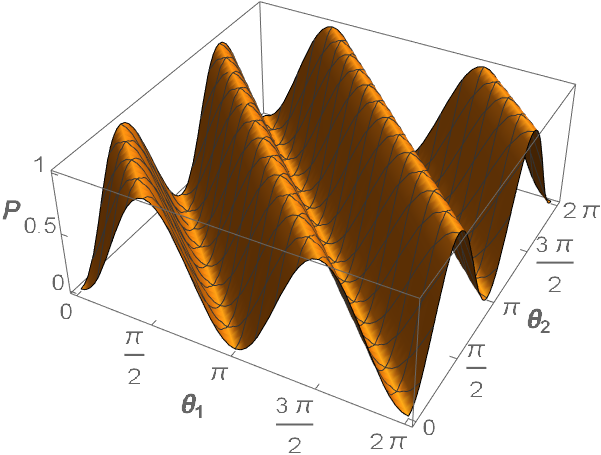
\includegraphics[width=\linewidth,height=2.5 cm]{images/p1cd12.png}
\caption{$P_{2D_{1}} $ in the second cycle }
\label{fig:BS1}
\end{subfigure}
\begin{subfigure}[b]{0.40\linewidth}
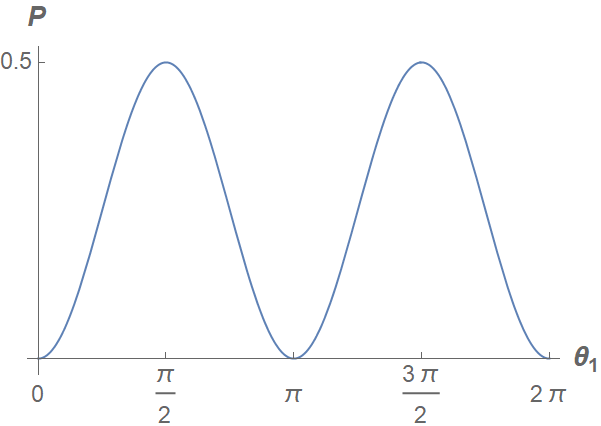
\includegraphics[width=\linewidth,height=2.5 cm]{images/PCABS2.png}
\caption{$P_{2abs}$}
\label{fig:BS1}
\end{subfigure}
\caption{Probability distributions of detection and absorption of the photon with an optical chopper whose solid material is totally absorbent  placed in the vertical path. In these plots  $\gamma_{2}-\gamma_{1}=0 $ and $\beta=0.5$, subfigure (a) corresponds to $P_{2D_{2}}$ in the second cycle, (b) to $P_{2D_{2}}$ in the first cycle, (c) and (d) to $P_{2D_{1}}$ in the second and first cycle, respectively, and (e) to $P_{2abs}$.}
\label{P4chopper}
\end{figure}
\end{comment}
\begin{align*}
P_{2D_{1}}=&\cos^2(\theta_{1})\sin^2(\theta_{2})+\abs{f}^2 \sin^2(\theta_{1})\cos^2(\theta_{2})\label{sara3}\\
&+\frac{\Re{f} \sin(2\theta_{1})\sin(2\theta_{2})\cos(\gamma_{1}-\gamma_{2})}{2},\numberthis{}\\
P_{2D_{2}}=&\cos^2(\theta_{1})\cos^2(\theta_{2})+ \abs{f}^2 \sin^2(\theta_{1})\sin^2(\theta_{2})\\
&-\frac{\Re{f} \sin(2\theta_{1})\sin(2\theta_{2})\cos(\gamma_{1}-\gamma_{2})}{2},\numberthis{}\\
P_{2abs}=&\abs{\alpha}^2 \sin^2(\theta_{1}).\label{sara4}\numberthis{}
\end{align*}


As seen in this section, an optical chopper can be modeled as a device producing a square wave signal. As the time evolution of the system in this model is piecewise and periodic the probability distribution of the system will be oscillating between the probability distribution of a semitransparent object ($0<\beta<1$) and that of a transparent object ($\beta=1$).

\pagebreak

\chapter{High-efficiency  Mach-Zehnder interferometer  }

In the previous section, we discussed a technique to confirm the presence of an object without interacting with it. In that procedure, we demonstrate that we can verify the presence of the object with a maximum probability of $\frac{1}{2}$ for the Elitzur-Vaidman case.


In this section, we will explore the possibility of improving that probability by considering a nested Mach-Zehnder interferometer, which is an interferometer whose outputs go into subsequent beam splitters. Our proposal is inspired by the experiments discussed by Kwait et al \cite{5} and Azuma \cite{Azuma}. In their works, the authors state that the probability of interaction-free measurements can be arbitrarily close to one when considering a series of connected interferometers, each one with an absorbent or semitransparent object, see Fig. \ref{Nmach}. The presence of an object in the upper path of each interferometer can be thought of as a series of measurements addressed to determine which path (upper or lower) the photon is traveling in. These interrogations will inhibit the transference from the lower (incident) path to the upper one, thus increasing the probability that the photon is detected in the lower path detector $D_{1}$ in a kind of discrete Zeno effect \cite{5}.

  We will place an identical semitransparent object in the upper path of our nested interferometer after each beam splitter except for the last one. Our signal photon will enter the interferometer through the lower path, as shown in Fig. \ref{Nmach}. We have $N$ beam splitters and $N-1$ absorbers before the output. To be consistent with the existing literature and in order to compare our result with those previously reported results we will use the same notation as Kwait et al. \cite{5}.
 
 
Instead of using the Horizontal-Vertical basis, we will use a path $a$ -path $b$ basis. That is an ``up-down" basis. We will say that the photon is in the state $\ket{1}$ if it is in path $a$ and in the state $\ket{2}$ if it is in path $b$. The main advantage of using this basis is that the mirror matrices are proportional to the identity because they keep the photon on the same path.
 
\begin{comment}
 In order to use the same beam splitter matrix as before and be consistent with the literature \cite{5}, we choose the reflectivity of the $N$ $BS$ to be modeled by $cos(\theta)$ instead of $i\sin(\theta)$, as a consequence the transmissivity is now $i\sin(\theta)$. 
 \end{comment}
 
 
  We will model the imperfect absorber using a non-unitary diagonal matrix just as was done by  Azuma \cite{Azuma}. Azuma used a matrix of the form:
 
 \begin{equation}
 A_{Azuma}=\begin{pmatrix} \sqrt{n} & 0\\0& 1\end{pmatrix},
\label{absorber}
 \end{equation}
 
 where the transmissivity $\beta$  is such that $|\beta|^{2}=n$. In our case, each imperfect absorber is a $BS$. We will then consider that each of the $N$ $BS$ has a reflectivity $\cos(\theta)$ and a transmitivity $i\sin(\theta)$. Thus, in our model, the imperfect absorbers are modeled by the matrix
 

\begin{equation}
 A_{BS}=\begin{pmatrix} \sin(\theta) & 0\\0& 1\end{pmatrix}.
\label{absorber1}
\end{equation}

\begin{figure}[t!]
\centering
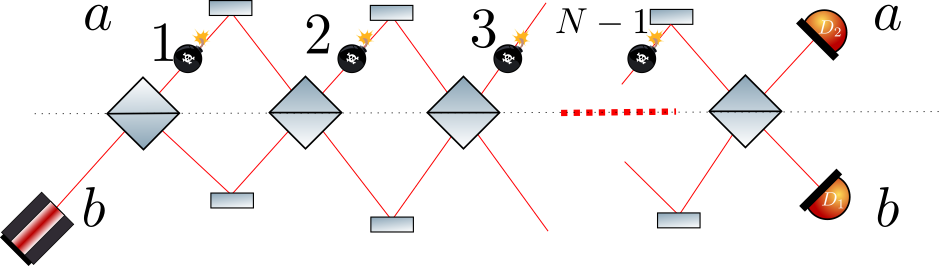
\includegraphics[width=\linewidth]{images/nmach2.png}
\caption{Nested Mach-Zehnder interferometer  with identical imperfect absorbers.}
\label{Nmach}
\end{figure}


We consider that the photon is incident through the path $b$. Thus the initial state of the system is $\ket{2}$. The final state can be obtained by applying the operators corresponding to each of the optical elements involved to the initial state $\ket{2}$. We consider both mirrors to be identical so that the phase they induce ends up being a global phase which does not affect the probabilities. First, we study the case with no obstacles in any of the arms of the interferometer. The evolution of the initial state $\ket{2}$ can be calculated by applying on it the matrix of each $BS$, but notice that the multiplication of two $BS$ matrices is

\begin{align*}
BS_{i+1} \cdot BS_{i}&=\begin{pmatrix} \cos(\theta_{i+1}) & i \sin(\theta_{i+1}) \\ i \sin(\theta_{i+1}) & \cos(\theta_{i+1}) \end{pmatrix}  
\begin{pmatrix} \cos(\theta_{i}) & i \sin(\theta_{i}) \\ i \sin(\theta_{i}) & \cos(\theta_{i}) \end{pmatrix},\\
&=\begin{pmatrix} \cos(\theta_{i}+\theta_{i+1}) & i \sin(\theta_{i}+\theta_{i+1}) \\ i \sin(\theta_{i}+\theta_{i+1}) & \cos(\theta_{i}+\theta_{i+1}) \end{pmatrix}. \numberthis
\end{align*}


\section{Case of identical beam splitters when $\sum_{i=1}^{N}\theta_{i}=\frac{\pi}{2}$}

Assuming that the interferometer contains $N$ identical beam splitters, then the nested action of all of them can be represented by $N$ $BS$ that are identical and sum to $\frac{\pi}{2}$:

\begin{equation}
BS^{N}=\begin{pmatrix} \cos(N\Theta) & i \sin(N\Theta) \\ i \sin(N\Theta) & \cos(N\Theta) \end{pmatrix},
\end{equation}

where $\Theta=\theta_{i}$. As an important particular case, we can ask  $\Theta=\frac{\pi}{2N}$, so they sum up to $\frac{\pi}{2}$ our restriction from chapter 3, so we have:

\begin{equation}
BS^{N}=\begin{pmatrix} 0 & i  \\ i  & 0 \end{pmatrix}.
\end{equation}

If all the mentioned conditions are satisfied, we will always detect the photon in the path b detector $D_{1}$.

 \begin{figure}[t]
\centering
\begin{subfigure}[b]{0.45\linewidth}
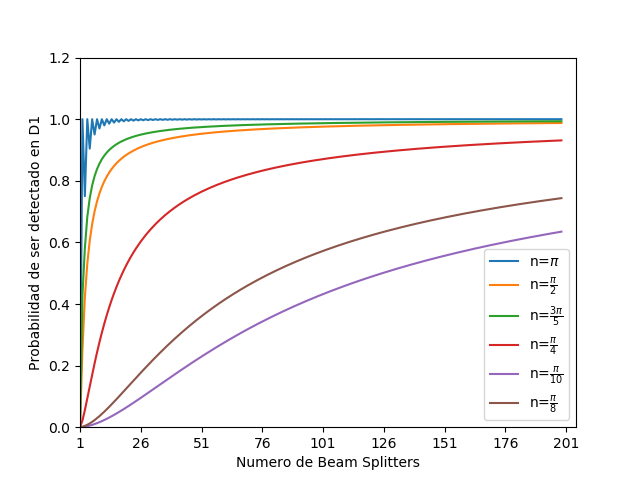
\includegraphics[width=\linewidth,height=5 cm]{images/BS_Azuna.png}
\caption{$P_{D_{1}}$}
\label{fig:BS1}
\end{subfigure}
\begin{subfigure}[b]{0.45\linewidth}
\includegraphics[width=\linewidth,height=5 cm]{images/BS_AzunaD2.png}
\caption{$P_{D_{2}}$}
\label{fig:westminster_aerea}
\end{subfigure}
\begin{subfigure}[b]{0.45\linewidth}
\includegraphics[width=\linewidth,height=5 cm]{images/absorbido_azuna.png}
\caption{$P_{abs}$}
\label{fig:BS1}
\end{subfigure}
\caption{Detection probabilities the nested interferometer with $\Theta=\frac{\pi}{2N}$ and the values of $\theta$ indicated in each plot, the detection probability in $P_{D_{1}}$ (a), $P_{D_{2}}$ (b) or that the photon is ``absorbed'' $P_{abs}$ (c). }
\label{Azuma1}
\end{figure}

  Let us see what happens, for this particular value of $\Theta$ when we introduce imperfect absorbers, see Fig. \ref{Nmach}, all of them with the same optical properties. The incident photon interacts with the first beam splitter and its state is transformed into a linear superposition of the state representing the photon in path $a$ and the state representing the photon in path $b$. The photon in path $b$ state interacts with the first imperfect absorber, and then its state is recombined in the second beam splitter. This process is repeated until the photon state has crossed through the $N$ beam splitters. We can write the whole process as 


\begin{equation}\ket{2}\xrightarrow[\text{interferometers}]{\text{Nested}}(B \cdot A)^{N-1}B \ket{2}.
\end{equation}

The detection probabilities are given by:

\begin{align}
&P_{D_{1}}=|\bra{2} (B \cdot A)^{N-1}B \ket{2}|^2,\label{comenta}\\
&P_{D_{2}}=|\bra{1} (B \cdot A)^{N-1}B \ket{2}|^2,\\
&P_{abs}=1-P_{D_{1}}-P_{D_{2}}.
\label{comentatio}
\end{align}
 
 
To obtain said probabilities, as well as the behavior of the system for varying $N$, we used a computer. The program was written in python and yielded the results shown in Fig. \ref{Azuma1}




Fig. \ref{Azuma1} shows  different probabilities as we increase $N$. A program in python was used to evaluate the values of the probabilities \ref{comenta}-\ref{comentatio} for diverse values of $N$ and $\theta$. We can see that the probability of detection in $D_{1}$ resembles the results reported by Azuma \cite{Azuma}. Moreover, if we want to perform the experiment varying continuously the transitivity of the obstacle, we can use a polarizer and analyzer \cite{nosirve}.  This case is described by the same mathematics as that of beam splitters \cite{nosirve}. Unlike other absorbers, this can be manipulated continually, giving us a way to test these curves experimentally. 



 \section{Case of identical beam splitters $\theta_{i}=\theta$}
 
In the previous section, we consider $N$-dependent $\theta$, $\Theta = \frac{\pi}{2N}$. One may wonder how the system behaves for growing $N$ but fixed $\theta$, a natural question is if this allows us to improve the detection probability $P_{D_{1}}$. The results can be obtained considering the expressions \ref{comenta}-\ref{comentatio} with the the $BS$ matrix \ref{BS_matrix}. The corresponding probabilities are shown in Fig. \ref{Azuma2}. We can see that even though $P_{D_{1}}$ grows for small values of $N$ it decreases and approaches zero very quickly as the value of $N$ increases. Correspondingly, one may observe that the absorption probability $P_{abs}$ rapidly approaches one. We conclude that this device is not efficient if the aim is to maximize the detection probability $P_{D_{1}}$. However, in a situation where the absorption probability needs to be improved this scheme would prove useful.

\begin{figure}[!t]
\centering
\begin{subfigure}[b]{0.45\linewidth}
\includegraphics[width=\linewidth]{images/BsFijo_azumaD1.png}
\caption{$P_{D_{1}}$}
\label{fig:BS1}
\end{subfigure}
\begin{subfigure}[b]{0.45\linewidth}
\includegraphics[width=\linewidth]{images/BsFijo_azumaD2.png}
\caption{$P_{D_{2}}$}
\label{fig:westminster_aerea}
\end{subfigure}
\begin{subfigure}[b]{0.45\linewidth}
\includegraphics[width=\linewidth]{images/BsFijo_azumaabs.png}
\caption{$P_{abs}$}
\label{fig:BS1}
\end{subfigure}
\caption{Detection probabilities as functions of $N$ with 50:50 as semitransparent objects in each interferometer, $P_{D_{1}}$(a), $P_{D_{2}}$(b) and the probability of photon absorption (c).}
\label{Azuma2}
\end{figure}




 


\section{Case $\theta_{i} \neq \theta_{j}$ and $\sum_{i=1}^{N}\theta_{i}=\frac{\pi}{2}$}

As we explored at the beginning of this chapter, what gives us distinguishability between the case where we have an object in one of the arms of the interferometer and when there is no obstacle, is the fact that when the sum of the angles $\theta_{i}$ is $\frac{ \pi}{2}$.


Now, the question is if we could obtain similar results if we use different angles $\theta_{i}$ that sum up to $\frac{\pi}{2}$? The answer is positive. To illustrate this fact let us recall that the probability of detection in $D_{1}$ is given by Eq. \ref{comentatio}

\begin{equation*}
P_{D_{1}}=|\bra{2} (BS \cdot A)^{N-1}BS \ket{2}|^2.
\end{equation*}

Let us fix $N$, as, e.g. $N=3$. Thus $P_{D_{1}}$ is given by:
\small
\begin{align*}
&P_{D_{1}}=\beta^{4} \sin^{2}{\left(\theta_{1} \right)} \sin^{2}{\left(\theta_{3} \right)} \cos^{2}{\left(\theta_{2} \right)} + 2 \beta^{3} \sin{\left(\theta_{1} \right)} \sin{\left(\theta_{2} \right)} \sin{\left(\theta_{3} \right)} \sin{\left(\theta_{1} + \theta_{3} \right)} \cos{\left(\theta \right)} \cos{\left(\theta_{2} \right)} \\
 & - 2 \beta^{2} \sin{\left(\theta_{1} \right)} \sin{\left(\theta_{3} \right)} \cos{\left(2 \theta \right)} \cos{\left(\theta_{1} \right)} \cos^{2}{\left(\theta_{2} \right)} \cos{\left(\theta_{3} \right)} + \beta^{2} \sin^{2}{\left(\theta_{2} \right)} \sin^{2}{\left(\theta_{1} + \theta_{3} \right)} \\
 & - 2 \beta \sin{\left(\theta_{2} \right)} \sin{\left(\theta_{1} + \theta_{3} \right)} \cos{\left(\theta \right)} \cos{\left(\theta_{1} \right)} \cos{\left(\theta_{2} \right)} \cos{\left(\theta_{3} \right)} + \cos^{2}{\left(\theta_{1} \right)} \cos^{2}{\left(\theta_{2} \right)} \cos^{2}{\left(\theta_{3} \right)},
\end{align*}
\normalsize

where $\beta$ is the transparency of the object and $\theta$ the phase it induces. Now let us see what happens in the case we expect the maximum absorption ($\beta=0$): 

\begin{equation}
P_{D_{1}}=\cos^{2}{\left(\theta_{1} \right)} \cos^{2}{\left(\theta_{2} \right)} \cos^{2}{\left(\theta_{3} \right)}.
\end{equation}

If we make $\theta_{i}=\frac{\pi}{2N}$, $i=1, 2, 3$ just like in section 6.1 we obtain

\begin{equation}
P_{D_{1}}=\cos^{6}{\left(\frac{\pi}{6} \right)}=\frac{27}{64}=0.421875.
\end{equation} 

If instead, we preserve that the sum is $\frac{\pi}{2}$,  but we use different angles $\theta_{1}$ for instance, $\theta_{1}=\frac{\pi}{4}$, $\theta_{2}=\frac{\pi}{6}$ and $\theta_{3}=\frac{\pi}{12}$, then we get 

\begin{equation}
P_{D_{1}}=\cos^{2}{\left(\frac{\pi}{4} \right)} \cos^{2}{\left(\frac{\pi}{6} \right)} \cos^{2}{\left(\frac{\pi}{12} \right)}=0.3499.
\end{equation}

Similar results are expected for higher values of $N$. As Kwait et al \cite{exp} argued, if the photon is to be detected in either $D_{1}$ or $D_{2}$ then it always was reflected back to path $b$ so it did not interact with the object. The probability $P_{D_{1}}$ will be the product of the square of the cosines of $\theta_{i}$, $i=1,2,3,\dots,N$. Our results are in agreement with those reported in reference \cite{exp} for $\beta=0$, if instead, we use semitransparent objects then the probabilty of detection $P_{D_{1}}$ is reduced (see figure \ref{reducidito})

\begin{figure}[!t]
\begin{subfigure}[b]{0.4\linewidth}
\includegraphics[width=\linewidth]{images/beta_theta2.png}
\caption{$\beta=0$}
\label{fig:BS1}
\end{subfigure}
\begin{subfigure}[b]{0.4\linewidth}
\includegraphics[width=\linewidth]{images/beta_theta.png}
\caption{$\beta=0.5$}
\label{fig:westminster_aerea}
\end{subfigure}

\caption{Behaviour of the probability when we use different angles for $N=3$ such that their sum is $\frac{\pi}{2}$, we used $\beta$=0 for (a) and $\beta$=0.5 for (b).}
\label{recidito}
\end{figure}

From this analysis, we can conclude that the best bomb detector we could build would be one whose bomb is perfectly absorbent in an array of $N$ interferometers such that the beam splitters have a reflectance given by $\theta_{i}=\Theta=\frac{\pi}{2 N}$, $i=1,2,\dots,N$. However, in practice, such an object is difficult to realize and that is why models with semitransparent objects are useful.
 

\section{Does the phase matter?}

As we saw in the previous section, if we use nested interferometers we can increase the probability of detection in $D_{1}$ arbitrarily close to unity, by placing semitransparent objects in the path $a$ of the array (see figure \ref{Nmach}). However, neither in the treatment by Azuma \cite{Azuma} nor in our previous models the phase the object induces was considered. Is it unimportant?

To answer this question we explore how the object inducing a phase would affect our previous calculations. To introduce that phase, one simply modifies Eqs. \ref{absorber} or \ref{absorber1}. by expresing $\beta$ in its polar representation, this is equivalent to considering a phase shifter in the same path of the object. The resulting matrix is:

\begin{equation}
 A=\begin{pmatrix} |\beta| e^{i \theta}& 0\\0&  1\end{pmatrix}.
 \end{equation}

Following the same procedure as in section 6.1, we obtain the probabilities $P_{D_{1}}$, $P_{D_{2}}$, $P_{abs}$ given by the expressions \ref{comenta}-\ref{comentatio} with the change $|\beta|\xrightarrow{}|\beta|e^{i\theta}$.

\begin{figure}[!t]
\centering
\begin{subfigure}[b]{0.30\linewidth}
\includegraphics[width=\linewidth]{images/Azuma_phases2.png}
\caption{$N=2$}
\end{subfigure}
\begin{subfigure}[b]{0.30\linewidth}
\includegraphics[width=\linewidth]{images/Azuma_phases5.png}
\caption{$N=5$ }
\label{fig:BS1}
\end{subfigure}
\begin{subfigure}[b]{0.30\linewidth}
\includegraphics[width=\linewidth]{images/Azuma_phases10.png}
\caption{$N=10$ }
\label{fig:BS1}
\end{subfigure}
\begin{subfigure}[b]{0.30\linewidth}
\includegraphics[width=\linewidth]{images/Azuma_phases100.png}
\caption{$N=100$}
\label{100}
\end{subfigure}
\begin{subfigure}[b]{0.30\linewidth}
\includegraphics[width=\linewidth]{images/Azuma_phases1000.png}
\caption{$N=1000$ }
\label{1000}
\end{subfigure}
\caption{Behaviour of probabilities as $N$ grows and we vary $\theta$ for $\beta=0.5$, (a) $N$=2, (b) $N$=5, (c) $N$=10, (d) $N$=100, (e) $N$=1000.}
\label{con_fase}
\end{figure}

As we see from Fig. \ref{con_fase} the phase is important when $N$ is small (Figs. \ref{con_fase} (a-c)). As $N$  grows the variations due to the phase $\theta$ become smaller Fig. \ref{con_fase} (d) until the probability becomes constant in $\theta$ Fig \ref{con_fase} (e) when $N$ is too large.

These plots, allow us to determine the values of the phases that would improve our bomb detector for unbalanced interferometers (interferometers with misalignments), such as the one developed in \cite{Chao_2018} for given values of $|\beta|$ and $N$.

\section[Optical choppers case]{Optical chopper as imperfect absorbers in  an array of $N$ interferometers}

In this next section, we will replace the $N-1$ imperfect absorbers by $N-1$ synchronized identical optical choppers. To model an optical chopper the following matrix could be used:
 \begin{figure}[!t]
 
\centering
\begin{subfigure}[b]{0.45\linewidth}
\includegraphics[width=\linewidth]{images/ChopperD1.png}
\caption{$P_{D_{1}}$}
\label{fig:BS1}
\end{subfigure}
\begin{subfigure}[b]{0.45\linewidth}
\includegraphics[width=\linewidth]{images/ChopperD2.png}
\caption{$P_{D_{2}}$}
\label{fig:westminster_aerea}
\end{subfigure}
\begin{subfigure}[b]{0.45\linewidth}
\includegraphics[width=\linewidth]{images/Chopper_abs.png}
\caption{$P_{abs}$}
\label{fig:BS1}
\end{subfigure}
\caption{Behavior of the detection probabilities as functions of $N$ for an array of $N$ interferometers with optical choppers as imperfect absorbers. Plot (a) shows the probability of detection in $D_{1}$, (b) the probability of detection in $D_{2}$ and (c) the probability that the photon is absorbed.}
\label{fig:several_chpper}
\end{figure}

\begin{equation}
A_{chopper}=\begin{pmatrix} f & 0 \\ 0 & 1 \end{pmatrix},
\end{equation}

where

\begin{equation}
f=\left(\frac{1-\mathrm{sgn}(\sin(wt))}{2} \right)\beta+\frac{1+\mathrm{sgn}(\sin(wt))}{2}.
\end{equation}

As $f$ is a piecewise function matrix $A_{chopper}$ will alternate between two values of the transmitivity, namely, $\beta$ and 1.



In the positive semi cycle we have $f=1$, while on the negative one $f=\beta$. For convenience, we will rewrite the matrix in Eq. \ref{absorber} in terms of $|\beta|$. In this way, in the positive semi cycle, we will have the case of the nested interferometer with no object which is the same as having $\beta=1$. In turn, in the negative semi cycle, we will recover  Azuma's case.



 

Fig. \ref{fig:several_chpper} shows the probability distributions for optical choppers with different transparencies. The blue line represents a ``gap" in the chopper, and the other lines represent the ``material" parts.
\section{Towards Wheeler's gedanken experiment}

One of the main reasons why the Mach-Zehnder interferometer is so popular is that it allows us to study fundamental facts about quantum theory such as Bohr's complementary principle. This is well explained in the reference \cite{delayed}. In this article, the authors wonder if a photon behaves like a particle or a wave in a Mach-Zehnder interferometer. The idea is better explained with the following the gedanken experiment proposed by Wheeler \cite{delayed}.


\begin{figure}[t!]
\begin{subfigure}{0.45\linewidth}
  \centering
  % include first image
\includegraphics[width=\linewidth]{images/wheeler1.png}
\caption{}
\label{wheeler1}
\end{subfigure}
\begin{subfigure}{0.45\linewidth}
  \centering
  % include second image
\includegraphics[width=\linewidth]{images/wheeler2.png}
\caption{}
\label{wheeler2}
\end{subfigure}
\begin{subfigure}{0.45\linewidth}
  \centering
  % include second image
\includegraphics[width=\linewidth]{images/wheeler3.png}
\caption{}
\label{wheeler3}
\end{subfigure}
\caption{Subfigure (a) shows a Mach-Zehnder interferometer with both $BS$ being 50:50. The detection always occurs at $D_{1}$. Subfigure (b) shows a Mach-Zehnder interferometer without the second $BS$ and subfigure (c) shows a Mach-Zehnder interferometer with the second $BS$ is a in a superposition of being present and absent.}
\label{Wheeler}
\end{figure}

Let us picture a Mach-Zehnder interferometer like the one shown in Fig. \ref{Wheeler} (a), with both $BS$ being 50:50 beam splitters. Now, imagine that we pump a single photon into the interferometer through the horizontal input port. From the analysis of section 3.2 we get (see Eq. \ref{pp_wheler}).

\begin{equation}
P_{D_{1}}=\frac{1+\cos(\gamma_{2}-\gamma_{1})}{2}, \qquad P_{D_{2}}=\frac{1-\cos(\gamma_{2}-\gamma_{1})}{2}. \label{pp_wheler}
\end{equation}

 If the difference in the optical path is $\gamma_{1}-\gamma_{2}=0$  we obtain certainty that where the detection will occur in $D_{1}$. Yet, we have no information on which path the photon took.



Now, let us consider the new arrangement in which the second beam splitter has been removed (Fig. \ref{Wheeler} (b)). It is clear that in this case, we will have no certainty in which detector ($D_{1}$ or $D_{2}$) the photon will be detected, as it has an equal probability of being detected in $D_{1}$ or $D_{2}$. However, once the photon is detected, we have complete information on which path the photon took.

\begin{figure}[t!]
\centering
\begin{subfigure}[b]{0.40\linewidth}
\includegraphics[width=\linewidth]{images/pd1_2.png}
\caption{$P_{D_{1}}$}
\end{subfigure}
\begin{subfigure}[b]{0.40\linewidth}
\includegraphics[width=\linewidth]{images/pd2_2.png}
\caption{$P_{D_{2}}$ }
\label{fig:BS1}
\end{subfigure}
\begin{subfigure}[b]{0.40\linewidth}
\includegraphics[width=\linewidth]{images/pabs_2.png}
\caption{$P_{D_{2}}$ }
\label{fig:BS1}
\end{subfigure}
\caption{Continuos transition between wave and particle behaviour with 50:50 $BSs$. (a) shows the probability that the photon is detected at $D_{1}$, (b) at $D_{2}$ and (c) the probability  that the photon is absorbed by the object.}
\label{transzuri}
\end{figure}


In the first situation, we have wave-like behavior while in the second one a particle-like behavior. In the Wheeler Gedanken experiment, the idea is to have the second beam splitter in a superposition of being present and absent. It seems that, before entering the experiment, the photon somehow decides whether it is going to behave as a particle or as a wave. This seems to be in accordance with Bohr's complementary principle. This is precisely what quantum delayed-choice experiments seek to rule out \cite{Ma}: to conclude if the photon has particle or wave behavior or even if it is in a continuous transition between these two very different behaviors while the experiment is running.
\begin{figure}[t!]
\centering
\begin{subfigure}[b]{0.40\linewidth}
\includegraphics[width=\linewidth]{images/pd1_2_pi3.png}
\caption{$P_{D_{1}}$}
\end{subfigure}
\begin{subfigure}[b]{0.40\linewidth}
\includegraphics[width=\linewidth]{images/pd2_2_pi3.png}
\caption{$P_{D_{2}}$ }
\label{fig:BS1}
\end{subfigure}
\caption{Continuous transition between wave and particle behavior with 25:75 BSs. The probability of detection in $D_{1}$ (a) and $D_{2}$ in (b)}
\label{pi/3}
\end{figure}

It was recently demonstrated \cite{Peruzzo, Kaiser2012} that there is a smooth transition between particle and wave behaviors. In those references, the authors implemented the Wheeler gedanken experiment using ``quantum'' $BS$, which is nothing but a $BS$ that is in a superposition state of being there and not being there (see Fig. \ref{Wheeler} (c)). They achieved this superposition through a controlled Hadarmard gate \footnote{As was discussed in the beam splitter section a Hadamard gate is equivalent to a 50:50 beam splitter}, acting as an identity gate if a control qubit is in the $\ket{0}$ state and as a Hadamard gate if the control qubit is in the state $\ket{1}$.  If the control qubit is in a superposition state, so will be the controlled Hadamard gate.




A similar situation arises in the interaction-free measurements, as taking a path means interaction with the object, and taking the other one means no interaction. The first $BS$ prepares the photon in a superposition state of taking both paths (note that this approach differs significantly from the one taken in \cite{Peruzzo,Kaiser2012} because our $BS$ differ from a Hadamard gate by more than a phase). Then both paths are recombined in the second $BS$ (recall we always have the second beam splitter on as in the experiments recently proposed \cite{Polino}).


If, we have both $BS$ in the setup, how can the transition between particle and wave behavior be achieved? The answer is simple, the object introduces two new parameters that can be tuned to change the behavior of the photon from particle to wave, since these properties change the probabilities at the output as was studied in previous sections. This was studied by Blanco-Garcia and  Rosas-Ortiz in \cite{azuri} for the 50:50 $BS$ case. Their results are in perfect agreement with the experiments performed by Peruzzo \cite{Peruzzo} and Kaiser \cite{Kaiser2012}. However, no experimental realization has been done to verify the model. Fig. \ref{transzuri} shows the transition from particle to wave behavior in the 50:50 case. (To make it more comparable to experiments we included the effect of misalignment $\gamma_{1},\gamma_{2}$, using $\Delta=\theta-\gamma_{1}-\gamma_{2}$, where $\theta$ is the phase induced by the object):


\begin{figure}[t!]
\centering
\begin{subfigure}[b]{0.3\linewidth}
\includegraphics[width=\linewidth]{images/pd1_3_pi4.png}
\caption{$P_{D_{1}}$}
\end{subfigure}
\begin{subfigure}[b]{0.3\linewidth}
\includegraphics[width=\linewidth]{images/pd2_3_pi4.png}
\caption{$P_{D_{2}}$ }
\label{fig:BS1}
\end{subfigure}
\begin{subfigure}[b]{0.3\linewidth}
\includegraphics[width=\linewidth]{images/pabs_3_pi4.png}
\caption{$P_{D_{2}}$ }
\label{fig:BS1}
\end{subfigure}
\begin{subfigure}[b]{0.3\linewidth}
\includegraphics[width=\linewidth]{images/pd1_5_pi4.png}
\caption{$P_{D_{1}}$ }
\label{fig:BS1}
\end{subfigure}
\begin{subfigure}[b]{0.3\linewidth}
\includegraphics[width=\linewidth]{images/pd2_5_pi4.png}
\caption{$P_{D_{2}}$ }
\label{fig:BS1}
\end{subfigure}
\begin{subfigure}[b]{0.3\linewidth}
\includegraphics[width=\linewidth]{images/pabs_5_pi4.png}
\caption{$P_{D_{2}}$ }
\label{fig:BS1}
\end{subfigure}
\caption{Continuous transition between wave and particle behaviour with 50:50 $BSs$ for $N=3$ and $N=5$. Plots in the top row correspond to $N=3$ and show the probability of detection at $D_{1}$ (a), $D_{2}$ (b) and the probability of the photon being ``lost''(c). Plots in the bottom row contain the corresponding probabilities for $N=5$,  $D_{1}$ (d),  $D_{2}$ (e)  ``absorbed'' (f).}
\label{varias}
\end{figure}

Fig. \ref{pi/3}, in turn, shows the result for 25:75 beam splitters. Observe that the behavior of the detection probability is preserved, this was expected as no matter the transmitivity of the beam splitter, if it takes the path where the object is and we have $\beta=0$ we know which path it took regardless of the phase, and as $beta$ increases start losing knowledge of the path the photon took and the phase starts to be important so that there can be interference. Alternatively, we could consider doing the same experiment using the constraint $\theta_{2}=\frac{\pi}{2}-\theta_{1}$ and just varying the magnitude of transparency of the object, and the values of the transparency of the beam splitters. We would obtain plots like \ref{P3chopper} and \ref{P4chopper} which exhibit a similar behavior where one can distinguish tell when the photon behaves like a particle, wave, or somewhere in between. This could be achieved by making variable beam splitters using polarized beam splitters \cite{variable}, with the same setup as in section 4.3 constraining ourselves to the values where $cos(\theta)$ is positive. Providing, yet another simple alternative to perform this kind of experiment.

\begin{figure}[t!]
\centering
\begin{subfigure}[b]{0.3\linewidth}
\includegraphics[width=\linewidth]{images/pd1_3.png}
\caption{$P_{D_{1}}$}
\end{subfigure}
\begin{subfigure}[b]{0.3\linewidth}
\includegraphics[width=\linewidth]{images/pd2_3.png}
\caption{$P_{D_{2}}$ }
\label{fig:BS1}
\end{subfigure}
\begin{subfigure}[b]{0.3\linewidth}
\includegraphics[width=\linewidth]{images/pabs_3.png}
\caption{$P_{D_{2}}$ }
\label{fig:BS1}
\end{subfigure}
\begin{subfigure}[b]{0.3\linewidth}
\includegraphics[width=\linewidth]{images/pd1_5.png}
\caption{$P_{D_{1}}$ }
\label{fig:BS1}
\end{subfigure}
\begin{subfigure}[b]{0.3\linewidth}
\includegraphics[width=\linewidth]{images/pd2_5.png}
\caption{$P_{D_{2}}$ }
\label{fig:BS1}
\end{subfigure}
\begin{subfigure}[b]{0.3\linewidth}
\includegraphics[width=\linewidth]{images/pabs_5.png}
\caption{$P_{D_{2}}$ }
\label{fig:BS1}
\end{subfigure}
\caption{Continuous transition between wave and particle behaviour with $\theta=\frac{\pi}{2N}$ $BS$s for $N=3$ and $N=5$. Plots in the top row correspond to $N=3$, they show the probability of detection at $D_{1}$ (a), $D_{2}$ (b) and the probability of the photon being ``lost''(c). Plotsin the bottom row correspond to $N=5$, they show the probability of detection at $D_{1}$ (d),  $D_{2}$ (e) and the probability of the photon being ``lost'' (f).}
\label{figvarias2}
\end{figure}

Fig. \ref{varias} shows the detection probabilities for a nested Mach-Zehnder interferometer of $N$ loops each one with a semitransparent object in one of its arms. In (a), (b) and (c) we can see the plots for $N=3$ while (d), (e) and (f) correspond to $N=5$. In these plots, we consider identical objects in each section of the interferometer. We also considered the beam splitters to be 50:50 and dropped the general form of the mirrors, selecting $\gamma_{1}=\gamma_{2}=\frac{\pi}{2}$). Note that we can see the transition between particle and wave behavior that happens for $\beta \approx 1$ which may suggest that the transition only happens for almost transparent or transparent objects. This is because the absorption probability tends to $1$ as $N$ grows, as we showed in section 6.2. 




We can circumvent this by using $BS$ with $\Theta=\frac{\pi}{2N}$, exploiting the quantum Zeno effect as mentioned in the previous section. The results are shown in Fig. \ref{figvarias2} for the same parameters used in Fig. \ref{varias}. Observe that the detection probability in $D_{1}$ is increased maintaining the transition oscillation between wave-like and particle-like behaviors.
                  



In conclusion, we proposed a simpler way to get the transition from wave and particle behavior, as \cite{Kaiser2012,Peruzzo} uses sophisticated equipment to implement a controlled Hadamard gate, we proposed a simpler scheme to achieve the same results both theoretically and experimentally. Besides requiring this complicated implementations a lot of debate has been arising since some claim that the experiments in \cite{Peruzzo,Kaiser2012}  can be explained with a two-dimensional classical variable \cite{Rossi,Chaves}, recently a proposal and implementation for an experiment that could not be explained in this way was presented in \cite{Polino}.
\pagebreak
\blankpage


\chapter{Experimental setup}


\section{Mach-Zehnder interferometer}

As we previously described in chapter 1, the Mach-Zehnder interferometer is made of two beam splitters ($BS_{1}$ and $BS_{2}$) and two mirrors ($M_{1}$ and $M_{2}$). We will use 50:50 beam splitters as in the Eliztur-Vaidman ``bomb detector'' (see Fig. \ref{newnewsingle}). To this end, we will use the following materials

\subsection{Materials}
\begin{itemize}
\item Two 50:50 beam splitters.
\item Two plane mirrors.
\item Two convergent lenses.
\item Two pinholes.
\item A red HeNe laser of 633nm wavelength.
\item High precision optomechanical instrumentation.
\end{itemize}

In order to obtain a good quality interference pattern, we aim to get the difference in optical paths to a minimum. According to the model presented in previous chapters, this is achieved if $|\gamma_{2}-\gamma_{1}|=2\pi n$. This alignment may be quite challenging in the laboratory. In order to accomplish this, we will consider the following approach for the alignment, as discussed in \cite{zuri}. To reduce $|\gamma_{2}-\gamma_{1}|$ as much as possible, the strategy is to align it by hand until a minimum is reached by tunning a micrometer screw attached to the mount of one of the mirrors.



\subsection{Setup and alignment of the interferometer}

In this section, we will describe in detail the procedure used to set up and align the Mach-Zehnder interferometer, up to get $|\gamma_{2}-\gamma_{1}|=2\pi n$, following the approach used in \cite{zuri}. It is necessary to be meticulous regarding the positions and characteristics of optical devices. For instance, it is necessary to consider that the $BS$ faces are not completely flat, and may change the propagation direction of the transmitted beam even when placed at $45\degree$ with respect to the incident beams. We will use 50:50 beam splitters

\begin{figure}[t!]
\centering
\includegraphics[scale=0.4]{images/mach_sara.png}
\caption{Experimental setup of the Mach-Zehnder interferometer.}
\label{newnewsingle}
\end{figure}

To align the interferometer two pinholes are needed to grant that the laser beam travels co-linear to the tapped holes of the optical table. One is placed as close as possible to the laser aperture, while the other one is placed near first beam splitter $BS_{1}$. In Fig.\ref{steps} (a-d) we show all the steps followed to align the interferometer.

\begin{figure}[t!]
\centering
\begin{subfigure}[b]{0.55\linewidth}
\includegraphics[width=8cm,height=4 cm]{images/first_step.png}
\caption{}
\label{fig:BS1}
\end{subfigure}
\begin{subfigure}[b]{0.55\linewidth}
\includegraphics[width=8cm,height=4 cm]{images/second_step.png}
\caption{}
\label{fig:BS1}
\end{subfigure}
\begin{subfigure}[b]{0.55\linewidth}
\includegraphics[width=8cm,height=4 cm]{images/third_step.png}
\caption{}
\label{fig:BS1}
\end{subfigure}
\begin{subfigure}[b]{0.55\linewidth}
\includegraphics[width=8cm,height=4 cm]{images/last_step.png}
\caption{}
\label{fig:westminster_aerea}
\end{subfigure}
\caption{Aligment of the Mach-Zehnder interferometer step by step, subfigure (a) shows the first step, (b) the second, (c) the third and (d) the fourth and last step.}
\label{steps}
\end{figure}



The first step is to place $BS_{1}$ at $45\degree$ with respect to the incoming beam so it does not introduce deviations in the transmitted beam. Thus, the reflected beam propagates at $90\degree$ with respect to the incident one. We use the pinholes to check that the output beams are colinear to the tapped holes of the table, so we know they are well aligned. Using two screens we may track the transmitted and reflected photons' paths, as shown in Fig. \ref{steps} (a).

The second step is to place the mirror $M_{2}$ in the path of the transmitted beam, the idea is to place $M_{2}$ in such a way that the reflected beam is colinear with the tapped holes of the optical table, in such a way that it is parallel to the reflected beam in $BS_{2}$. To do this, we first place the mirror in the desired and then check the alignment using a pinhole near $M_{2}$ and the other one near a second screen tracking the beam path as shown in Fig. \ref{steps} (b). In case it is necessary, we use the screws attached to the mirror's mount so that the beam goes through both pinholes.

In the third step, we dismount $M_{2}$ leaving its mount un site as it is already in the correct position. We place $M_{1}$, repeating step 2 in such a wat that the reflected beam is parallel to the transmitted beam in $BS_{1}$. The mirror $M_{1}$ is mounted on a sliding plate with a micro-metric screw in order to obtain more mobility that allows us to manipulate at will the difference in the path length of both arms of the interferometer. The expected result so far is shown in Fig. \ref{steps} (c). After completing this step we place $M_{2}$ once again.

The fourth and last step is to place $BS_{2}$ as it is shown in Fig. \ref{steps} (d). The reflected and transmitted beam should reach the marks recorded on the screens on steps two and three. As we are using a coherent light source we must be able to see the interference pattern at the screens by using convergent lenses to amplify the image generated at the output ports of the interferometer. Then by tunning the micrometer screw attached to the mount of $M_{1}$  we adjust the optical paths until we obtain the desired interference pattern. It is worthwhile to note that the smaller the length of the arms of the Mach-Zehnder interferometer, the better control over the length of the optical paths making the alignment easier.


\subsection{Varying optical paths}

To be able to see a good quality interference pattern, it is necessary to adjust the difference in optical paths $\delta \gamma$. The visibility of the interference fringes is a quantitative measure of the quality of the interference pattern. From the classical point of view, it is defined as \cite{hecht}:

\begin{equation}
V=\frac{I_{max}-I_{min}}{I_{max}+I_{min}},
\end{equation}

where $I_{max}$ is the maximum intensity and $I_{min}$ is the minimum intensity of the interference pattern. The ideal pattern has perfect visibility ($V$=1), which happens when $I_{min}=0$.

In quantum mechanics the intensity is proportional to the expected value of the photon number N \cite {glauber}, so that the visibility is given by:

\begin{equation}
V=\frac{N_{max}-N_{min}}{N_{max}+N_{min}},
\end{equation}

In an experiment, $N_{max}$ and $N_{min}$ correspond to the maximum and minimum coincidences counts, in the output ports, as we tune the micrometer screw.

Visibility counts will vary as we change the difference in optical paths $\delta\gamma$ by turning the micrometer screw attached to the mirror. The idea is to see how visibility changes with voltage and keep the maximum value that we can achieve to keep going with the rest of the experiments.

\section{Single-photon source}


In this chapter, we will describe the experimental setup considered to realize interaction-free measurements with semi-transparent objects. All the materials and results discussed in this and the next chapters are the outcome of experimental work that was developed under the facilities of the Quantum Phenomena Laboratory (QPL) at UPIITA, Instituto Politécnico Nacional. First, we will describe the setup and alignment of the Mach-Zehnder interferometer. Next, we will explain how to construct a single photon source using the SPDC process following the approach reported in \cite{maestria_procopio}. We will then recreate the Elitzur-Vaidman ``bomb detector''. Finally, we will study variations of the Elitzur-Vaidman setup by replacing the bomb with a semi-transparent object. 


In this section, we describe the materials and the experimental setup considered to construct a single photon source using the SPDC phenomenon.


\subsection{Materials}

\begin{itemize}



\item Violet pumping laser of 405nm wavelength and 200mW power
\item Red He-Ne laser of 633nm wavelength
\item BBO-I crystal
\item Optical collectors
\item Multimode optical fiber
\item APDs (Avalanche photodiodes)
\item National instruments' data acquisition board
\item Data processing device
\item High precision optomechanical equipment
\item Pinholes
\item Infrared filters 810nm $\pm$ 10nm
\end{itemize}

\subsection{BBO-I crystal}
$\beta$-Barium borate (BBO) is a nonlinear optical crystal able to produce spontaneous parametric down-conversion (SPDC). According to its cut, it can generate SPDC fulfilling different phase-matching conditions. In particular, we will use a type-I crystal, in order to obtain type I SPDC photons that satisfy non-collinear, degenerate matching conditions as explained in chapter 1. Such crystals must be used in nonhumid environments as they are a little hygroscopic. Some of the most important characteristics of the crystal used are shown in Table 5.1. The manufacturer supplies the crystal mounted in a small disk as Fig. 5.3 shows, which is easy to insert in a high precision optical mount.
 


\begin{figure}[t!]
\begin{floatrow}
\ffigbox{%
\includegraphics[width=4cm,height=4cm]{images/cristal.jpg}
\label{BBO}
}{%
  \caption{A picture of the BBO-I crystal in the QPL.}%
}
\capbtabbox{%
\scalebox{0.8}{
\begin{tabular}{|l|l|}
\hline
Size                  & 5x5x0.5mm    \\ \hline
Wavefront distortion: & less than $\lambda$/8 @ 633 nm  \\ \hline
Clear aperture:       & \textgreater 90\% central area  \\ \hline
Flatness:             & $\lambda$/8 @ 633 nm            \\ \hline
Angle tolerance:      & $\Delta \theta\pm 0.25\degree$,     $\Delta \phi\pm 0.25\degree$  \\ \hline
Coating               & Anti-reflective @405/810 nm \\ \hline
Half-opening angle    & 3 degrees   \\ \hline
\end{tabular}}
}{%
\center
  \caption{Specifications of the BBO-I crystal.}%
}
\end{floatrow}
\end{figure}


\subsection{Avalanche photodiodes}

An avalanche photodiode (APD) is a semiconductor base photodetector that operates at relatively high voltages (typically tens of volts), just below breakdown. In this regime, electrons or holes excited by photons via the photoelectric effect are strongly accelerated. When charge carriers are excited, they generate secondary carriers in an ``avalanche" process, this allows these devices to be very sensitive detectors \cite{bachor}.

APD modules are kits that, in addition to the photodiode, include complimentary electronic components such as current amplifiers, optical fiber coupling, etc. In this work we will use the SPCM-AQ4C module from Excelitas Technologies, it is a four-channel single-photon module equipped with a counting card, capable of detecting single photons whose wavelength ranges from 400 nm to 1060 nm. Single-photon counting modules are extremely sensitive and a lot of care must be taken when working with them, in particular, one needs to isolate them from all light sources but the one intended to detect to avoid saturation of the photodetectors and a breakdown of the module \cite{manual}.


\begin{figure}[t!]
\centering
\includegraphics[scale=1]{images/effiency.png}
\caption{A plot for the photon detection efficiency of the detector versus wavelenght taken from the SPCM-AQAC module data sheet \cite{manual}.}
\label{module}
\end{figure}

We aim to detect photons of 810 nm wavelength, for which this detector works at, nearly $48\%$, efficiency, as shown in Fig. \ref{module}. The manual for the module \cite{manual} reports that the average dark counts are about $500\pm 50$, however, when measured in the laboratory we got, on average, $ 1001 \pm 101$ for the idler and $391 \pm 47$ for the signal detectors.

\subsection{Single photon source assembly}

To produce a single-photon source we will use the SPDC process described in chapter 1. The experimental setup can be seen in Fig. \ref{single}. The first step to achieve this is to align the pumping violet laser so that the beam is colinear to the tapped holes of the optical table. We do this using the pinholes just as we did in the alignment of the red laser in the previous section. Then we place the BBO-I crystal along the line defined by the pump beam, making sure that we adjust the mount of the BBO-I crystal, so the beam strikes the crystal at a normal angle.


\begin{figure}[t!]
\centering
\includegraphics[scale=0.3]{images/sPDC.png}
\caption{Experimental setup of a SPDC single photon source.}
\label{single}
\end{figure}

Next, we find the most likely light-cone using individual counts in each photo-detector and using the model described at the beginning of chapter 1. We register the coincidences counts to count in order to identify spatial correlations indicating that the registered detections indeed correspond to photon pairs produced in the crystal and to eliminate noise from the environment in the detection counts we will set the detection window for coincidences at 15ns.

 As we are considering non-collinear, degenerate SPDC matching conditions, both signal, and idler photons have the same energy, and their direction of propagation makes the same angle with respect to the direction of the pump beam (Fig. \ref{single}). In our experiment, this angle is $3\degree$ (see Table 5.1). With that in mind, we place light collectors connected to the optical fiber at an appropriate distance from each other and the nonlinear crystal. Now, we place the red laser behind the violet laser, in order to track the path of the converted photons and verify the light is entering the fiber. If it is not, we turn the screws in the mount of the light collector. We repeat this procedure for both the idler and signal collectors. Finally, we turn off the red beam and place infrared filters in the collectors in order to filter environmental light, and attach the optical fibers to the APDs that are already connected to the coincidence count card.

Now, we should turn off all the sources of light, and start the coincidence count program to see how many counts and coincidences we get on the detectors. these will be dark counts, which are basically noise we expect in our measurements. We then turn on the violet laser and record the counts and coincidences. This time, they should be significantly higher if everything is set up correctly. If coincidences and counts are too low, we then move the fiber couplers with care to maximize counts. We have successfully built our single-photon source.




\subsection{Single-photon interference}


The objective of this work is to realize quantum interrogation measurements. To do this, we need to set up a single-photon Mach-Zehnder interferometer. So far, we have already implemented the single-photon source and the Mach-Zehnder interferometer. Now, we will use the single-photon source as input signal of the Mach-Zehnder interferometer. The corresponding experimental setup is shown in Fig. \ref{newsingle} 


\begin{figure}[t!]
\centering
\begin{subfigure}[b]{0.45\linewidth}
\includegraphics[scale=0.25]{images/machzehnder_single1.png}
\caption{}
\end{subfigure}
\begin{subfigure}[b]{0.45\linewidth}
\includegraphics[scale=0.25]{images/machzehnder_single2.png}
\caption{}
\end{subfigure}
\caption{Experimental setup of a single photon Mach-Zehnder interferometer. Subfigure (a) shows the case where we place the detector in the horizontal path, (b) in the vertical path}
\label{newsingle}
\end{figure}

 In the quantum regime, to have confidence we are detecting converted photons, we will always correlate the detected signal in either $D_{1}$ or $D_{2}$ with the idler one registered in $D_{idler}$. We will consider only coincidences of $D_{1}$ and $D_{idler}$ or $D_{2}$ and $D_{idler}$. The temporal window of simultaneity will be 15 ns. Where $D_{idler}$ is an APD placed in the path of the idler photon as described in the SPDC section.




Once we have done the alignment of the Mach-Zehnder interferometer and set up the single-photon source mainly using the micrometer screw to maximize the coincidence counts, we are ready to start the experiments. We will begin by replicating the ``Elitzur-Vaidman'' experiment, and then move on to the variations with semitransparent objects.


\begin{itemize}
\item {\large \textbf{Perfect absorber}}
\end{itemize}
As an imperfect absorber we will use a polarizer as the signal beam is polarized. Since we are using type-I SPDC we know that both, the signal and idler photons, have identical polarization that are orthogonal to that of the pump beam. From the theoretical point of view we can fabricate a perfect absorber by rotating the polarizer until the extinction of the signal. This is because, as Malus' law states \cite{hecht},

\begin{equation}
I=I_{0} \cos^{2}(\theta),
\end{equation}

where $I_{0}$ and $I$ are the intensities before and after the polarizer, and $\theta$ is the angle between the polarizarion direction of the incident beam and the polarization axis of the polarizer. Whenever $\theta = \frac{\pi}{2}$, we have a perfect absorber. The quantum version of this law is very similar, it is worth mention that a generalization for fermions was also obtain \cite{malus}. Therefore, this analogy is valid both in the classical and quantum regime. |However, in practice this does not happen as we will always have coincidence counts in the detectors|.

\todo{preguntar por lo que esta entre barras}



\begin{figure}[t!]
\centering
\includegraphics[scale=0.3]{images/polarizeranalogy.png}
\caption{Polarizer and analyzer analogy.}
\label{BS and polarizer}
\end{figure}


 \begin{itemize}
\item {\large \textbf{Semitransparent objects}}
\end{itemize}

The effect of a $BS$ is equivalent to that of an polarizer-analyzer array in a particular configuration (same transmission and reflection/absorption coefficients), as Leonhardt states in \cite{nosirve}. A pictorial diagram of this equivalence is shown in Fig. \ref{BS and polarizer}. In our case, as the signal beam is already polarized, we only use a polarizer as the semitransparent object and register the coincidence counts for different values of the angle $\theta$.







  
 \pagebreak
 

\chapter{Experimental results}

\section{Mach-Zehnder interferometer}

The first step taken in the laboratory was to set up a Mach-Zehnder interferometer using a red HeNe laser (see Fig. \ref{666}). as the section 5.1.2, we vary the optical paths, using the knobs in the mirrors in order to observe the change in the interference pattern.

Ideally we would want to align until $\delta \gamma=0$, however that is really difficult to achieve since we can control differences in optical paths up to a certain extent. Usually getting a visible interference pattern is enough to consider our interferometer as aligned. In our case. we were able to adjust the optical path in such a way that only one fringe is present in the bright port (see Fig. \ref{best}).


We then proceeded to measure the change in the interference pattern when one semitransparent object is placed in one of the arms of the interferometer. We used a polarizer as a semitransparent object. The polarization of the HeNe laser is horizontal, and so, what we did was to place the polarizer with an angle of $0\degree$ with respect to the horizontal and increase that angle by $10\degree$ in each measurement until we reach $90\degree$. At this angle the polarizer acts as a totally absorbent object. Some of the recorded interference patterns are shown in Fig. \ref{intensities2222}. 

In Fig. \ref{6.1a} we present an interference pattern in which the bright port of the interferometer records three bright fringes indicating constructive interference. On the other hand, the dark port includes one dark fringe at the center indicating destructive interference. This pattern does not correspond to the best alignment we could achieve but it was chosen for the sake of visibility.


It is worth mentioning that, as expected, when we place a  semitransparent object we change the interference pattern. In the Fig. \ref{intensities2222} we present an array of images of the interference patterns in the dark (left) and bright (right) outputs of the interferometer, for different values of $\theta$. The image Fig. \ref{intensities2222}(a) is the same as Fig. \ref{6.3}, it corresponds to the interference patterms of the dark and bright ports without a semitransparent object and has been included in this panel for the sake of comparation. Images \ref{intensities2222} (b)-(k) corresponf to interference patterns for $\theta=0\degree,10\degree,20\degree,\dots,90\degree$, respectively. In all the images it can be appreciated that destructive interference in one output corresponds to constructive interference in the other and viceversa. Notedly, in the case of Fig. \ref{intensities2222} (k) no interference pattern is clearly appreciated. That is because at $90\degree$, the polarizer is a totally absorbent object,  and the output is just a beam with half the intensity of the initial one, split in two.

 
\begin{figure}[t!]
\centering
\includegraphics[scale=0.08]{images/666.jpg}
\caption{Mach-Zehnder interferometer in the laboratory.}
\label{666}
\end{figure}

\section{Single-photon source}

After setting up our Mach-Zehnder interferometer, the next step is to set up our single-photon source so we can use it as input in our Mach-Zehnder. Our single-photon source consists of a violet laser (405nm) and a BBO-I crystal.


\begin{figure}[t!]
\center
\includegraphics[width=8cm,height=6cm]{images/sPDC.png}
\caption{The configuration of our single-photon source using SPDC in the lab.}
\end{figure} 

First, we place the violet laser so it points in a straight line over the holes of the optical table, then we set our optical fiber couplers for the idler and signal photons on posts at three degrees from this line, we determine the distance from the BBO crystal from the desired separation of the couplers.






Placing the red laser behind the violet laser, we point towards one of the optical fiber couplers, going through the BBO-I crystal. Once we get the red laser on the coupler we see the end of the optical fiber to check that light is indeed entering the fiber. At the end of the fiber, we should see a bright red dot, seeing a dim dot as well as seeing rings means we should move the coupler. Once we have aligned our optical fiber coupler, we place the infrared filter in front of it, connect the fiber to the APD, which must be turned off at this stage, and repeat this process with the other coupler.

The next step is to turn on the violet laser, turn off the lights to mitigate other light sources such as the LEDs that indicate the laser is on, and the computer used for data acquisition, for data acquisition we used a data acquisition board from National instruments and a LabVIEW program to count coincidences, once we turn off the lights, we turn on the APDs and start monitoring the counts on each detector, if they are low we move the fiber couplers until counts go up. We look at coincidences as well being careful that they increase as the counts go up.

Once we are satisfied with our counts. We now proceed to use a mirror in order to reflect the photons into the input of our Mach-Zehnder interferometer.


To align the mirror that we are going to use to deviate the photons into the input of our Mach-Zehnder interferometer we again use the red laser behind the violet laser and going through the BBO crystal in the same direction that goes into the coupler where we aligned it so that light goes out of the fiber. We now place the mirror in this path and orient it so that light goes into the Mach-Zehnder interferometer. Once the light is entering our interferometer we check that the interference pattern is still in the output. If not, we align the mirror using the bolts in the mount until the interference pattern is visible again. When we get a visible interference pattern we now move our fiber coupler behind the mirror to the output of the Mach-Zehnder interferometer where we will do measurements $D_{2}$ and orient it so that light goes out of the fiber. 



\begin{figure}[t!]
\centering
\begin{subfigure}[b]{0.3\linewidth}
\includegraphics[width=\linewidth,height=5cm]{images/array2.jpg}
\caption{}
\end{subfigure}
\begin{subfigure}[b]{0.3\linewidth}
\includegraphics[width=\linewidth,height=5cm]{images/outfibre.jpg}
\caption{}
\end{subfigure}
\begin{subfigure}[b]{0.3\linewidth}
\includegraphics[width=\linewidth,height=5cm]{images/fibre.jpg}
\caption{}
\end{subfigure}
\caption{Figure (a) shows how we align the red laser behind the violet laser to make sure our fibre couplers are placed correctly and are receiving light, (b) shows the end of the fibre when the coupler is placed correctly, we should see a bright spot, (c) shows the optical fibre coupler array that includes the coupler, an objective, its mount and optical fibre.}
\label{fig:coupler}
\end{figure}


\section{Single-photon measurements}

The setup we used to perform these measurements was the one displayed in Fig. \ref{newsingle}, with the exception that since we only had two detectors we could not place $D_{1}$ and $D_{2}$ simultaneously, so we only measured one of those outputs at a given run of the experiment, we used a polarizer as a semitransparent object in all runs.

\begin{figure}[t!]
\centering
\begin{subfigure}[b]{0.45\linewidth}
\includegraphics[width=\linewidth,height=5cm]{images/ajuste_miercoles_11.png}
\caption{}
\end{subfigure}
\begin{subfigure}[b]{0.45\linewidth}
\includegraphics[width=\linewidth,height=5cm]{images/ajuste_miercoles_21.png}
\caption{}
\end{subfigure}
\begin{subfigure}[b]{0.45\linewidth}
\includegraphics[width=\linewidth,height=5cm]{images/ajuste_miercoles_12.png}
\caption{}
\end{subfigure}
\begin{subfigure}[b]{0.45\linewidth}
\includegraphics[width=\linewidth,height=5cm]{images/ajuste_miercoles_22.png}
\caption{}
\end{subfigure}
\caption{Figure (a) shows the fit of the model to the data for $P_{1D_{1}}$ (b) shows the fit for $P_{1D_{2}}$, (c) fit for $P_{2D_{1}}$, (d) fit for $P_{2D_{2}}$.}
\label{ajustes}
\end{figure}

When analyzing the data, we used nonlinear regression to fit the data to Eqs. \ref{ajuste}, for $50:50$ beam splitters, so only one parameter was due to be fitted $\delta\gamma=\gamma_{1}-\gamma_{2}$, the results are shown in Fig. \ref{ajustes}.

In the first run, we measured counts on $D_{2}$, again we used a polarizer as a semi-transparent object. As specified by the supplier, the down-converted photons have vertical polarization. We started by measuring the coincidence counts when no object is in the paths of the interferometer, then we measured counts with the polarizer on the horizontal path and fixed at an angle of $0\degree$ with respect to the down-converted photons and increased that angle by ten each measurement until we reach $90\degree$ where the polarizer acts as a totally absorbent object, next, we did the same set of measurements this time placing the polarizer on the vertical path of the interferometer. We then repeated the same procedure with the detector on $D_{1}$. In each case, we took 100 samples of one-second measurements.


 We were not able to obtain such precise alignment as to have a dark port as explained in chapter 3, so we need to compare with the analysis using phase retarders to account for misalignment, moreover, the SPCM-AQ4C module has four channels, two of them were broken so we can only measure one of the outputs of the interferometer each time. The approach we took regarding the lack of detectors was to compare the mean counts of the outputs with no object (performing one measurement with the detector in one position and then on the other), with the mean counts when there is an object.
 
 \begin{comment}

Another difficulty we encountered was that performing alignment by hand, we could not see an appreciable change in the counts when working with single photons, it was suggested perhaps a piezoelectric and other equipment may be needed to achieve a better aligned Mach-Zehnder interferometer. There is also the issue that we were not able to align the interferometer with white light due to lack of time, so there is room for improvement. 
\end{comment}


\begin{align*}
 P_{2D_{1}}&=\frac{1+2\cos(\theta_{o})\cos(\gamma_{2}-\gamma_{1})+\cos^{2}(\theta_{o})}{4},\\
 P_{2D_{2}}&=\frac{1-2\cos(\theta_{o})\cos(\gamma_{2}-\gamma_{1})+\cos^{2}(\theta_{o})}{4},\\
 P_{2abs}&=\frac{1}{2}\sin^{2}(\theta_{o}).
\end{align*}

We performed measurements for the semitransparent object in the horizontal path a second time, the results are shown in Fig. \ref{segundass} in this case we took 300 samples for each measurement.

\begin{figure}[t!]
\centering
\begin{subfigure}[b]{0.45\linewidth}
\includegraphics[width=\linewidth,height=5cm]{images/ajuste_jueves_11_50:50.png}
\caption{}
\end{subfigure}
\begin{subfigure}[b]{0.45\linewidth}
\includegraphics[width=\linewidth,height=5cm]{images/ajuste_jueves_21_50:50.png}
\caption{}
\end{subfigure}
\caption{Figure (a) shows the fit of the model to the data for $P_{1D_{1}}$ (b) shows the fit for $P_{1D_{2}}$.}
\label{segundass}
\end{figure}


Looking at the overall results from the measurements, we can see that the data we obtained matched the theoretical model only when the object and the detector are not placed on the same path of the interferometer. Furthermore, we see that even though we are performing the same experiment in the same setting the data we obtained have different behaviors when the object and the detector are on the same path, with no discernible pattern. 


While we are not sure what caused this behavior, we encountered a few issues when running the experiment that may be the cause of it. As previously explained we only had two detectors so the measurements of $D_{1}$ and $D_{2}$ were not simultaneous, as one of the detectors is used in the idler channel to check single photon counts, they are different runs from the same experiment, we used two different runs with no object to normalize the probabilities, we did several of those runs and there is a considerable amount of variability on the coincidence counts, it seems that when the laser was recently turned on the counts were low and increased to a stable number with time. so the counts we used to normalize may not be appropriate and the data we took for both detectors may not be compatible. The one that worries us the most and to which we have no explanation is that turning the micrometer bolt attached to the mirror did not seem to have any consequence on the count number. At first, we thought the light was not going through the interferometer and all we were measuring was noise, but when we did a run blocking the light that enters the interferometer we got on average seven coincidence counts against more than two thousand five hundred when the light entering the interferometer was not blocked so we discarded this assumption, however that was a clear indicator that something was off regarding our interferometer.


Even though we do not exactly match the theory with our data we get fairly good results considering all the setbacks we encountered (we matched one of our detectors but not the other one), such as the lack of some equipment like a piezoelectric and one more APD. All things considered, we still achieved to set up a single photon source and construct a Mach-Zehnder interferometer.



\pagebreak

 
\chapter*{Conclusions}
\thispagestyle{plain}
We studied the phenomena known as quantum interrogation or interaction-free measurements, both theoretically and experimentally, by studying variations of the Elitzur-Vaidman bomb tester. We developed models for different semitransparent objects that can be used as ``bombs" in the Elitzur-Vaidman setup such as a generic semitransparent object, a beam splitter, an array of $N$ beam splitters and an optical chopper. As discussed in this work an interesting aspect of the lossless beam splitter case is that we could place a detector on the path of the photon that goes out of the interferometer so that we could measure the ``absorbed" photons as well. This may be useful to formulate interaction-free measurement gates to generate bell states such as the ones proposed by Azuma \cite{computacion}.

We also studied different settings of what is usually known as high-efficiency interaction-free measurements, where we have an interferometer composed of an array of $N$ beam splitters and a semitransparent object after each one but the last. Using our theoretical model we explored what happens when one deviates from the usual condition in the literature where all beam splitters have the same transmission coefficient, where  $\theta_{i}=\frac{\pi}{2N}$. Of particular interest is the study of the high-efficiency setup when we use different beam splitters that sum up to $\frac{\pi}{2}$ in section 6.3 and section 6.5, where we took the idea of an analogous experiment to Wheeler's gedanken experiment \cite{azuri} and developed a similar idea for the high-efficiency setup, whose results as far as we can tell have not been reported.

The results of section 6.3 seem to agree with the ideas behind Wheeler's gedanken experiment, as the most useful setup we can have for a bomb detector seems to be the one where the photon exhibits complete ``particle" behavior in which we can tell which path the photon took through the interferometer. We explored this gedanken experiment in section 6.6 in the context of interaction-free measurements and made theoretical predictions regarding the behavior of high-efficiency interaction-free measurements.

Finally, we tested our theoretical predictions for interaction-free measurements and quantum interrogation in the lab, we realized a Mach-Zehnder interferometer which we aligned using a HeNe laser until we only had one dark band in one of the outputs, that was the best alignment we could do using this source of light. We used this interferometer to measure the changes in the interference pattern when a semitransparent object is blocking one of its paths, we used a polarizer as a semitransparent object so we could adjust its transparency conveniently. Additionally, we set up a single-photon source using a BBO-I crystal and a violet laser. We then used the single-photon source as the input of the Mach-Zehnder interferometer, we realized measurements using this setup, analyzed the data and compared it with our model, we got fairly good agreement when the object is on the opposite path of the interferometer, in this aspect of the work we had some technical issues and there is much room for improvement. Particularly, we should repeat the single-photon measurements with a better aligned, perhaps, smaller Mach-Zehnder interferometer, better alignment can be achieved using white light. Also, the experiments may need to be performed using three detectors instead of two, so the data can be normalized with the output of a single measurement, the approach we took does fit the data for one of the outputs but is way off for the other one. Another workaround using two detectors may be to collect more data so we can do better statistical analysis since as we can see from our results the data that does not fit our model seems to have no pattern (we did the same measurements and got data that behaves differently) and that may just be because of fluctuations in the number of photons we detect when no object is placed in the Mach-Zehnder interferometer. We should also test our model for the optical chopper in the lab, this analysis should be performed when we have a better setup than we could achieve in this work since it will involve the analysis of data in a time-series fashion, so we would need better measurements and different techniques such as the Cramer-Rao bound to analyze the data \cite{Ferrie}, as well as to try and achieve high-efficiency interaction-free measurements in the lab so we can further test the theory developed in this work.  


\addcontentsline{toc}{chapter}{Conclusions}
\pagebreak
\addcontentsline{toc}{chapter}{Bibliography}
\bibliographystyle{unsrt}
\bibliography{bibliography}


\end{document}






